\documentclass[a4paper,12pt]{article}

\usepackage[italian]{babel}
\usepackage[utf8]{inputenc}
\usepackage{amsmath}
\usepackage{graphicx}
\usepackage{amssymb}
\usepackage{amstext}
\usepackage{xcolor}
\usepackage[colorinlistoftodos]{todonotes}
\usepackage[displaymath, mathlines]{lineno}
\usepackage{authblk}
\usepackage{multicol}
\usepackage{tikz}
\usepackage{hyperref}
\usepackage{float}

% FANCY TITLE AND ABSTRACT IS LIT
\usepackage{lipsum}
\usepackage{authblk}
\usepackage[top=2cm, bottom=2cm, left=2cm, right=2cm]{geometry}
\usepackage{fancyhdr}
%
\pagestyle{fancy}
%
\renewenvironment{abstract}
{\begin{quote}
\noindent \rule{\linewidth}{.5pt}\par{\bfseries \abstractname.}}
{\medskip\noindent \rule{\linewidth}{.5pt}
\end{quote}
}
%
\makeatletter
\renewcommand\@maketitle{%
\hfill
\begin{minipage}{0.95\textwidth}
\vskip 2em
\let\footnote\thanks 
{\LARGE \@title \par }
\vskip 1.5em
{
  \begin{minipage}{.5\textwidth}
    \textbf{Simone Ciccolella} \\
    s.ciccolella@campus.unimib.it \\
    \textit{Mat. 762234}
  \end{minipage}%
  \begin{minipage}{.5\textwidth}
    \textbf{Daniele Bellani} \\
    d.bellani1@campus.unimib.it \\
    \textit{Mat. 780675}
  \end{minipage}
}
\end{minipage}
\vskip 1em \par
}
\makeatother
%
\begin{document}
%%
\font\myfont=cmr12 at 19pt
\title{\myfont ABSONES: Agent Based SOcial NEtwork Simulator}

\maketitle
%
\begin{abstract}
In questo progetto proponiamo un modello multi-agente per la simulazione di social network, in particolare la piattaforma di microblogging Twitter. Il nostro approccio prevede la rappresentazione del sistema come un grafo diretto e l'identificazione degli utenti come agenti di tale sistema complesso, che si attivano e compiono azioni sulla base di probabilità ed estrazioni di tipo Monte Carlo. Gli obiettivi che ci siamo posti sono stati la prevenzione del \textit{completamento} della rete e il mantenimento del principio di \textit{invarianza di scala}, così da simulare, in modo quanto più fedele, il comportamento della vera rete sociale. Con il modello così costruito, è possibile studiare fenomeni sociologici usando scenari simulati nel modo più attinente possibile alla realtà. In particolare, abbiamo provato a simulare il ``salto" di popolarità di un individuo poco conosciuto in seguito all'interazione con un utente più ``in vista", traendo ispirazione da quanto avvenuto nel 2012 tra l'On. Maurizio Gasparri e l'utente Daniele Termite. 
\end{abstract}

%\title{ABSONES: Agent Based SOcial NEtwork Simulator}
%
%\author[1]{Simone Ciccolella}
%\author[2]{Daniele Bellani}
%\affil[1]{s.ciccolella@campus.unimib.it}
%\affil[2]{d.bellani1@campus.unimib.it}
%\setcounter{Maxaffil}{0}

%\date{\today}

%\begin{document}
%\maketitle
%
%\begin{abstract}
%In questo progetto proponiamo un modello per la simulazione di social network, in particolare la piattaforma di microblogging Twitter. Il nostro approccio prevede la rappresentazione del sistema come un grafo diretto e l'identificazione degli utenti come agenti di tale sistema complesso, che si attivano e compiono azioni sulla base di probabilità ed estrazioni di tipo Monte Carlo. Gli obiettivi che ci siamo posti sono stati la prevenzione del \textit{completamento} della rete e il mantenimento del principio di \textit{invarianza di scala}, in modo 
%\end{abstract}

\newpage
\tableofcontents
\newpage
\section{Introduzione}
\label{sec:introduction}

I social network sono uno strumento che è diventato parte integrante della vita di tutti. Nel giugno 2017 la piattaforma Facebook ha passato la soglia dei due miliardi di utenti attivi su base mensile \cite{facebook}; nel frattempo, Twitter si è imposto come mezzo di comunicazione principale tra i cosiddetti ``influencer", con un grosso impatto sull'opinione pubblica (per esempio, giocando un ruolo fondamentale nell'elezione di Donald Trump \cite{twitter}). L'aspetto principale di questa forma di comunicazione è la produzione, da parte degli utenti, di un'enorme mole di dati: le acquisizioni di YouTube da parte di Google \cite{youtube} e di LinkedIn da parte di Microsoft \cite{linkedin} (e le cifre in gioco) testimoniano l'interesse delle grandi aziende per queste sorgenti di dati. L'analisi di questi ultimi aiuta a determinare strategie di mercato, a personalizzare raccomandazioni di prodotti, studiare e prevedere il sentimento su un evento o un prodotto, oppure condurre studi di stampo sociologico. 
\\
\\
Sorgono però alcune difficoltà. In primo luogo, raramente questi dati vengono rilasciati in formato aperto (Open Data). Inoltre, le loro enormi proporzioni ne rendono difficile l'analisi e la gestione. Da qui la necessità di svolgere delle simulazioni \textit{in-silico} con modelli sviluppati in modo da essere il più possibile veritieri. L'attendibilità di queste simulazioni dipende dal modello su cui vengono eseguite e dalle inevitabili assunzioni che sono state fatte durante la sua costruzione. L'obiettivo è quindi produrre sistemi artificiali che siano repliche fedeli di sistemi complessi reali. Una possibile strada è quella dei \textit{sistemi multi-agente}. Questi si basano sulla definizione di \textit{agente} (vedi sezione \ref{sec:mas}), un entità virtuale \cite{ferber} capace di compiere azioni ed interagire con altri agenti all'interno di un ambiente (\textit{environment}). Si può ottenere una rappresentazione multi-agente di una rete sociale rappresentando l'ambiente come un grafo (connesso o non connesso) e gli agenti come nodi di questo grafo. Gli archi rappresentano le interazioni tra i vari agenti, siano esse relazioni di ``amicizia" (es. Facebook), oppure di ``subscription" (es. Twitter). Il tempo viene spesso rappresentato in modo discreto dalle \textit{iterazioni} o \textit{step}. Ad ogni step, i nodi decidono individualmente le azioni da compiere, per esempio se stabilire o meno un nuovo collegamento con un altro nodo. Ciò rende il sistema \textit{dinamico} ed in continua evoluzione. Un modello è considerato attendibile se conserva le caratteristiche proprie di una rete sociale per tutta la durata della simulazione. In questo modo è possibile simulare scenari utili alla previsione di fenomeni sociali nel modo più fedele possibile.
\\
\\
Negli ultimi anni sono stati proposti alcuni modelli per la simulazione multi-agente di social network, con risultati alterni e non definitivi, dovuti alla complessità del tema. Da questi abbiamo tratto ispirazione per il nostro modello. Nella prima sezione esamineremo alcune delle metodologie proposte; successivamente, dopo aver fissato alcune definizioni di carattere matematico utili per le sezioni seguenti, passeremo all'illustrazione della nostra soluzione e della visione agent-based dello stesso. Nelle ultime due sezioni esporremo gli esperimenti condotti e ne commenteremo i risultati.
\newpage
\section{Letteratura correlata}
\label{sec:letteratura}
La letteratura riguardante modellazione multi-agente di social network è relativamente scarsa. Nonostante la pubblicazione in formato open di dati provenienti da alcune piattaforme, risulta comunque molto difficile avere una visione generale di ciò che accade in sistemi così ampi e complessi. Una situazione migliore si riscontra nella letteratura riguardante l'analisi a posteriori di queste reti, da tempo molto studiate. Non mancano quindi metriche e parametri per la valutazione di reti sociali, anche se le visioni in merito sono molte e a volte piuttosto discordanti.\\
\\
Un primo lavoro degno di nota è quello pubblicato da Hamill e Gilbert \cite{gilbert}. In primo luogo, gli autori stabiliscono quali sono le caratteristiche che una rete sociale simulata dovrebbe avere, tra cui le più importanti sono:
\begin{description}
\item[Bassa densità di rete] La densità di una rete \cite{gilbert} (\textit{network density}) è definita come il rapporto tra il numero di archi esistenti e il numero massimo di archi possibili. Un utente medio è collegato con un numero di utenti dell'ordine delle centinaia o poche migliaia, numero che, se confrontato con le centinaia di milioni di utenti (se non miliardi) di tutto il sistema, risulta essere piuttosto basso. 
\item[Assortatività positiva] Con questo termine, gli autori indicano la tendenza dei nodi con più connessioni ad essere collegati con altri nodi molto connessi (vedi \ref{subsec:graph}). 
\item[Presenza di comunità] Ovvero, la tendenza a formare \textit{clusters}, gruppi di nodi fortemente connessi tra di loro ma debolmente connessi con il resto del sistema. Viene introdotto, a questo proposito, il \textit{coefficiente di clustering} (\textit{clustering coefficient}, vedi  \ref{subsec:graph}) 
\item[Lunghezza ridotta dei cammini] Secondo gli autori, in media si può raggiungere un utente di un social network partendo da un qualsiasi altro nodo compiendo solo pochi passi, ovvero percorrendo un cammino ridotto. La lunghezza dipende dalle proporzioni della rete. Questo è un effetto molto noto in letteratura, e prende il nome di \textit{small-world effect} \cite{barabasi}\cite{newman}.
\end{description}
Vengono esposti inoltre diversi tipi di rete, emersi nel corso degli anni in letteratura (vedi fig. 1):
\begin{description}
\item[Regular lattice] Ogni nodo è collegato ad un numero fisso di suoi vicini
\item[Random network] Ogni nodo è collegato in media ad un certo numero di altri nodi
\item[Small world network] Basato sul modello \textit{regular lattice}, aggiunge o riarrangia collegamenti in modo casuale
\item[Scale-free network] Descritta per la prima volta da Barabási \& Bonabeau \cite{scalefree}, prevede che pochi nodi abbiano molti collegamenti (vedi sezione \ref{subsec:graph}).
\end{description}
\begin{figure}[h]
\centering
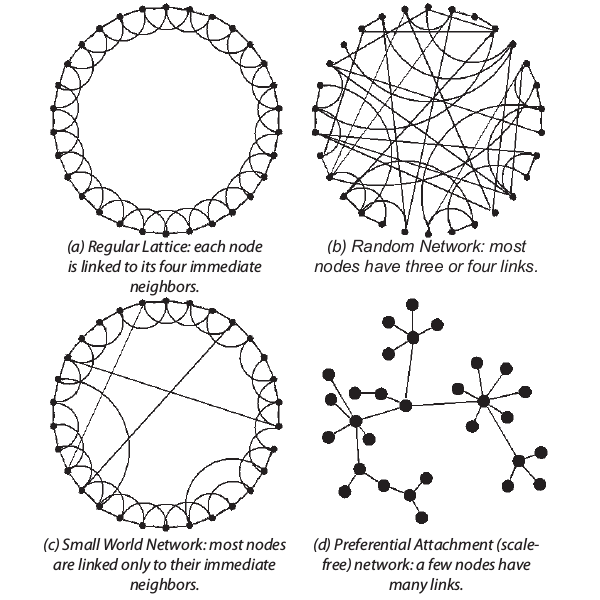
\includegraphics[scale=0.9]{images/Hamill_Gilbert11.png}
\caption{I quattro modelli di rete descritti in \cite{gilbert}}
\end{figure}
Gli autori indicano la costruzione \textit{scale-free} come la migliore tra le quattro, in quanto presenta tutte le caratteristiche elencate in precedenza, con l'eccezione dell'\textit{assortatività}, non particolarmente riflessa nel modello. Passano quindi all'esposizione della loro proposta, un modello ad agenti basato sul concetto di \textit{social circles} \cite{gilbert}: ogni agente può stabilire un ``link" con un altro agente solo se quest'ultimo può fare altrettanto. Quest'idea di \textit{reciprocità} si adatta bene alla modellazione di alcune piattaforme (es. Facebook), mentre si adatta meno su altre: un esempio è Twitter, dove per stabilire un collegamento, il fatto che due utenti si conoscano direttamente è poco rilevante. \\ \\
L'idea che una rete sociale sia assimilabile a una rete ad invarianza di scala (ovvero i cui nodi seguono una \textit{power law}, vedi \ref{subsec:graph}) è largamente supportata in letteratura: testi importanti e fondamentali come \cite{barabasi} e \cite{newman} asseriscono che i social network, così come il World Wide Web stesso, siano organizzati in modo tale che pochi nodi abbiano molti collegamenti e siano collegati tra di loro, mentre molti nodi abbiano pochi collegamenti e siano collegati ad alcuni di questi ``hub". Entrambi i testi, così come \cite{gilbert}, ricordano però l'assunzione \textit{small-world}, che, specialmente per i social network, debba essere verificata. 
\\
\\
Un altro lavoro che abbiamo recuperato è quello di Liben-Nowell \& Kleinberg \cite{link}. Il problema da loro affrontato è quello della previsione di collegamenti (\textit{link prediction}) nei social network, ovvero prevedere, dato lo stato del sistema in un dato istante di tempo, la formazione di nuovi collegamenti negli istanti immediatamente successivi. In una simulazione \textit{dinamica} di una rete è fondamentale stabilire un metodo per cui nuovi collegamenti vengono stabiliti tra i nodi. Un aspetto cruciale in questo caso è il criterio con cui viene valutata la \textit{similarità} tra i nodi del grafo, ovvero come viene assegnato uno \textit{score} a una coppia di nodi (arco) in modo che ne misuri la \textit{``distanza"} rispetto ad una particolare proprietà o caratteristica. Nodi simili ma non ancora collegati avranno infatti un'alta probabilità di stabilire un collegamento negli istanti di tempo più prossimi. \\
Nell'articolo viene fatta una rassegna dei metodi principali; l'obiettivo di questi metodi è costruire la matrice di similarità :
\begin{description}
\item[Neighborhood-based methods] Di questa categoria fanno parte tutti quei metodi che si basano sul \textit{vicinato} (\textit{neighborhood}) dei nodi di cui si vuole calcolare la similarità. La misura di distanza può essere il numero di nodi adiacenti in comune, oppure la probabilità che i due nodi in esame abbiano un vicino in comune, per esempio usando la \textit{distanza di Jaccard}. In alternativa, questa probabilità può essere calcolata in modo proporzionale alla dimensione dei vicinati dei due nodi candidati, per esempio moltiplicandone la cardinalità.
\item[Paths-based methods] Anche la distanza intesa come lunghezza di un cammino tra due nodi può essere intesa come misura di similarità; per esempio, in \cite{katz} viene descritta una metrica che prende in considerazione la lunghezza tutti i cammini esistenti tra due nodi per quantificarne la similarità. Anche alcuni celebri algoritmi, come il \textit{PageRank} di Google \cite{google}, fanno parte di questa categoria.
\end{description}
Altre tecniche possono essere usate in congiunzione con i metodi sopra elencati, per semplificarne la computazione oppure per irrobustirne la previsione. Procedure di \textit{clustering} o \textit{matrix factorization} possono aiutare ad eliminare i collegamenti meno significativi prima dell'effettivo calcolo delle metriche. \\
\\
Essendo però il nostro obiettivo la simulazione di una \textit{social} network, non si può ignorare la (forte) componente sociale del sistema considerato. Ogni nodo rappresenta un utente, e dunque ne eredita le caratteristiche personali come interessi e carattere. La letteratura specializzata in \textit{social sciences} ha da tempo definito il concetto di \textit{omofilia} (\textit{homophily}) \cite{homo} \cite{newman}, inteso come la tendenza di ogni individuo a stringere legami con altri individui dalle caratteristiche simili. Nel computo della misura di similarità (o dissimilarità) bisognerebbe quindi tenere conto di tali caratteristiche e trovare quindi il modo di rappresentarle nel sistema. In \cite{group}, per esempio, gli autori hanno tentato di tradurre in linguaggio matematico l'idea di omofilia, in particolare per quanto riguarda l'aggregazione di individui in base al gruppo di appartenenza. Dopo aver effettuato un'etichettatura degli individui in base a questi raggruppamenti, hanno definito un indice  $H_i$ per l'omofilia:
\begin{equation}
H_i = \dfrac{s_i}{s_i + d_i}
\end{equation}
dove $s_i$ indica il numero medio di \textit{amicizie} (\textit{friendships}) che un individuo facente parte del gruppo $i$ ha con i membri dello stesso gruppo, mentre $d_i$ indica il numero medio di \textit{amicizie} che un membro del gruppo $i$ ha con gli individui appartenenti ad altri gruppi. Questa misura, se confrontata con la frequenza relativa $w_i$ degli individui apparteneti al gruppo $i$, fornisce un indicazione del comportamento degli agenti all'interno del sistema, ovvero se tendono a stabilire conllegamenti fra individui dello stesso gruppo (\textit{inbreeding homophily}) oppure con individui apparteneti ad altri gruppi (\textit{heterophily}).\\
Occorre notare come, nell'ambito dei social network, il termine \textit{omofilia} e il termine \textit{assortatività} siano spesso indicati come sinonimi. \cite{assor} e \cite{mixing} per esempio, forniscono rispettivamente una misura di assortatività per attributo e per grado (vedi \ref{subsec:graph}), ovvero un indice di quanto i vertici di una rete siano legati a nodi con simili valori per l'attributo considerato oppure con simili gradi di archi entranti o uscenti.
\\
\\
Esistono modelli agent-based oltre a quello esposto in \cite{gilbert}, per esempio quelli descritti in \cite{red} e \cite{det}; entrambi usano una rete \textit{scale-free} come ambiente per gli agenti (il primo orientata, la seconda non orientata), ed entrambi regolano gli eventi che accadono nel sistema e le azioni degli agenti secondo degli spazi di probabilità, che si aggiornano dinamicamente. Queste probabilità sono in funzione dell'\textit{in-degree} di ogni nodo e della \textit{similarità} tra ogni coppia di nodi. In particolare, \cite{red} contempla anche l'aggiunta e la delezione di nodi durante la simulazione, operazioni anch'esse regolate da una specifica distribuzione di probabilità. \\
\\
Un'ultima risorsa da noi sfruttata è stata la relazione stilata da Marco Comi e Marco Gravina che, come noi e prima di noi, si sono cimentati nella simulazione del social network Twitter. Abbiamo preso spunto dalle loro soluzioni e dalle criticità del loro modello per sviluppare la nostra proposta.
\section{Riferimenti matematici}
Di seguito descriviamo brevemente alcuni concetti matematici fondamentali per la comprensione delle sezioni successive.
\label{sec:mat}
\subsection{Cosine similarity}
\label{subsec:cos}
Il \textit{coseno di similitudine} (\textit{cosine similarity}) \cite{ir} è una misura di similarità tra due vettori $v_1$ e $v_2$, definita in questo modo:
\begin{equation}
sim(v_1,v_2) = \dfrac{v_1v_2}{|v_1||v_2|}
\end{equation}
dove il numeratore rappresenta il \textit{prodotto scalare} tra i due vettori, mentra il denominatore rappresenta il prodotto dei moduli. I valori possibili ricandono nell'intervallo $[-1,1]$, dove $1$ si ottiene in caso di vettori identici, mentre $-1$ in caso di completa dissimilarità (vettori opposti). 
\subsection{Teoria dei grafi}
\label{subsec:graph}
Un \textit{grafo orientato} $G$ \cite{cormen} è una coppia $(V,E)$, dove $V$ (insieme dei \textit{vertici}) è un insieme finito ed $E$ è una relazione binaria in $V$.\\
Se $(u,v)$ è un arco \cite{cormen} di un grafo $G = (V,E)$ diciamo che il vertice $v$ è \textit{adiacente} al vertice $u$.\\
Dato un grafo $G$ orientato \cite{cormen}, il \textit{grado uscente} (\textit{out-degree}) di un vertice è il numero di archi che escono dal vertice; il \textit{grado entrante} (\textit{in-degree}) è il numero i archi che entrano nel vertice. \\
Un cammino (\textit{path}) \cite{barabasi} da un vertice $v_0$ a un vertice $v_n$ è una lista ordinata di archi $P = \{(v_0,v_1),(v_1,v_2),...,(v_{n-1},v_n)\}$, e $n$ corrisponde alla lunghezza di questo cammino. \\
\\
Un grafo orientato $G$ si dice \textit{completo} \cite{barabasi} quando ogni coppia di vertici è collegata da una coppia simmetrica di archi. La definizione è analoga al caso in cui il grafo sia non orientato, con la differenza che, in quest'ultimo, ogni coppia di archi opposti situata tra due nodi è sostituita da un solo arco non orientato. Il numero di archi \cite{barabasi} in un grafo \textit{non orientato completo} è pari a $\tfrac{N(N-1)}{2}$, dove $N$ è il numero di vertici del grafo. Se si escludono i \textit{cappi} (\textit{self-loops}), allora un grafo \textit{orientato completo} è composto da $N(N-1)$ archi. \\
\\
Si dice \textit{densità della rete} il rapporto tra il numero di archi esistenti e il numero di archi possibili (es. un grafo con densità al 50\% sarà composto da un numero di archi che è pari alla metà del totale di archi possibili).
\subsubsection{Coefficiente di clustering}
Il \textit{coefficiente di clustering} (\textit{clustering coefficient}) \cite{barabasi}, in un grafo \textit{non orientato}, cerca di esprimere il grado con cui i vicini di un dato nodo sono collegati tra di loro. Questo fornisce un'idea della compattezza del gruppo in cui è inserito quello specifico nodo. E' possibile inoltre avere una misura globale della tendenza dei nodi a ``raggrupparsi" calcolando il \textit{coefficiente di clustering medio} (\textit{average clustering coefficient}). Nei grafi orientati  \cite{newman} è disponibile una misura analoga, chiamata \textit{coefficiente di clustering globale} (\textit{global clustering coefficient}, a volte anche chiamata \textit{ratio of transitive triplets} \cite{barabasi}); la sua definizione è la seguente:
\begin{equation}
C_\Delta=\dfrac{3\times NumeroDiTriangoli}{NumberoDelleTripleConnesse}
\end{equation}
dove per \textit{triangolo} si intende un insieme di $3$ vertici, ognuno dei quali connesso agli altri due da archi, mentre per \textit{tripla connessa} si intende tre vertici $uvw$ connessi dagli archi $(u,v)$ e $(v,w)$. I valori possibili ricadono nell'intervallo $[0,1]$.
\subsubsection{Assortatività}
Una rete si dice \textit{assortativa} (\textit{assortative}) \cite{newman} se 
una frazione significativa dei suoi archi collegano vertici simili tra di loro. La similitudine può essere calcolata rispetto a un particolare attributo dei nodi, o, in alternativa, rispetto al \textit{grado} dei vertici. In quest'ultimo caso, in un grafo diretto \cite{assor} la \textit{in-assortativity} e la \textit{out-assortativity} misurano rispettivamente la tendenza dei nodi a legarsi con altri nodi che hanno \textit{in-degree} o \textit{out-degree} identico al loro. Sia $r()$ la funzione che calcola la assortatività, e siano indicati i due tipi di assortatività appena descritti come $r(in,in)$ e $r(out,out)$, è possibile estendere la portata della definizione definendo anche $r(in,out)$ e $r(out,in)$. Supponendo di voler calcolare $r(in,out)$, si ricorre alla seguente formula \cite{mixing}
\begin{equation}
r=\dfrac{\sum_{jk}jk(e_{jk}-q^{in}_jq^{out}_k)}{\sigma_{in}\sigma_{out}}
\end{equation}
dove $e_{jk}$ è la probabilità che un arco qualsiasi conduca da un nodo con \textit{in-degree} $j$ a un nodo con \textit{out-degree} $k$, $\sigma_{in}$ è la deviazione standard della distribuzione $q^{in}$ e $\sigma_{out}$ è la deviazione standard della distribuzione $q^{out}$. La distribuzione di probabilità $q^{out}_k$ (e analogamente $q^{in}_j$) è calcolata come segue:
\begin{equation}
q^{out}_k=\dfrac{(k+1)p^{out}_{k+1}}{\sum_kkp^{out}_k}
\end{equation}
dove $p^{out}_k$ è la probabilità che un nodo abbia \textit{out-degree} $k$. Al denominatore si trova l'out-degree medio della rete.
L'assortatività per attributo è analoga, e si calcola in questo modo:
\begin{equation}
r=\dfrac{\sum_{xy}xy(e_{xy}-a_xb_y)}{\sigma_a\sigma_b}
\end{equation}
dove $e_{xy}$ è la probabilità che un arco qualsiasi conduca da un nodo con valore dell'attributo $x$ a un nodo con valore $y$, mentre $a$ e $b$ sono rispettivamente le frequenze degli archi che escono ed entrano in un nodo con valori $x$ e $y$. In entrambi i casi il valore di $r$ ricade nell'intervallo $[-1,1]$, con $1$ a indicare la perfetta assortatività e $-1$ la perfetta disassortatività.   
\subsubsection{Rete a invarianza di scala}
Una rete viene indicata come \textit{rete a invarianza di scala} (\textit{scale free network}) se la distribuzione dei gradi dei nodi (probabilità $p(k_i)$ che un nodo scelto in modo random abbia grado $k_i$) segue una \textit{power law} \cite{scalefree}.\\
Una \textit{power law} \cite{barabasi} è una funzione $y=f(x)$ in cui il valore $y$ della funzione è proporzionale ad una potenza del valore in ingresso $x$:
\begin{equation}
\label{eq:power}
p_x \sim x^{-\gamma}
\end{equation}
L'equazione \ref{eq:power} è chiamata \textit{power law distribution} e l'esopente $-\gamma$ è detto \textit{degree exponent}. La rappresentazione con il logaritmo dell'equazione \ref{eq:power} diventa
\begin{equation}
\label{eq:power2}
\log p_x \sim -\gamma \log p
\end{equation}
Se vale l'equazione \ref{eq:power2}, allora ci si aspetta che $\log p_x$ dipenda linearmente da $\log x$, con inclinazione della retta pari a $\gamma$, come indicato nella figura \ref{fig:power}. Assumendo che il grado di un nodo sia una quantità discreta, si può adottare il formalismo per il discreto; in questo modo, l'equazione \ref{eq:power} diventa
\begin{equation}
p_x \sim Cx^{-\gamma}
\end{equation} 
dove $C$ è una costante.
\begin{figure}[h]
\centering
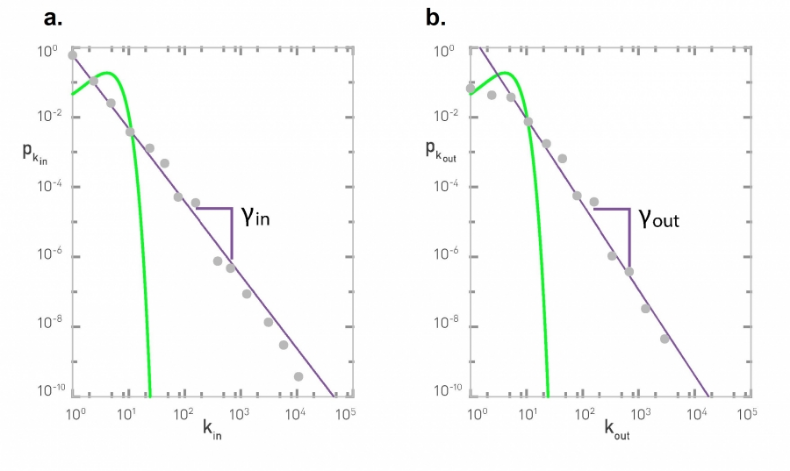
\includegraphics[scale=0.6]{images/powerlaw.png}
\caption{Distribuzione del WWW misurata nel 1999 \cite{barabasi}. La figura a. rappresenta la distribuzione dei nodi rispetto all'\textit{in-degree}, mentre b. rispetto all'\textit{out-degree}. Entrambe usano una scala logaritmica.}
\label{fig:power}
\end{figure}
\section{Descrizione modello} 
\label{sec:mod}
Abbiamo cercato di creare un modello che rispecchi il pi\`u possibile il modo in cui Twitter viene utilizzato nella realt\`a da utenti umani. Ovviamente alcune restrizioni e semplificazioni sono state effettuate per creare un modello realizzabile sia dal punto di vista concettuale che computazionale. Tuttavia ABSoNeS risulta essere una buona base per la simulazione di social network, come verrà descritto più avanti. Alcune delle semplificazioni pi\`u rilevanti possono comunque essere introdotte in futuro senza la necessit\`a di stravolgere il modello attuale, ma arricchendolo con relativa semplicit\`a.
\\ \\
ABSoNeS è composto da un \textit{grafo} i cui nodi rappresentano gli \textit{utenti} (quindi gli \textit{agenti}) di una rete sociale ispirata a Twitter. Ogni nodo può produrre oggetti (tweet e retweet) e stabilire o interrompere collegamenti secondo delle \textit{probabilità} (statiche o dinamiche); l'agire o meno di questi utenti è determinato secondo un campionamento di tipo Monte Carlo su queste probabilità. Ogni nodo ha degli attributi che lo rendono unico, dunque ognuno di questi agenti sviluppa un comportamento che lo identifica, ed è parzialmente influenzato dalle azioni degli agenti con cui è in contatto. 
\\ \\
Di seguito elenchiamo gli elementi chiave comuni a tutti gli utenti. Tali aspetti servono a descrivere le caratteristiche personali degli utenti, in particolare il loro periodo di attivit\`a durante il giorno e i loro interessi personali.
Questi elementi sono al momento immutabili dopo la creazione dell'utente, per quanto questa possa sembrare una forte restrizione, non \`e sbagliato assumere che mediamente gli interessi e gli impegni lavorativi di una persona non cambino nell'arco di qualche mese, che \`e l'obiettivo della simulazione.
\begin{description}
  \item[Fasi Temporali (FT)] Dividiamo la giornata in 12 fasi che 
    rappresentano 2 ore l'una in cui ogni utente ha un personale
    valore di \textit{activity} che rappresenta il suo utilizzo di Twitter.
    Tali fasi sono cos\`i suddivise:
    \begin{itemize}
      \item 4 fasi con \textit{activity} pari a 0 corrispondente a 8
      ore di sonno, ovvero la quantit\`a consigliata (e quasi mai 
      rispettata);
      \item 4 fasi con \textit{activity} bassa, corrispondente a 8 ore di 
      lavoro;
      \item 4 fasi con \textit{activity} elevata che rappresenta 8 ore di 
      tempo libero in cui l'utente ha una attivit\`a maggiore su 
      Twitter.
    \end{itemize} 

  \item[Topic] ovvero i possibili argomenti di interesse esistenti 
    nel modello perci\`o abbiamo una lista \textit{topic} 
    $ = (t_1, \dots , t_n) $ definiti a priori e immutabili. 
    Non vengono mai utilizzati direttamente, ma vengono utilizzati 
    come indici di riferimento dunque non \`e necessario 
    implementarli realmente.
\end{description}

\subsection{Utenti}
\label{subsec:users}
Gli utenti sono i nodi della rete. Di seguito mostriamo come gli utenti sono rappresentati nel modello, in particolare ogni utente \`e caratterizzato da:

\begin{description}
  \item[Personal Interest (PI)] \`e un vettore di probabilità $PI$ 
    $=(p_1, \dots, p_n)$ dove $p_i \in (0, 1)$.
    indica la probabilit\`a di interesse del nodo rispetto al 
    \textit{topic} $i$ generata casualmente. Da notare che $\sum_{i=1}^n p_i = 1$.
  \item[Timezone (TZ)] ovvero una lista $TZ$ $=(tz_1, \dots, tz_{12}) $
  dove i $tz_i$ sono generati in accordo con le \textbf{FT} 
  come segue:
  \begin{itemize}
    \item Viene scelto un indice $1\leq i \leq 12$ casualmente
    \item Si impostano le ore di sonno $tz_j = 0$ per $j = i, \dots , i+3$
    \item Si impostano le ore di lavoro $tz_j$ = bassa \textit{activity} per 
      $j = i+4, \dots , i+7$
    \item Si impostano le ore di tempo libero $tz_j$ = alta \textit{activity}
      per $j = i+8, \dots , i+11$
  \end{itemize}
  Tutte le precedenti operazioni di indici sono da considerarsi 
  $mod \quad 12$. Il motivo di questa scelta \`e quello di simulare
  sia diversi orari per le persone, come ad esempio lavori notturni, sia diversi fusi orari cercando di distribuire uniformemente gli orari personali. Nel codice, i valori per alta e bassa activity sono probabilità, e vengono generate usando una distribuzione triangolare con i seguenti parametri:
  \begin{itemize}
  \item Bassa activity: $a = 0$, $m = 0.25$, $b = 0.6$  
  \item Alta activity: $a = 0.4$, $m = 0.75$, $b = 1$ 
  \end{itemize}
\end{description}
Ogni utente \`e inoltre caratterizzato dalle seguenti propriet\`a:

\begin{description}
  \item[Followers] per ogni utente U definiamo come \textit{followers}(U) 
  l'insieme dei followers di U. Il loro numero è pari all'\textit{in-degree} del nodo U.
  \item[Following] similmente al precedente \textit{following}(U) indica
  l'insieme degli utenti seguiti da U. Il loro numero è pari all'\textit{out-degree} del nodo U.
  \item[Direct Tag (dtag)] \textit{dtag}(U, T) \`e l'insieme dei tweets che
  contengo un tag all'utente U generati al tempo T. 
  Una descrizione pi\`u dettagliata \`e disponibile nella sezione
  riguardante i tweet [\ref{subsec:social}].
  \item[Field Of View (FOV)] \textit{FOV}(U, T) rappresenta l'insieme dei
  delle notizie visualizzate dall'utente U al tempo T, con 
  \textit{FOV} $\subseteq$ \textit{tweet}(\textit{following}(U), $T_i$) $\cup$ 
  \textit{retweet}(\textit{following}(U), $T_j$) $\cup$ \textit{dtag}(U, $T_l$) 
  per $T_{i,j,l} \in \overline{T}$ lista di
  tempi non maggiori al tempo attuale T.
  Questo insieme \`e definito sia per una questione
  computazionale, ma anche per un motivo reale in quanto \`e 
  difficile che un utente nell'arco della giornata riesca a vedere
  tutti i tweets e i retweets degli utenti che segue e i tweet che
  in cui risulta direttamente \textit{taggato}. Questa affermazione
  diventa sempre pi\`u ragionevole al crescere della popolarit\`a 
  di un utente.
\end{description}

Ovviamente un grafo senza archi non rappresenterebbe nulla, cos\`i come un simulatore di social network senza interazione tra gli utenti; perci\`o di seguito viene mostrato come sono definiti gli archi e che caratteristiche hanno e pi\`u in seguito le possibili interazioni tra gli utenti.

\begin{description}
  \item[Edges] un arco tra due utenti $U_1$ e $U_2$, scritto come
  $(U_1 ,U_2)$ rappresenta la relazione di following tra il primo 
  ed il secondo. Di conseguenza, ovviamente, 
  risulta che $U_1 \in $  \textit{followers}($U_2$) e simmetricamente
   $U_2 \in $  \textit{following}($U_1$)
   \item[Attachment] ad un arco $e_j \in U\times U$ \`e associato un 
   valore \textit{attach}($U_1, U_2$) $ \in [0,1]$ che rappresenta l' 
   \textit{attaccamento} di $U_1$ a $U_2$, pi\`u questo valore si 
   avvicina a 0 pi\`u la probabilit\`a che $U_1$ smetta di seguire
   $U_2$ aumenta e viceversa. Quando l'arco viene creato il valore
   di \textit{attach} \`e relativamente alto (si usa una distribuzione triangolare con parametri $a = 0.5$, $m = 0.8$, $b = 1$) in quanto ci si 
   aspetta che un utente non smetta di seguire un altro utente
   poco dopo aver iniziato a seguirlo.
\end{description}

\subsection{Attivit\`a di base}
\label{subsec:prob}

Elenchiamo qui le azioni che ogni utente può effettuare. Queste azioni vengono decise sulla base di estrazioni Monte Carlo: estratto un numero casuale, se ricade entro un certo intervallo di probabilità l'azione viene compiuta.

\begin{description}
  \item[Tweet] Posto $x = \dfrac{|followers(U)|}{|Users|}$ ogni utente U ad ogni tempo T ha la possibilit\`a
  di creare un tweet secondo la seguente probabilit\`a:
    \begin{equation}
    \label{eq:ptwt}
      P_{tweet} = \alpha TZ(T) (-\dfrac{\log{(x+4)}}{  \log{(x+2)}} +2)
    \end{equation}
  Questo perch\`e ci si aspetta che un utente popolare sia pi\`u 
  attivo di uno sconosciuto, per mantenere il suo livello di 
  popolarit\`a. Questa \`e una rappresentazione della realt\`a che contiene una restrizione, in quanto esistono esempi di persone poco conosciute che producono molti tweets, e di persone molto famose che non usano mai i social, soprattutto i pi\`u anziani. Tuttavia \`e ragionevole pensare che la precedente assunzione sia mediamente vera. La funzione \ref{eq:ptwt} cerca di tradurre questo concetto in uno spazio di probabilità: più il rapporto $x$ tende a 1, più la funzione cresce, ma in maniera logaritmica, in modo che quando $x = 1$ si ha che $P_{tweet} \approx 0.5 $; questo è per evitare la  iperattività degli agenti, e prevenire così il completamento della rete. $\alpha$ è un fattore di normalizzazione, ottenuta sommando $P_{tweet}$ a $  P_{\neg tweet}$:
  \begin{equation}
    \label{eq:ptwt}
      P_{\neg tweet} = \alpha (1 - TZ(T)) (1 - (-\dfrac{\log{(x+4)}}{  \log{(x+2)}} +2))
    \end{equation}
  
  \item[Retweet] La probabilità $P_{retweet}$ è calcolata col medesimo meccanismo di $P_{tweet}$
    Nel modello assumiamo per semplicit\`a che un utente possa produrre al massimo un retweet ad istante di tempo. Una possibile versione futura potrebbe rilassare questo vincolo rendendo ancora pi\`u simile alla realt\`a il modello.
    
  \item[Tag] Ogni tweet ha una possibilit\`a di contenere un tag 
  diretto ad un altro utente V. Tuttavia per questa caratteristica non \`e possibile fare delle assunzioni che possano essere verosimili, in quanto twetter permette ad un qualunque utente di taggare un qualunque altro utente. Perci\`o abbiamo deciso di implementare un sistema randomico dove ogni utente ha il 20 \% di probabilit\`a di taggare un altro qualsiasi utente. 
  Grazie proprio a questa particolare caratteristica \`e possibile che accadano, sia nella realt\`a che nel modello casi particolari come quello descritto nella fase sperimentale.
\end{description}

\subsection{Attivit\`a sociali}
\label{subsec:social}
\`E importante definire quali sono le attivit\`a sociali che gli utenti possono fare per interagire tra di loro. Queste attività hanno come oggetto di scambio fra gli utenti i seguenti oggetti:

\begin{description}
  \item[Tweet] Il tweet dell'utente U al tempo T \`e definito come
  \textit{tweet}(U,T) = ($j$, \textit{likability}, \textit{dislikability}, \textit{dtag}
  %, U, T
  ) dove:
  \begin{itemize}
    \item $j$ \`e il \textit{topic} su cui il tweet verte
    \item \textit{likability} $\in [0,1]$, indica la probabilit\`a di quanto
    il tweet possa piacere agli utenti a cui interessa il 
    \textit{topic} $j$. 
    \item \textit{dislikability} $\in [0,1]$, rappresenta la probabilit\`a di quanto il tweet 
    possa non piacere a chi non \`e interessato all'argomento
    \item \textit{dtag} indica l'utente V taggato nel tweet. Tale valore 
    pu\`o anche essere nullo.
%    \item U \`e l'utente che ha effettuato il tweet, e T il tempo in
%    cui \`e stato creato.
%    Necessari per l'implementazione.
  \end{itemize}
  
  \item[Retweet] Il retweet effettuato dall'utente U al tempo T
  del tweet di V al tempo $\overline{T}$, definito come:
  \textit{retweet}(U, T) = \textit{tweet}(V, $\overline{T}$)
  
  \item[Dtag] Il tag diretto di un utente U ad un altro utente V al 
  tempo T \`e definito come \textit{dtag}(U, V, T) = tweet(U, T) e 
  rappresenta il caso in cui l' utente U ha ``taggato'' V con un 
  \textit{@U}. Questo permette all'utente V di vedere un tweet 
  di U, anche nel caso in cui non lo seguisse.
\end{description}
In base agli oggetti definiti in precedenza possiamo definire le 
azioni di:

\begin{description}

  \item[Post] Nel momento in cui l'utente U \`e abilitato alla 
  creazione di un tweet viene generato casualmente un 
  \textit{topic} $j$ su cui verter\`a il tweet in modo tale che un topic 
  di interesse per U sia selezionato con maggiore probabilit\`a.
  Una volta scelto il topic $j$:
  \begin{itemize}
    \item se $j$ \`e di interesse per U (U.$PI$($j$) $\geq 0.5$)
     allora il \textit{tweet} risultante
    avr\`a una \textit{likability} elevata mentre la \textit{dislikability} sar\`a casuale.
    \item viceversa il \textit{tweet} generato avr\`a una \textit{dislikability} alta ed
    una \textit{likability} casuale.
  \end{itemize}
  Una volta definito il tweet viene generata la probabilit\`a di 
  avere un \textit{dtag} ad un altro utente V. Se tale tag viene generato allora il \textit{tweet} avr\`a
  un tag all'utente V, altrimenti il post non avr\`a alcun \textit{dtag}.
  
  \item[Repost] Per ogni utente U viene scelta casualmente una lista 
  di $k$ \textit{tweet} $\overline{w} \in$ \textit{FOV}(U)$^k$, successivamente
  per ogni $\overline{w}_i \in \overline{w}$ viene valutata la 
  possibilit\`a di retweet di $\overline{w}_i$ secondo l' equazione
  \ref{eq:ptwt}, in caso favorevole viene prodotto \textit{retweet}(U, T) 
  che sar\`a una lista di retweet effettuati da U al tempo T.
  \item[Unfollow] Ad ogni istante T di tempo, ogni nodo ha lo $0.5\%$ di possibilità di intraprendere un'attività di valutazione dell'attachment che intercorre tra lui e gli utenti da lui seguiti. La valutazione avviene secondo il seguente algoritmo:
  \begin{enumerate}
  \item Genera il $FOV$ per l'utente $U_1$.
  \item Scorri tutti gli elementi (tweet o retweet) presenti nel $FOV$
  \item Aggiorna l'attachment con il nodo $U_2$ che ha effettuato il tweet o il retweet:
  \begin{enumerate}
  \item Se il topic dell'elemento è di interesse dell'utente (topic maggiore della media dei valori del $PI$) allora $attach(U_1,U_2)_{new} = \dfrac{attach(U_1,U_2)_{old}+ likability}{2}$
  \item Se il topic dell'elemento no è di interesse dell'utente (topic minore della media dei valori del $PI$) allora $attach(U_1,U_2)_{new} = \dfrac{attach(U_1,U_2)_{old}+ dislikability}{2}$
  \end{enumerate}
  \item Elimina il collegamento con il nodo con il minore attachment
  \end{enumerate}
  L'idea originale era quella di valutare l'attachment di tutti gli archi ad ogni istante T: questo è chiaramente un compito oneroso che, specialmente in reti con elevata densità, aumenta enormemente i tempi di esecuzione. Inoltre, non rispecchia appieno il processo di unfollow reale, poichè nessun utente umano valuta regolarmente l'interesse verso ogni suo collegamento. Per cui abbiamo abbandonato questa soluzione in favore dell'algoritmo appena descritto.
  \item[Follow] Esistono due tipi di possibili modalit\`a di 
  following:
    \begin{description}
      \item[By Retweet (BR)] 
      Nel caso in cui nel FOV compaia un retweet di un utente non 
      seguito, si pu\`o decidere di seguirlo attraverso la seguente 
      valutazione: si considerano gli ultimi $n$ \textit{tweet} e \textit{retweet} (a partire dall'istante $T = -20$)
      dell'utente target e da questi si inferiscono i suoi interessi.
      Dal momento che per un utente non \`e possibile conoscere il vettore di probabilit\`a privato di un altro utente, esso viene inferito dal potenziale follower che ha intenzione di seguirne un altro valutando i topic dei suoi precedenti tweet, e la loro compatibilit\`a viene valutata utilizzando la cosine similarity che, siccome ha a che fare con vettori di probabilità, assumerà valori nell'intervallo [0,1]. L'operazione di follow andrà a buon fine se il valore estratto è \textit{minore} del valore di distanza calcolato in questo modo.
    Questa scelta \`e giustificata dal fatto che nella realt\`a non \`e possibile conoscere gli interessi di un'altra persona se non inferendola da ci\`o che condivide, oppure attraverso un fattore di intuito umano, che chiaramente gli utenti simulati non hanno.
      \item[Outside Factor (OF)] avviene quando un utente U comincia
      a seguire un nodo V per fattori esterni al Social Network, 
      quali ad esempio nuova amicizia nella vita reale, nuovo
      follow su altri mezzi di comunicazioni online, ecc. Questa operazione è speculare all'unfollow: ad ogni istante di tempo $T$ ogni nodo ha lo $0.5\%$ di possibilità di iniziare a seguirne un altro, estratto a caso dall'insieme di utenti. 
	  
    \end{description}
\end{description}



\subsection{Step Simulazione}
\label{subsec:step}

Usando tutte le azioni definite in precedenza possiamo ora descrivere gli 
step che avvengono nella simulazione ad ogni istante di tempo T.

\begin{description}
  \item[Tweet Step (TS)] Per ogni utente U viene generato una 
  probabilit\`a casuale $P_t(U,T)$ che rappresenta la sua 
  inclinazione di produrre un \textit{tweet} al tempo T. Se $P_t(U,T)$
  risulta minore alla probabilit\`a $P_{tweet}$ (eq. \ref{eq:ptwt}) allora
  viene generato il \textit{tweet}(U, T) come descritto in \textbf{Post}.
  
  \item[Retweet Step (RS)] Similmente alla fase precedente,
  per ogni utente U viene generato una 
  probabilit\`a casuale $P_r(U,T)$ che rappresenta la sua 
  inclinazione di produrre un \textit{retweet} al tempo T. Se $P_r(U,T)$
  risulta minore alla probabilit\`a $P_{retweet}$ (eq. \ref{eq:ptwt}) 
  allora viene generato il \textit{retweet}(U, T) come descritto in 
  \textbf{Repost}. In questa fase avvengono anche le eventuali valutazioni del \textbf{Follow by retweet}, con la creazione di nuovi archi.
  
  \item[Evaluation Step (ES)] Questa fase comprende le altre due operazioni descritte, ovvero \textbf{Follow by Outside Factor} e l'\textbf{Unfollow}. 
\end{description}

Le azioni descritte in precedenza devono necessariamente essere 
eseguite sequenzialmente una dopo l'altra, tuttavia i singoli step 
possono essere facilmente parallelizzati, senza problemi di 
concorrenza, in quanto il post di un tweet \`e indipendente per ogni
utente; lo stesso vale per il retweet e infine l'aggiornamento dell'
\textit{attach} \`e  dipendente dai tweet e i retweet effettuati 
\textbf{TS} e \textbf{RS}, ma i singoli aggiornamenti sono 
indipendenti tra gli utenti. Per questo motivo \`e 
possibile parallelizzare il modello in modo che 
le azioni contenute in ogni step di simulazione 
vengano effettuate contemporaneamente, ma comunque rispettando l'ordine descritto.
Questa modello di parallelizzazione non \`e tuttavia implementato per questa versione in quanto sarebbe necessario implementare tecniche di sincronizzazione tra le strutture dati che contengono gli elementi della simulazione.
\section{Interpretazione multi-agente}
\label{sec:mas}
Prima di descrivere gli agenti \`e necessario caratterizzare l'ambiente in cui essi operano.
Nel modello descritto in precedenza l'ambiente \`e formalizzato come un grafo diretto in cui i nodi sono gli agenti e gli archi sono le connessioni tra di essi e il peso \`e la forza del loro legame.
Questo tipo di ambiente \`e tendenzialmente inaccessibile in quanto gli agenti hanno visione solo dell'ambiente che li circonda; per\`o ci sono delle eccezioni. \`E possibile che un utente abbia accesso ad una parte di ambiente a lui distante nel caso in cui venga taggato da una persona con cui non ha nessun legame, questo \`e il principio su cui la fase 2 degli esperimenti si basa. Esiste inoltre il caso degenere in cui un particolare agente \`e connesso a tutti i nodi e quindi ha potenzialmente accesso a tutto l'ambiente, tuttavia in questo caso la sua visione \`e limitata dal suo FOV. Per via del fatto che gli utenti basano le proprie azioni su un modello probabilistico l'ambiente risulta non deterministico, in quanto non \`e possibile prevedere con certezza il suo stato successivo. Possiamo definire l'ambiente come episodico in quanto ogni utente prende decisioni in base allo stato in cui attualmente si trova la simulazione senza considerare le i possibili effetti nel futuro. Risulta complicato definire se gli angeti si trovino in contesto statico o dinamico o dinamico e discreto o continuo, in quanto non si applica completamente a nessuna delle due possibili definizioni. L'ambiente risuta statico perch\`e non ci sono processi che sono al di fuori del controllo degli utenti (tale concetto non \`e pi\`u veritiero nel caso in cui venga implementata in una versione futura la crescita del grafo iniziale), tuttavia gli agenti producono degli artefatti che modificano in qualche modo l'ambiente e le future interazioni delle sue componenti.
Inoltre possiamo definire la simulazione come discreta, in quanto esiste un numero predefinito di azioni che gli utenti possono compiere, ma le percezioni che gli utenti hanno dello stesso cambiano ad ogni step. I metodi di interazioni permesse sono descritte pi\`u in dettaglio nel seguito.

Gli agenti all'interno del modello ABSoNeS possono essere visti come agenti un ibrido tra hysteretic e knowledge-based. Le loro azioni nel modello agent-based vengono classificate come:
\begin{description}
    \item[See] Gli agenti, o utenti in questo caso,
    osservano l'ambiente che li circonda; ovvero guardano chi li segue e chi loro seguono. Inoltre vedono gli elementi presenti nell'ambiente quali tweet, retweet e tag diretti. Tuttavia hanno una visione limitata di ci\`o che li circonda. Sono infatti in grado di visionare solo l'ambiente che li circonda che in questo caso corrisponde agli altri utenti ai quali sono connessi e alle loro azioni.
    \item[Action] Le modalit\`a in cui gli agenti compiono le loro azioni sociali sono il motivo per cui possono essere classificati come ibridi.
    Questo \`e dovuto al fatto che gli utenti decidono che tweet produrre in base a loro stati interni: activity e personal interest. Tali caratteristiche influiscono sulle azioni personali che ogni utente compie e solo la parte isteretica dell'agente.
    Quando per\`o un agente si trova nella sua fase evaluation prende decisioni in base ad una conoscenza che inferisce da ci\`o che lo circonda. 
    In particolare la decisione di continuare a seguire o di smettere di seguire qualcuno \`e dovuta da un ragionamento effettuato sui tweet, prodotti da altri agenti, che osserva. E il suo valore di attachment varia a seconda di un ragionamento, per quanto banale, basato di essi.
    La parte pi\`u caratterizzante deriva dal ragionamento che ogni agente effettua quando decide di seguire qualcuno. Infatti guardando le azioni di un altro utente inferisce quali possano essere i suoi interessi e se sono compatibili a propri. In caso positivo pu\`o decire di seguirlo, altrimenti no.
    \item[Do] Le azioni che ogni utente pu\`o effettuare sono largamente descritte nella sezione di modellazione, tuttavia riassumento ogni utente \`e in grado di seguire, smettere di seguire; produrre un tweet o un retweet; taggare direttamente un altro utente.
    \item[Internal] Alcuni stati interni dell'utente sono immutabili, ovvero i personal intereset e le time zone. Tuttavia dopo ogni step di simulazione ogni agente aggiorna i suoi valori di attachment verso gli altri utenti.
\end{description}
Gli agenti nel modello sono da considerarsi autonomi su alcuni dei contesti che li caratterizzano; in particolare ogni agente \`e in grado di decire le proprie azioni in base ai suoi stati interni e alla visione dell'ambiente che lo circonda; ha inoltre controllo su alcuni dei suoi stati interni, anche se questo controllo \`e dovuto ad una risposta all'ambiente e non ad una sua decisione. Tuttavia gli utenti non hanno la capacit\`a di prendere decisioni in base alla loro esperienza regressa, ma in ogni caso questo fattore non \`e particolarmente rilevante in quanto possiamo facilmente osservare che spesso nemmeno gli utenti reali dei social network imparano dalle loro azioni. Basti pensare al presidente Trump, che nonostante abbia usato per anni il suo account tweetter per auto-diffamarsi, presumibilmente senza rendersene conto, continua a fare lo stesso nonostante l'importanza della carica che copre.

Per completezza di descrizione risulta essenziale osservare che gli agenti non hanno un obiettivo, n\`e in comune n\`e personale. Potrebbe sembrare che ogni utente abbia come obiettivo quello di aumentare sempre di pi\`u la sua cerchia di followers anche se in realt\`a, per come \`e definito il modello, gli agenti non hanno nessun interesse verso questo obiettivo e nemmeno sono incetivati ad averlo. Cos\`i come per la maggior parte degli utenti reali, gli agenti sono solo interessati ad espreme le loro opinioni senza un obiettivo particolare. Per lo stesso motivo le azioni che compiono non hanno una utilit\`a nei confronti di s\`e stessi, dell'ambiente e degli altri utenti, semplicemente tweettano per il solo piacere di farlo.

\`E difficile caratterizzare in termini classici l'interazione tra gli utenti, in quanto essi non hanno interazione diretta e non si passano nessuna informazione tra loro. Si potrebbe dire che gli agenti comunicano attraverso degli artefatti condivisi (tweet, ecc) avvicinandosi al modello artifact-mediated indirect interaction; tuttavia, nonostante gli artefatti siano condivisi e ci sono delle chiare regole che ne definiscono l'accesso da parte degli agenti, essi non sono un vero e proprio canale di comunicazione ma risultano essere delle ``tracce'' a cui altri agenti decidono se prestare attenzione o meno. Questo \`e dovuto dal fatto che non sia presente nessun obiettivo, comune o personale a cui tutti fanno riferimento.
\section{Esperimenti}
\label{sec:esp}
In questa sezione esponiamo le prove condotte con il nostro modello. 
Abbiamo organizzato gli esperimenti in due fasi: 
\begin{description}
\item[Fase 1] Nella prima fase testiamo la solidità del nostro approccio andando a verificare che la rete rispetti le caratteristiche tipiche di una rete sociale.
\item[Fase 2] Nella seconda fase osserviamo il cambiamento del sistema all'occorrenza di un particolare evento, in particolare studiamo il ``salto" di popolarità da parte di un utente.
\end{description}
Per quanto riguarda la prima fase, uno dei rischi maggiori è produrre un modello incline al \textit{completamento della rete}, ovvero un modello i cui agenti, alla fine della simulazione, sono tutti collegati fra di loro da due archi (essendo un grafo diretto). In un social network reale questa cosa non si verifica, in quanto gli utenti non hanno interesse ad essere collegati con tutti gli altri. Questo è stato uno dei principali obiettivi durante la costruzione del modello, assieme alla conservazione della proprietà di \textit{invarianza di scala} e alla tendenza degli utenti a stabilire collegamenti secondo l'\textit{omofilia}. 
\\
\\
Nella seconda fase simuliamo lo scenario in cui un utente con pochi collegamenti in entrata, ovvero con pochi \textit{follower}, viene ``notato'' da uno degli ``hub", ovvero un utente con molti follower. Per far ciò, forziamo il retweet da parte dell'utente hub di un tweet creato ad-hoc per l'utente meno importante; dopodichè controlliamo la variazione di popolarità  dell'utente prescelto in termini di follower. Questo per simulare quanto avvenuto nel 2012 tra l'On. Maurizio Gasparri e l'utente Daniele Termite \cite{termite} dopo essere stato ``ripreso" su Twitter dall'Onorevole, l'utente Termite ha visto crescere improvvisamente di popolarità il suo account, con un boom di follower nel giro di brevissimo tempo, per poi assestarsi su un numero di circa 10.000 seguaci. La replica \textit{in-silico} di questo fenomeno utilizzando il nostro modello può essere considerata come indica di affidabilità dello stesso.
\\
\\
Per la realizzazione del modello e la conduzione degli esperimenti la scelta implementativa è ricaduta su \textit{Python} (versione 3) e sulla libreria \textit{networkx} \cite{nx}, un package molto curato e completo per la modellazione di reti. In principio avevamo optato per l'ambiente di simulazione PyCx, che fornisce un'interfaccia per la conduzione di esperimenti e la visualizzazione dei risultati, ma abbiamo riscontrato successivamente una incidenza negativa sulle performances del modello; per cui abbiamo virato su una CLI per l'inserimento dei parametri. La visualizzazione dei grafi è stata effettuata con il software Gephi, mentre i grafici delle metriche con R.
\subsection{Fase 1}
Per valutare la buona riuscita degli esperimenti, considerando quanto prodotto dalla letteratura, abbiamo individuato come parametri principali per valutare l'attendibilità della rete prodotta dal nostro modello le seguenti metriche:
\begin{enumerate}
    \item La \textit{densità} della rete, per monitorare la tendenza del modello al completamento o meno della rete.
    \item I parametri della \textit{power law} che intercorre sul grado dei nodi, per studiarne l'invarianza di scala.
\end{enumerate}
Altre metriche che abbiamo incluso nell'analisi sono:
\begin{enumerate}
    \item Il \textit{coefficiente di clustering}, per valutare la predisposizione alla formazione di gruppi di agenti.
    \item L'\textit{assortatività per attributo}, per valutare l'omofilia rispetto ai topic caratterizzanti gli utenti. Come attributo abbiamo scelto il topic con valore più alto nel $PI$ di ogni nodo.
    \item L'\textit{assortatività per grado r(out,in)}, a supporto del punto 2 della lista precedente, ovvero la valutazione dell'invarianza di scala.
    \item Il \textit{cammino minimo medio} (in caso di reti connesse) per verificare l'ipotesi di \textit{small world}
\end{enumerate}
Abbiamo quindi organizzato una sessione di esperimenti con i seguenti parametri comuni:
\begin{itemize}
\item 1000 utenti
\item 10 topic per utente
\item 1080 iterazioni (equivalenti a 90 giorni)
\end{itemize}
La differenza tra le varie run sta nella diversa istanziazione della rete iniziale; non avendo indicazioni sul valore di densità del grafo reale di Twitter, abbiamo optato per due soluzioni principali:
\begin{itemize}
\item Istanziazione di una rete scale-free, a densità fissa
\item Istanziazione di una rete random, a densità variabile
\end{itemize}
Il package networkx di Python permette l'istanziazione di una rete scale-free con una densità non modificabile pari a circa $0.1\%$: questo è dovuto al particolare modello usato dalla libreria, descritto in \cite{sfnx}, che per rispetto alla power law non permette la scelta del numero di archi iniziale.
A questa abbiamo quindi affincato una serie di prove con una random network come configurazione di partenza, avente valori diversi come densità iniziale: nello specifico, i valori sono $0.1\%$, $0.5\%$, $1.0\%$ e $5.0\%$.
\subsubsection{Risultati}
Le figure \ref{fig:sf1}, \ref{fig:rnd01}, \ref{fig:rnd05}, \ref{fig:rnd1} e \ref{fig:rnd5} mostrano l'andamento dei quattro indici che abbiamo scelto per la valutazione.
\begin{figure}[h]
\begin{tabular}{cc}
  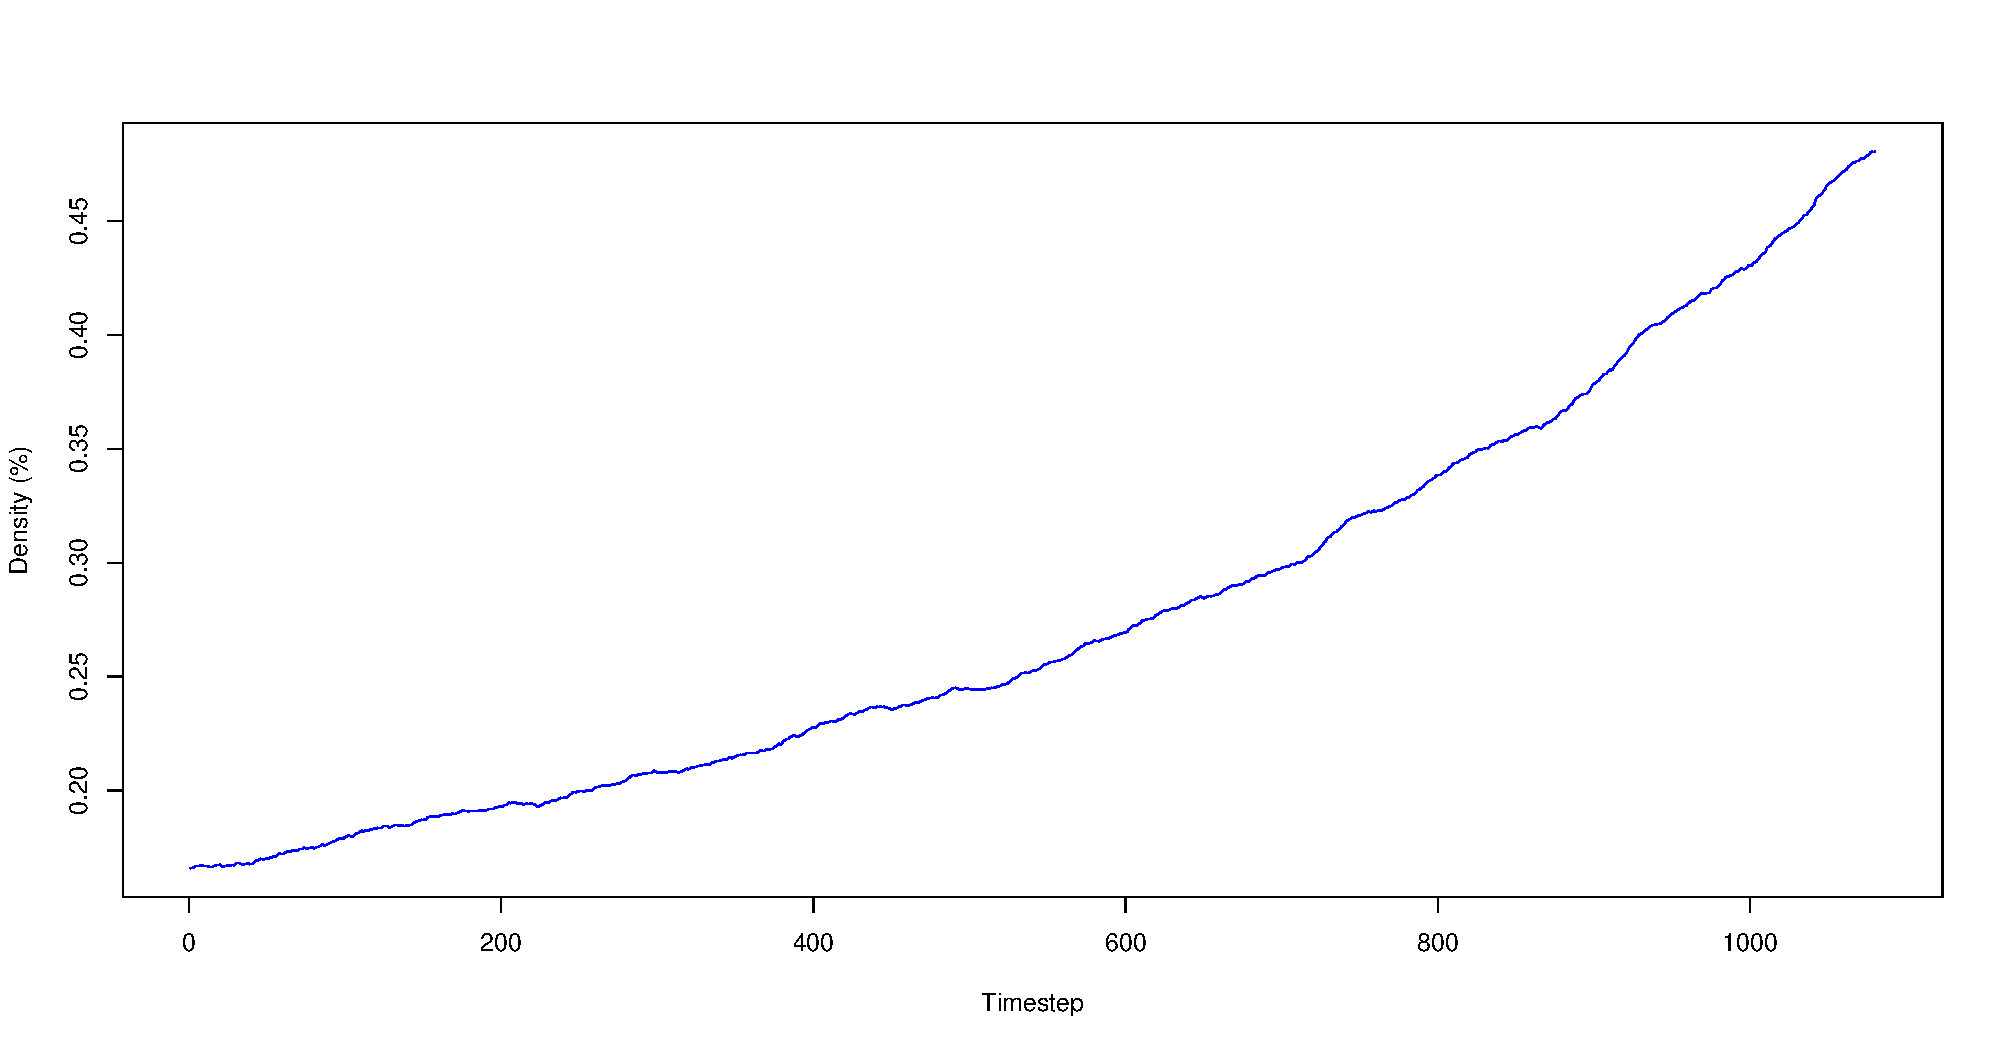
\includegraphics[width=83mm]{images/evolution_1000_sf_1080_0.pdf} &   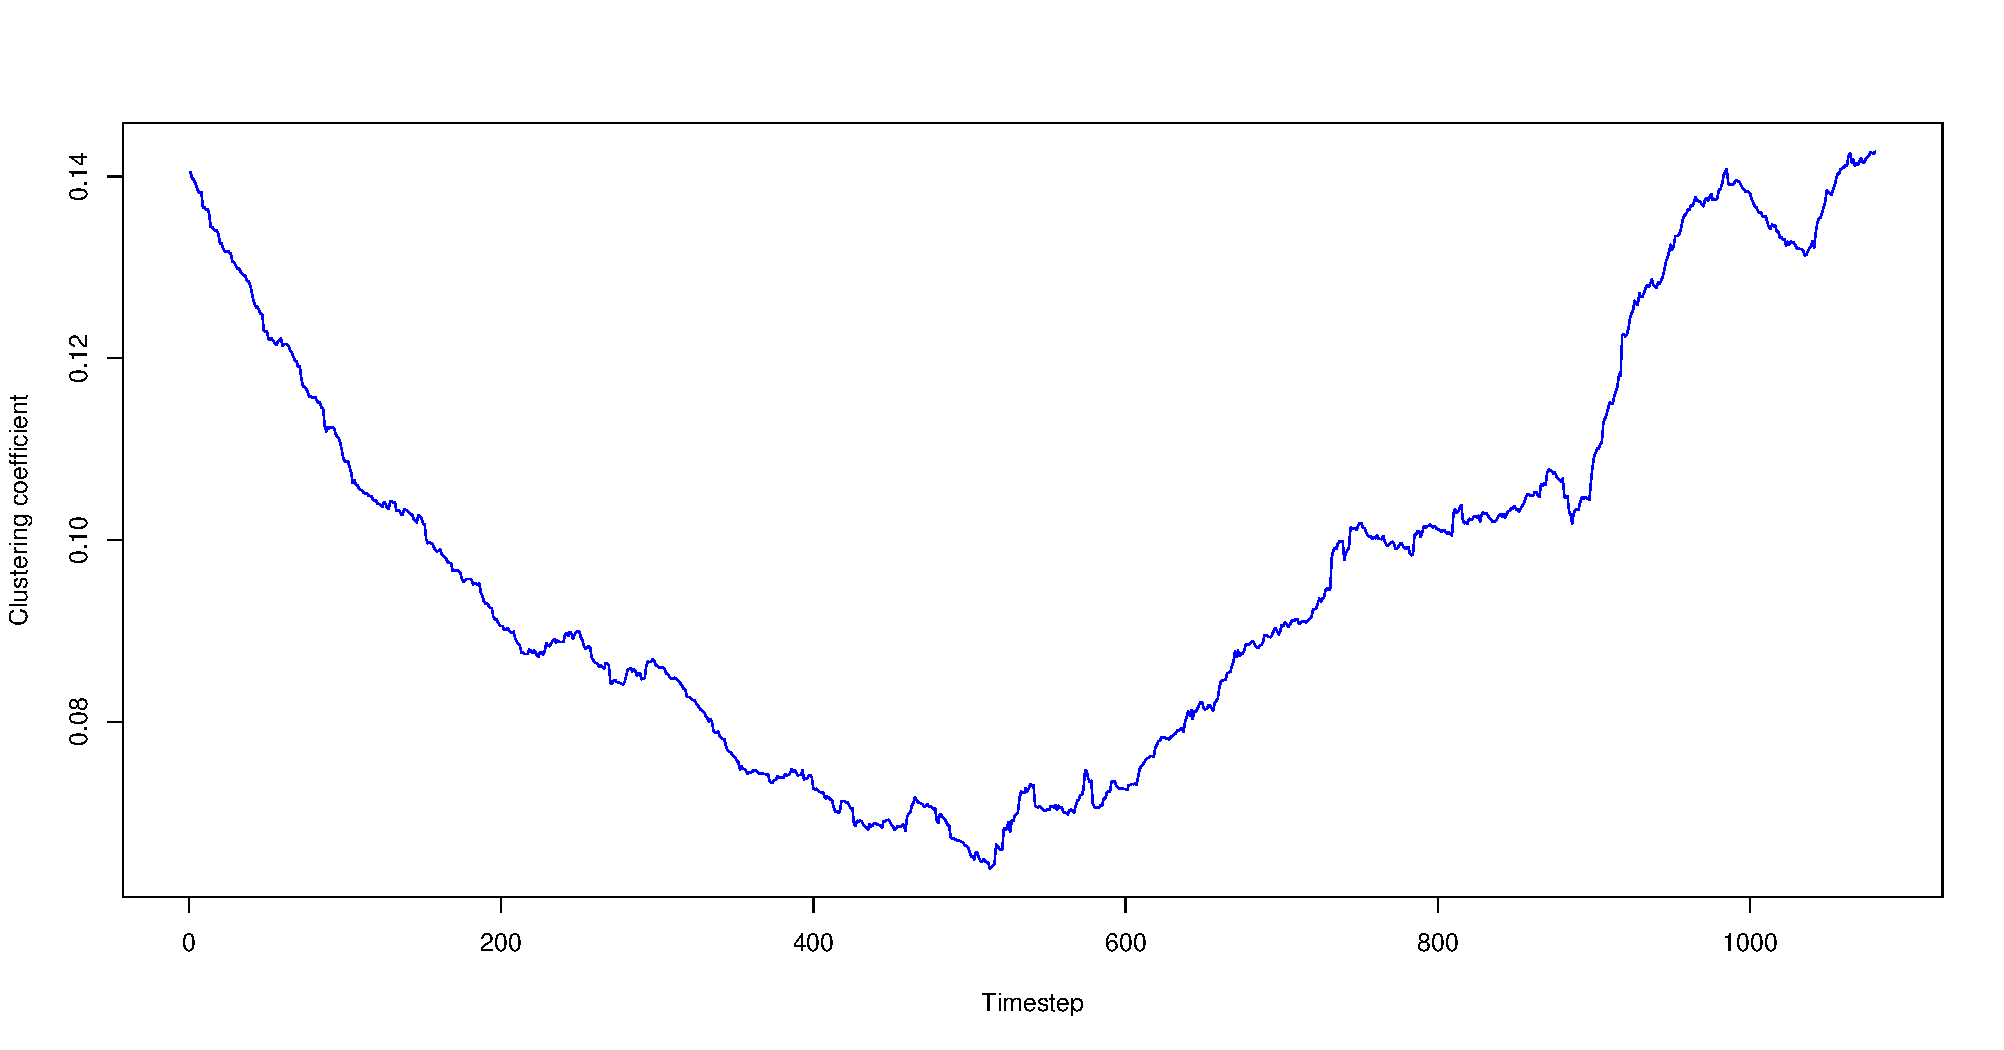
\includegraphics[width=83mm]{images/clustering_1000_sf_1080_0.pdf} \\
a. Densità & b. Coefficiente di clustering \\[6pt]
 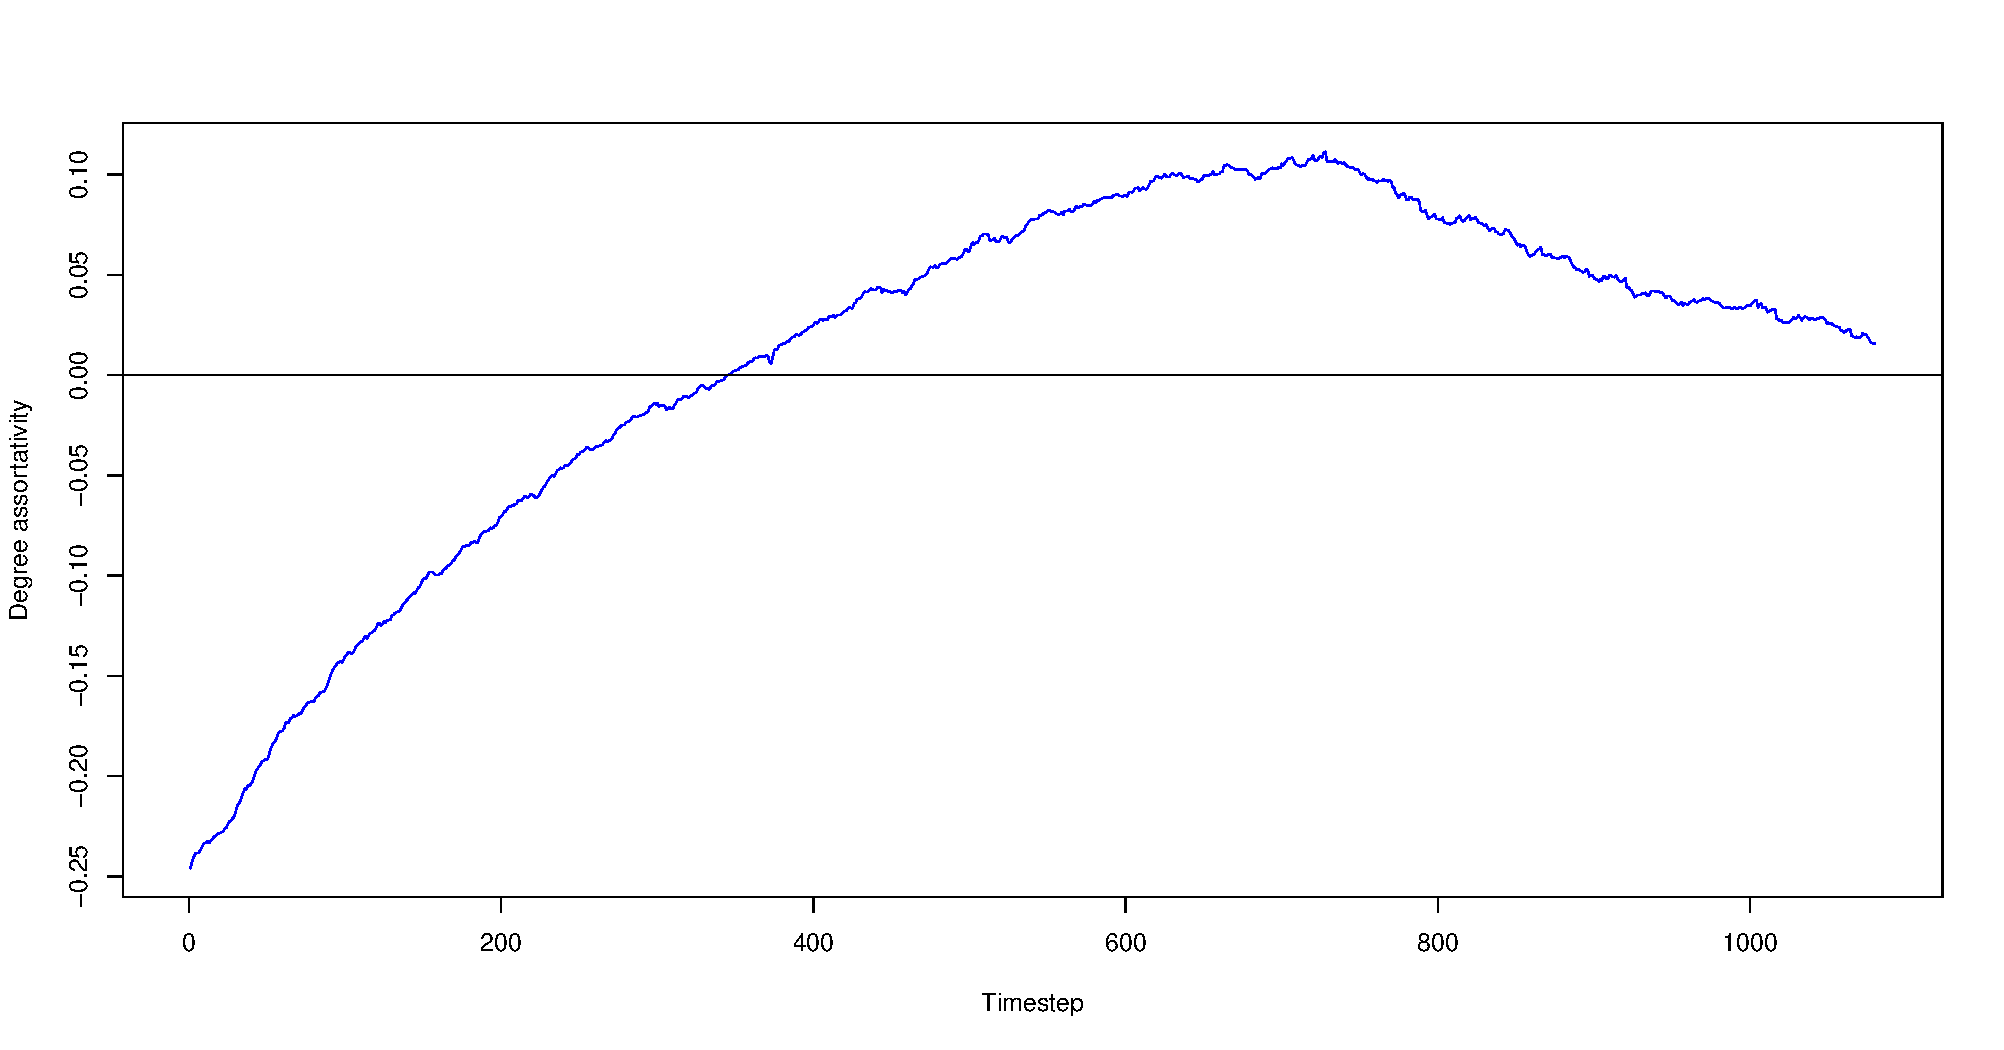
\includegraphics[width=83mm]{images/deg_assortativity_1000_sf_1080_0.pdf} &   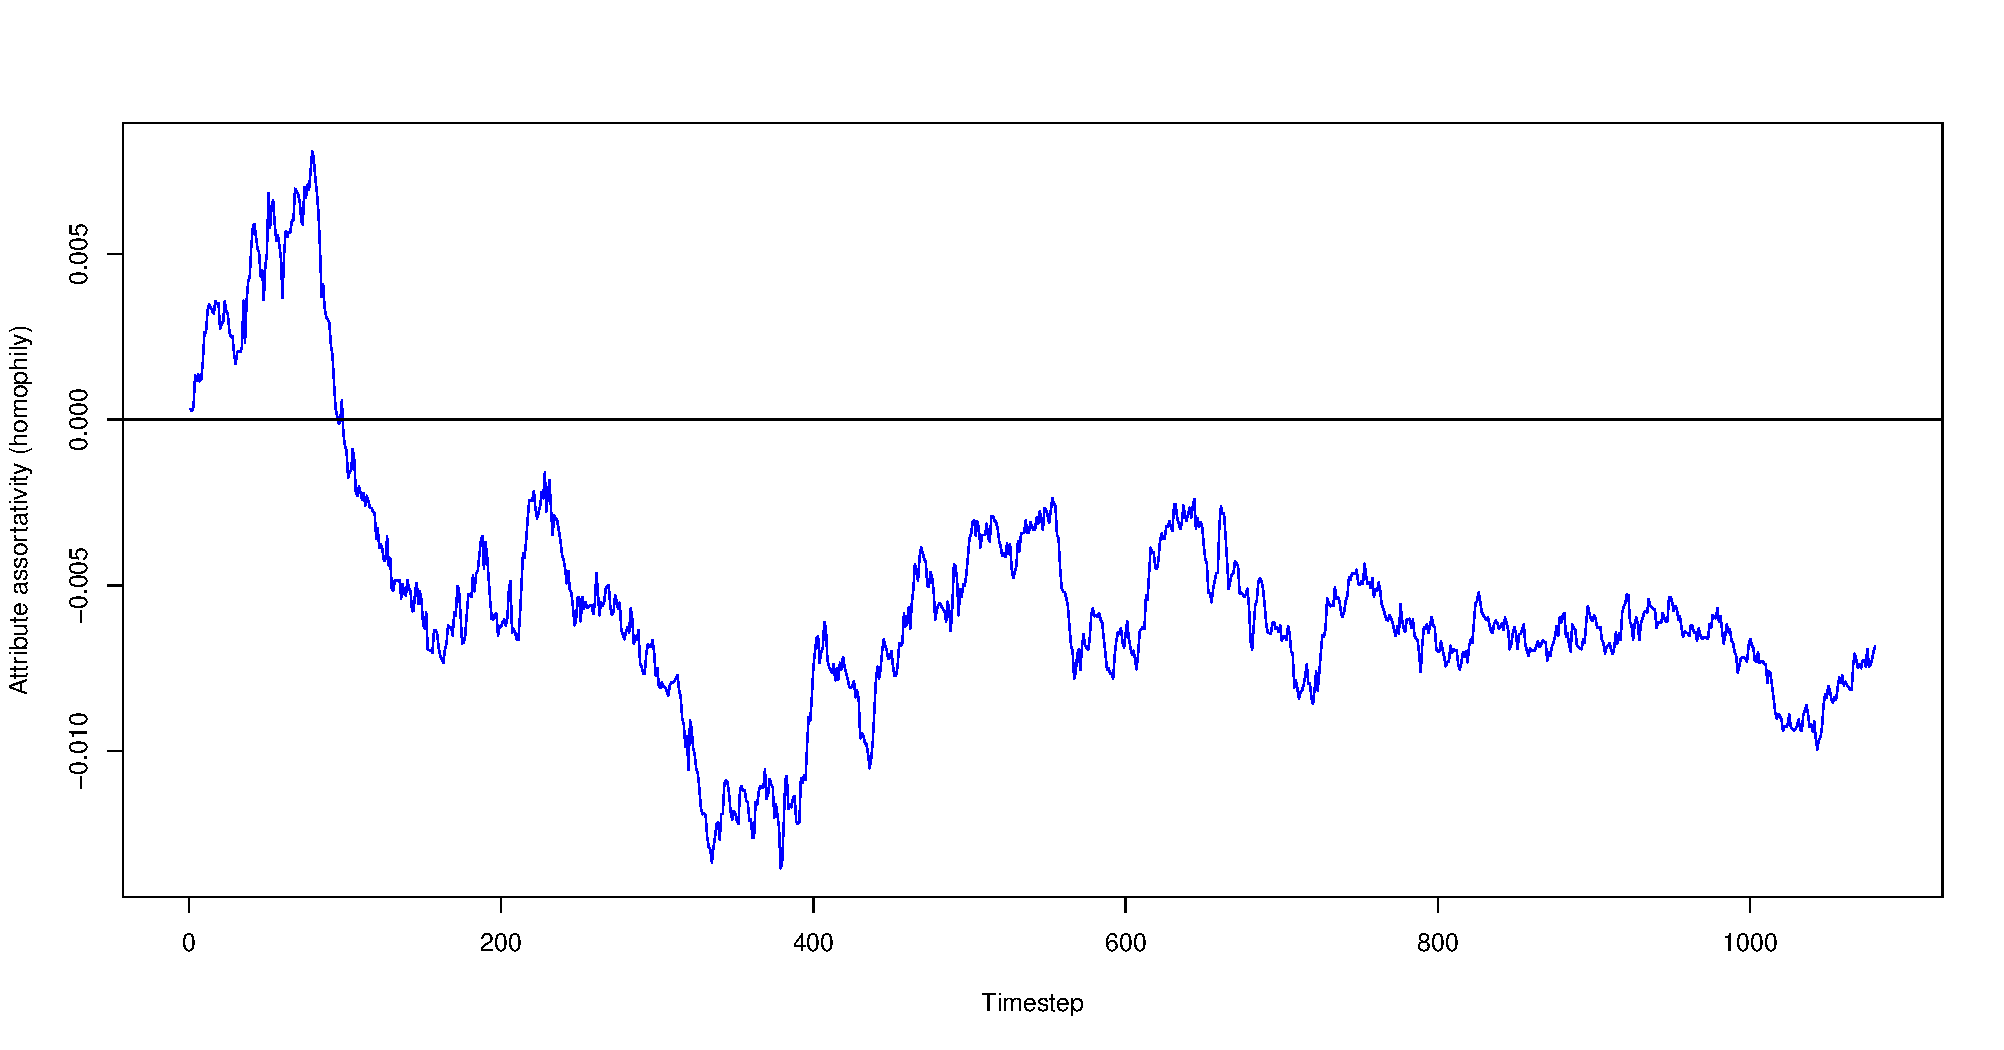
\includegraphics[width=83mm]{images/homophily_1000_sf_1080_0.pdf} \\
c. Assortatività per grado & d. Assortatività per attributo \\[6pt]
\end{tabular}
\caption{Indici scale-free network, densità 0.1\%}
\label{fig:sf1}
\end{figure}
Nell'esperimento con istanziazione della rete iniziale a invarianza di scala (figura \ref{fig:sf1}) si può notare come la densità cresca in modo piuttosto contenuto sebbene in modo debolmente esponenziale: da una densità iniziale di circa $0.1\%$ si arriva a circa $0.5\%$. Il coefficiente di clustering invece ha un andamento particolare: decresce fino a poco prima della metà del periodo considerato, per poi iniziare una crescita irregolare fino alla fine dell'esperimento. Una spiegazione di questo fenomeno potrebbe essere il fatto che, in principio, la rete abbia molti nodi senza alcun collegamento in entrata o in uscita; inoltre, una porzione ancora maggiore di questi nodi ha solo pochi collegamenti in uscita verso i due, tre nodi ``hub" che fanno capo alla maggior parte degli archi. \'E plausibile quindi che, fino ad un certo punto, i collegamenti non vadano a rafforzare comunità già presenti, quanto a unire per la prima volta nodi distanti.
Al contrario, l'assortatività per grado cresce regolarmente fino all'iterazione 750 circa, per poi cominciare a calare leggermente: questo è indice del fatto che a partire da quel momento, l'in-degree medio dei nodi con molti collegamenti cresce in modo più rapido dell'out-degree dei nodi con pochi collegamenti, con effetto negativo sulla misura di assortatività \textit{r(out,in)}. Questo dovrebbe essere indicatore di una tendenza della rete a conservare una configurazione ad invarianza di scala.\\
A differenza degli altri indici, l'assortatività per attributo è molto irregolare: dopo un brusco calo che la porta ad assumere valori negativi, continua ad oscillare in prossimità dello zero, senza mai tornare a valori positivi. Questo è segno che i nodi tendono a formare legami a prescindere dal 
\begin{figure}[t]
\begin{tabular}{cc}
  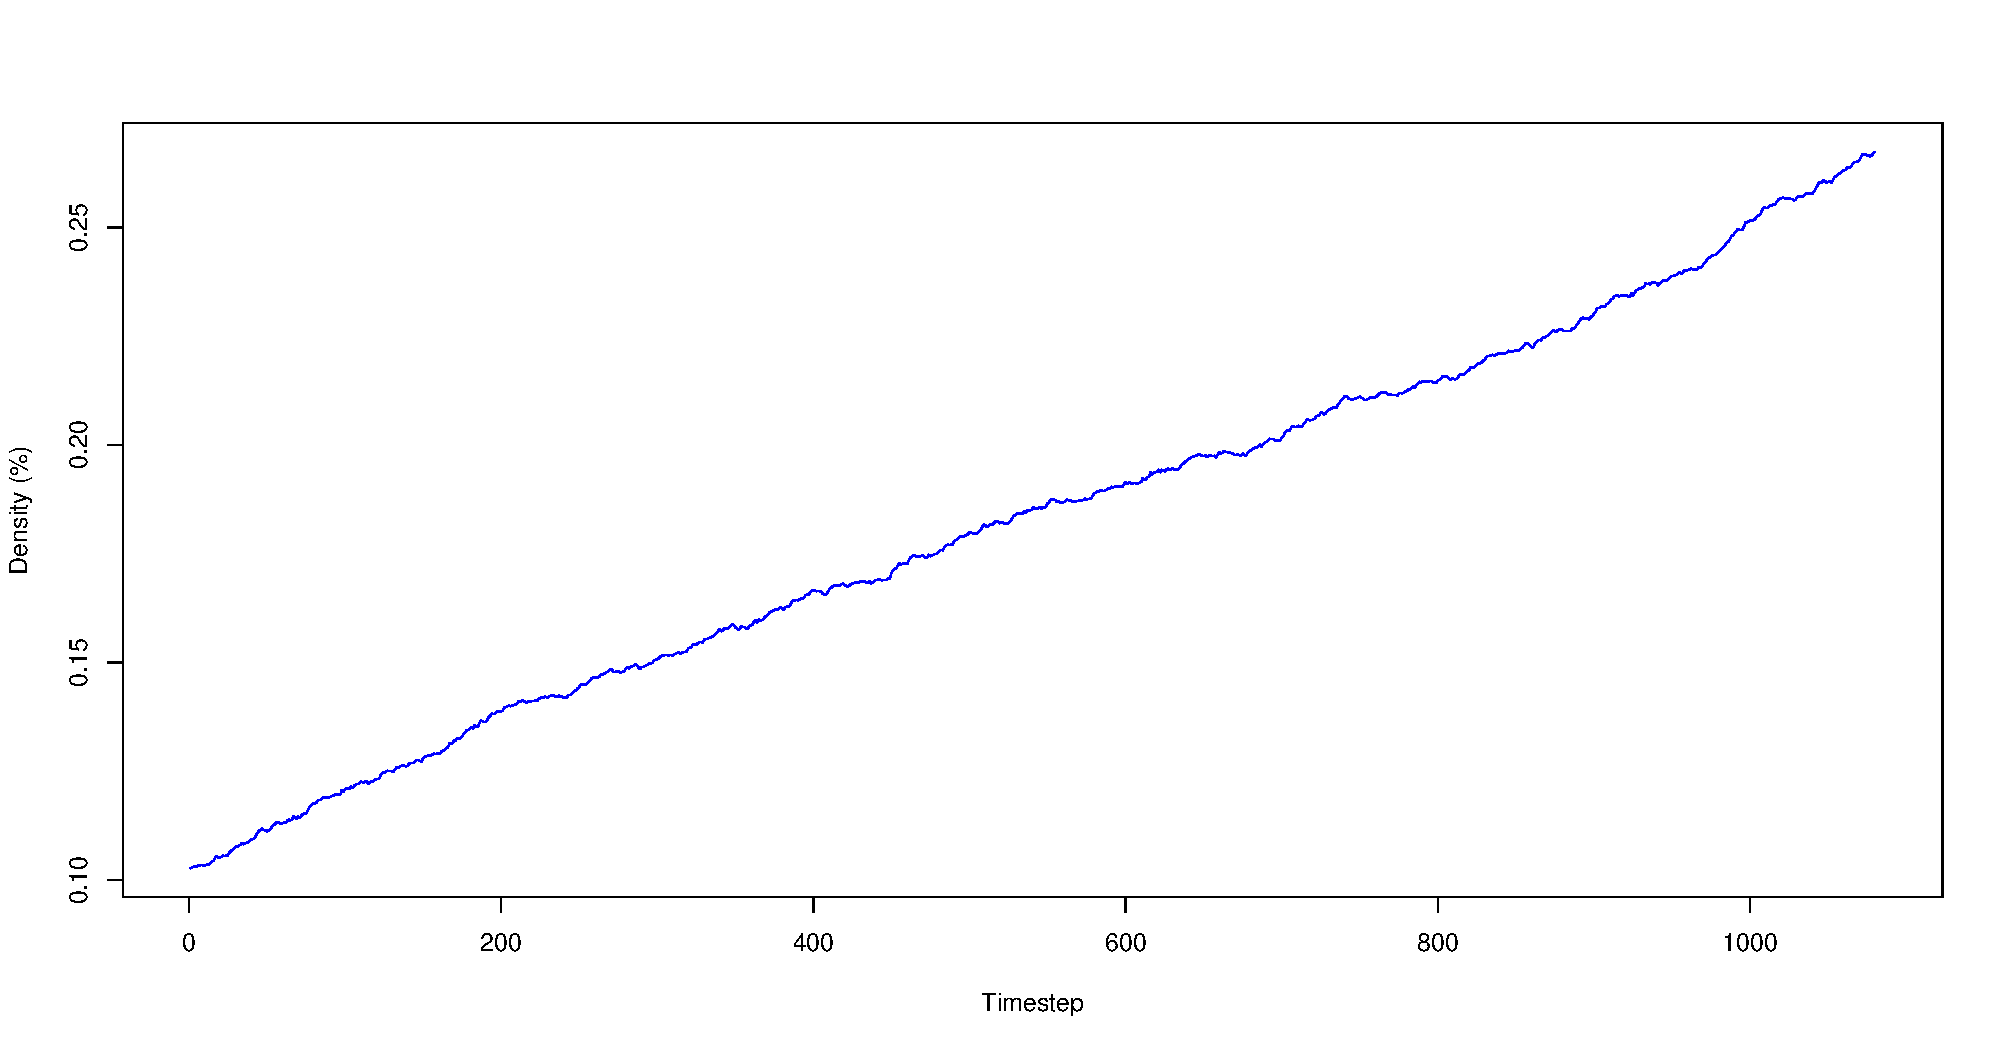
\includegraphics[width=83mm]{images/evolution_1000_rnd_1080_01_0.pdf} &   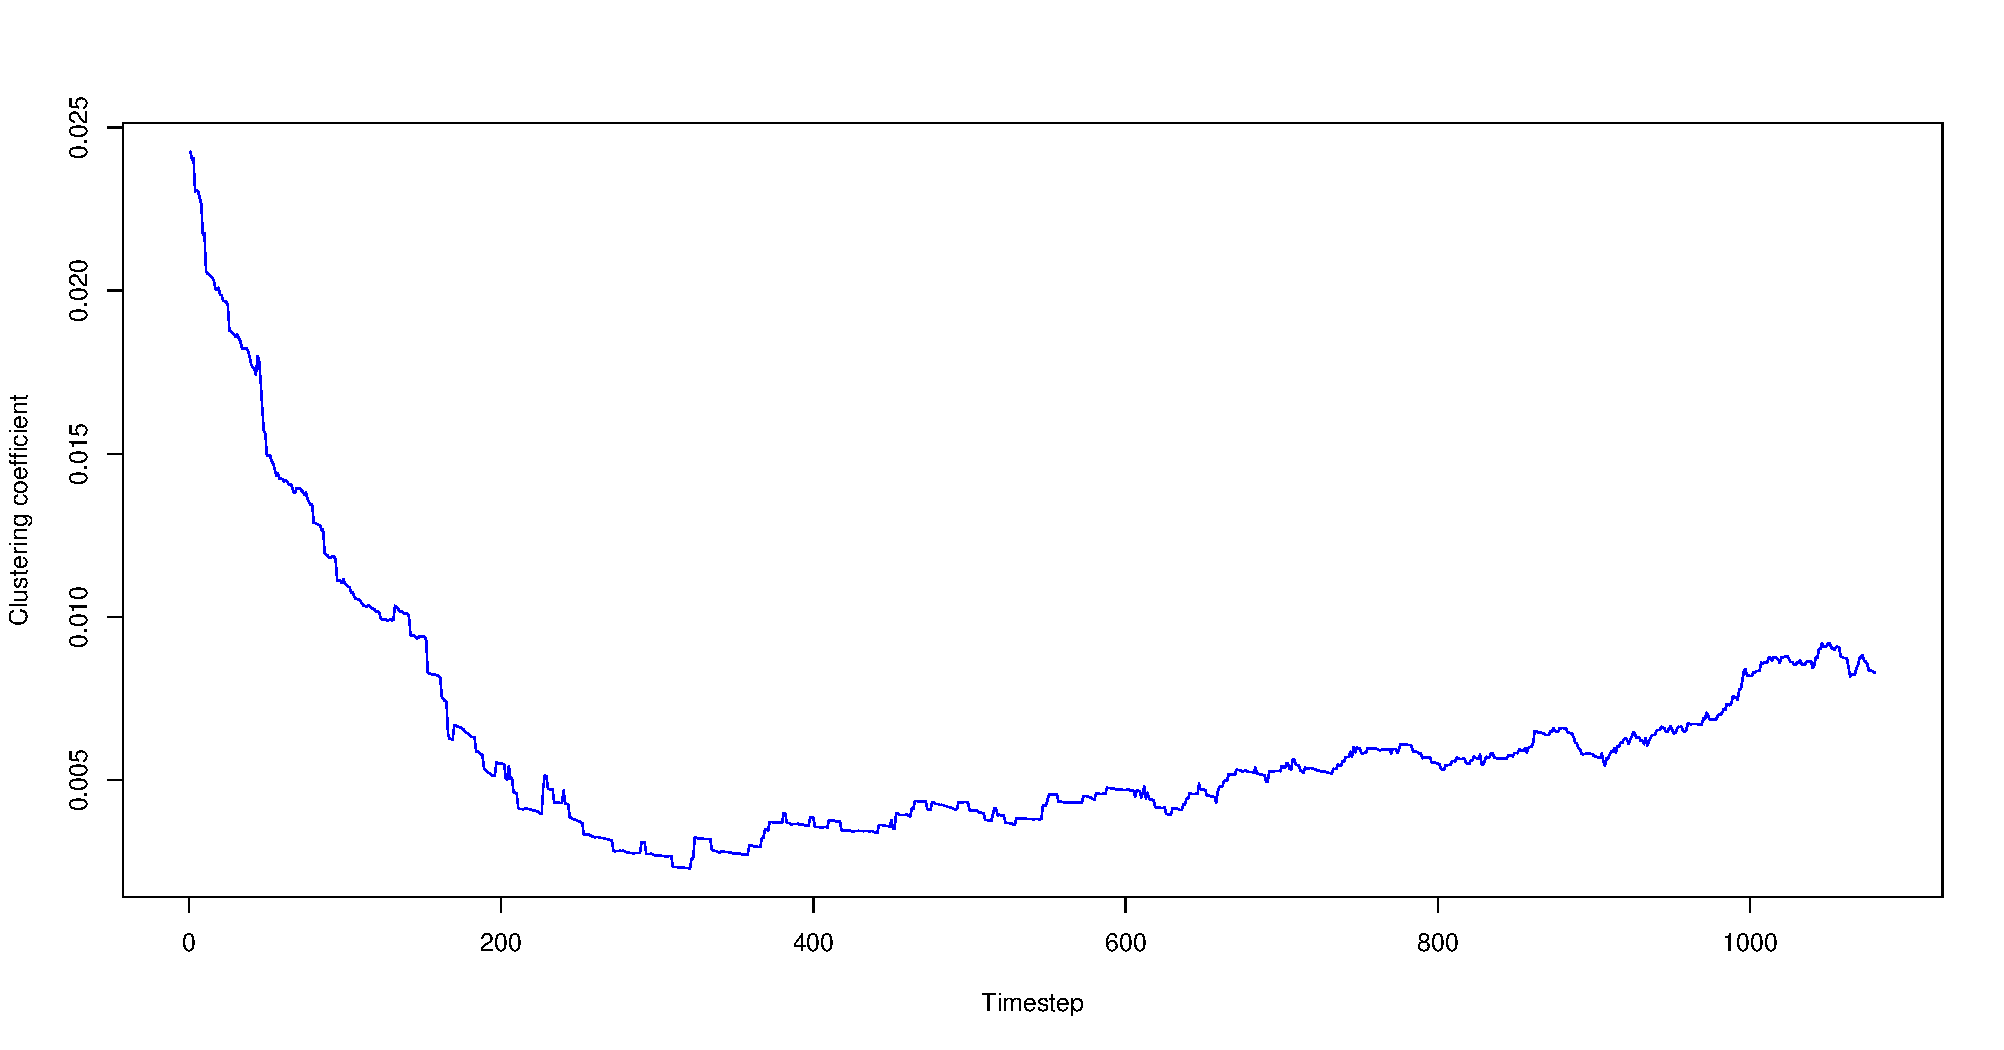
\includegraphics[width=83mm]{images/clustering_1000_rnd_1080_01_0.pdf} \\
a. Densità & b. Coefficiente di clustering \\[6pt]
 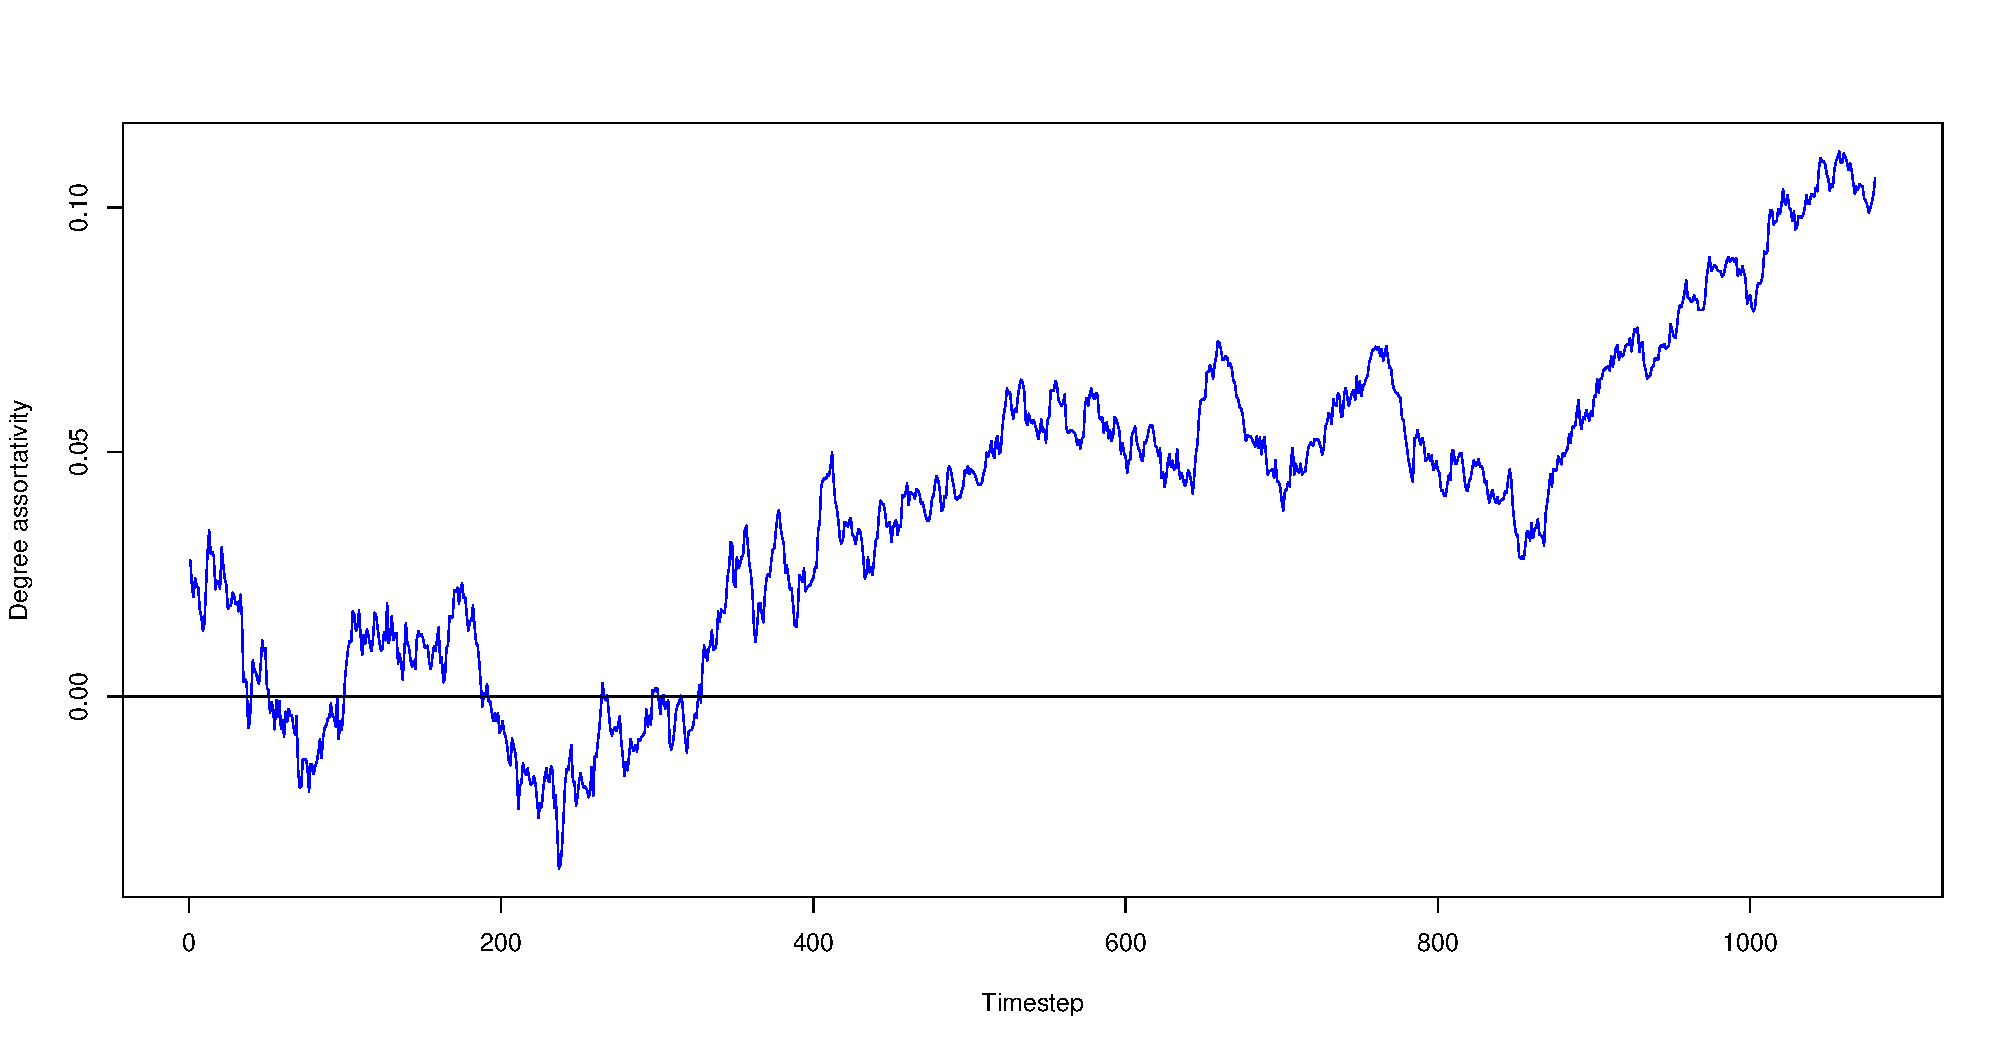
\includegraphics[width=83mm]{images/deg_assortativity_1000_rnd_1080_01_0.pdf} &   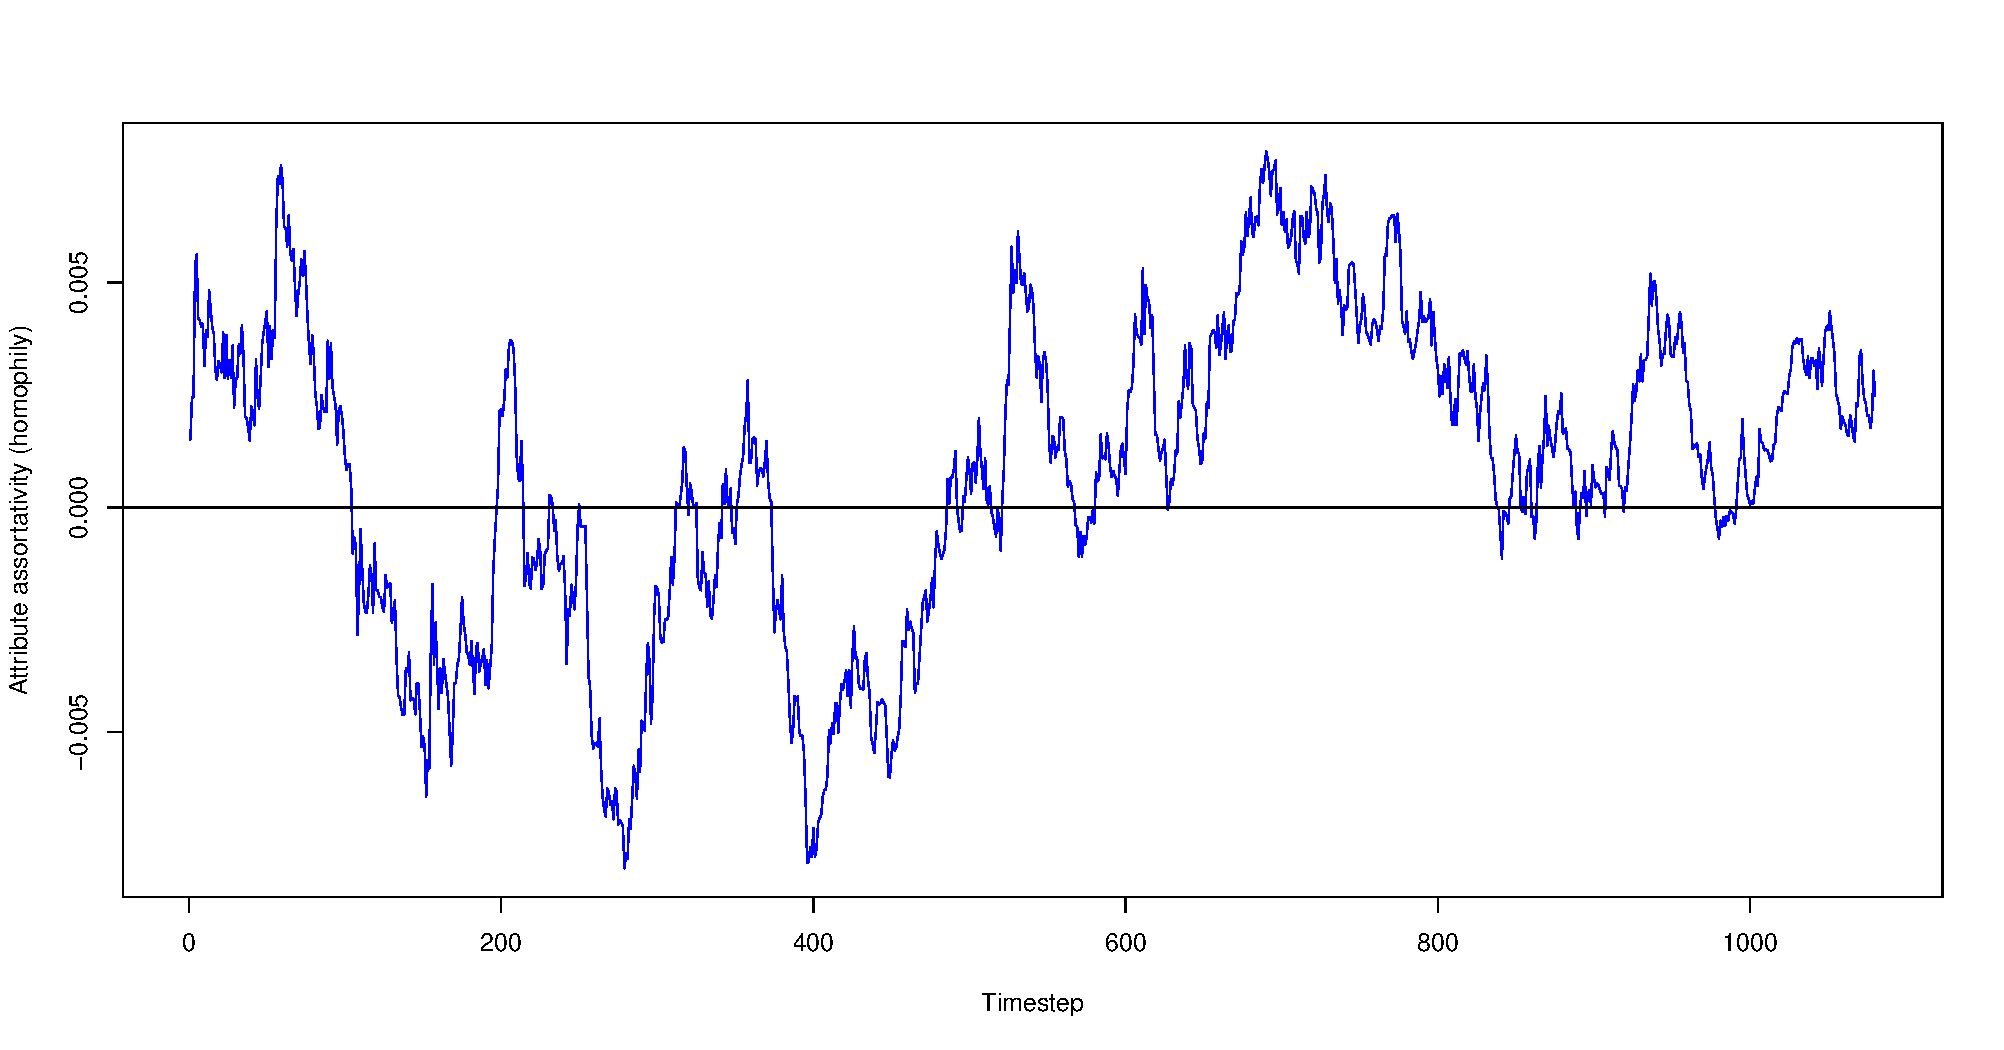
\includegraphics[width=83mm]{images/homophily_1000_rnd_1080_01_0.pdf} \\
c. Assortatività per grado & d. Assortatività per attributo \\[6pt]
\end{tabular}
\centering
\caption{Indici random network, densità 0.1\%}
\label{fig:rnd01}
\end{figure}
topic più rappresentativo di ognuno.\\ \\
L'esperimento successivo (figura \ref{fig:rnd01}) condivide con il primo il valore di densità iniziale, mentre differisce per costruzione: è infatti una random network priva, quindi, di nodi ``hub"; si riscontrano comunque nodi con più collegamenti in entrata e in uscita rispetto agli altri, ma la differenza, in questi termini, è molto ridotta. Ciò si rispecchia in una crescita molto più contenuta e lineare della densità (si arriva all'ultima iterazione con circa lo $0.3\%$), con i nodi che, avendo tutti un \textit{field of view} limitato, fanno fatica a stabilire nuovi collegamenti con nodi affini dal punto di vista degli interessi. Da qui si può trarre la conclusione che la presenza di nodi ``popolari" faciliti l'instaurazione di nuovi legami tra nodi meno importanti.
Inoltre, nell'andamento del coefficiente di clustering, si riscontra lo stesso fenomeno osservato in precedenza sulla scale-free network: dopo un calo iniziale, l'indice torna a crescere, ma in modo sensibilmente più lento rispetto all'altro caso. Da notare anche il valore di partenza, circa cinque volte minore. Anche questo comportamento può essere imputato alla scarsa densità e all'elevata sparsità degli archi, per cui le comunità vengono costituite con fatica. L'assortatività per grado mostra un andamento incerto ma crescente, a indicare che i nodi tendono a legarsi in base alla similarità tra out e in degree. L'assortatività per attributo è più incerta rispetto al caso precedente, con la differenza che nella seconda metà della simulazione rimane quasi sempre positiva.
\begin{figure}[h]
\begin{tabular}{cc}
  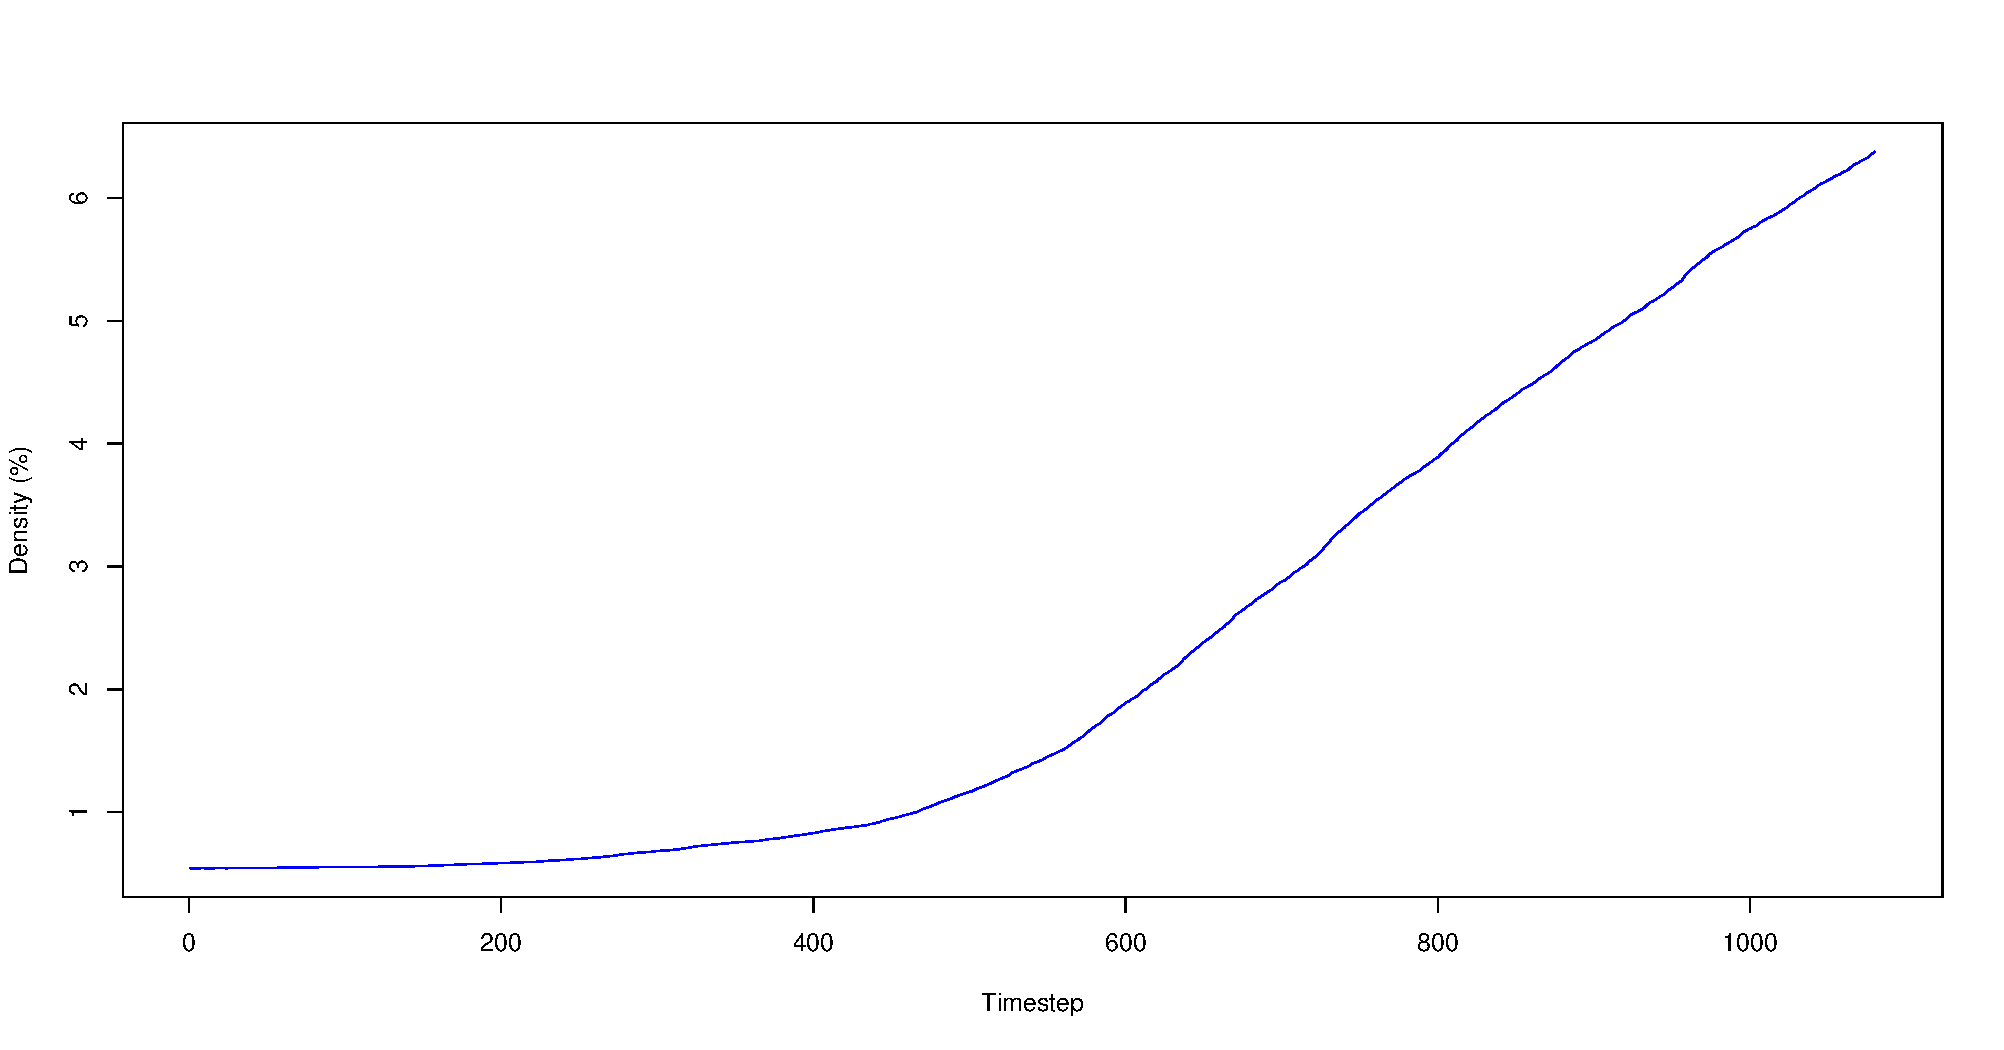
\includegraphics[width=81mm]{images/evolution_1000_rnd_1080_05_0.pdf} &   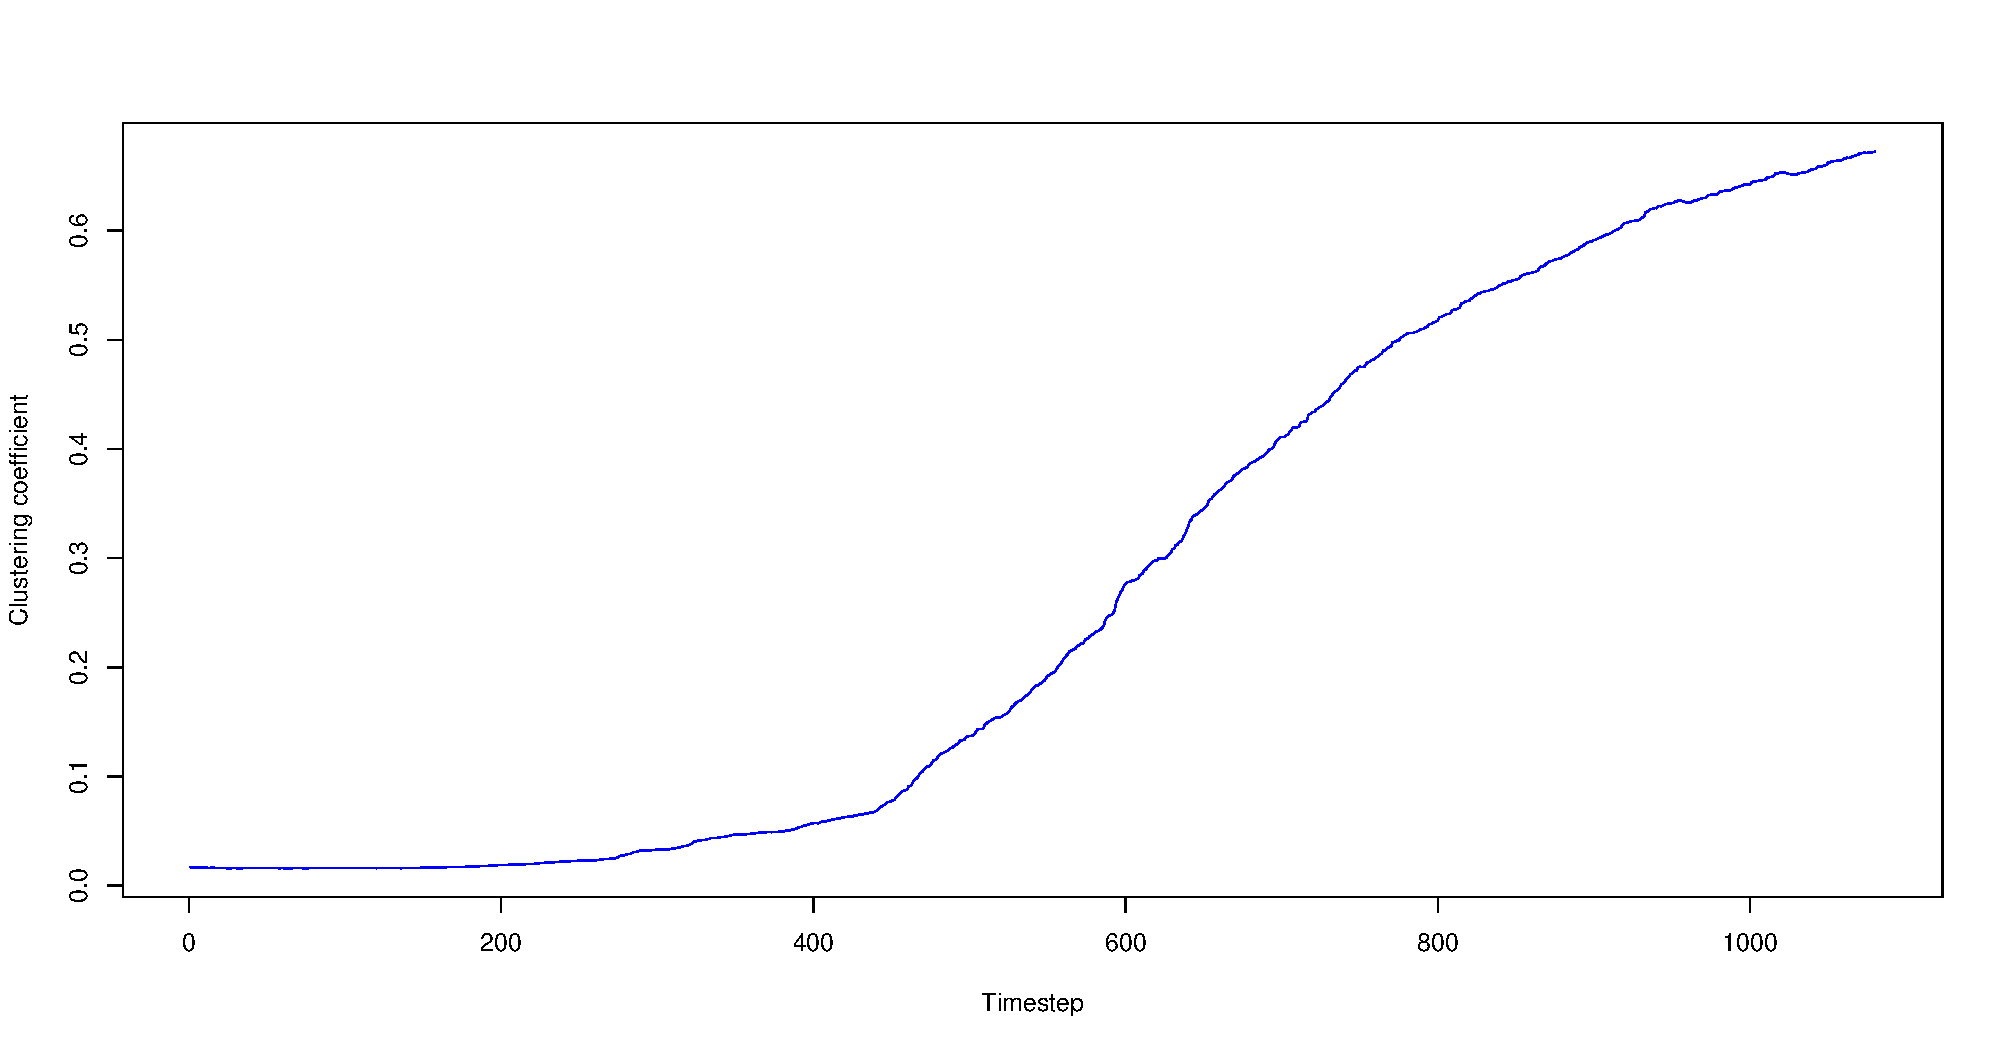
\includegraphics[width=81mm]{images/clustering_1000_rnd_1080_05_0.pdf} \\
a. Densità & b. Coefficiente di clustering \\[6pt]
 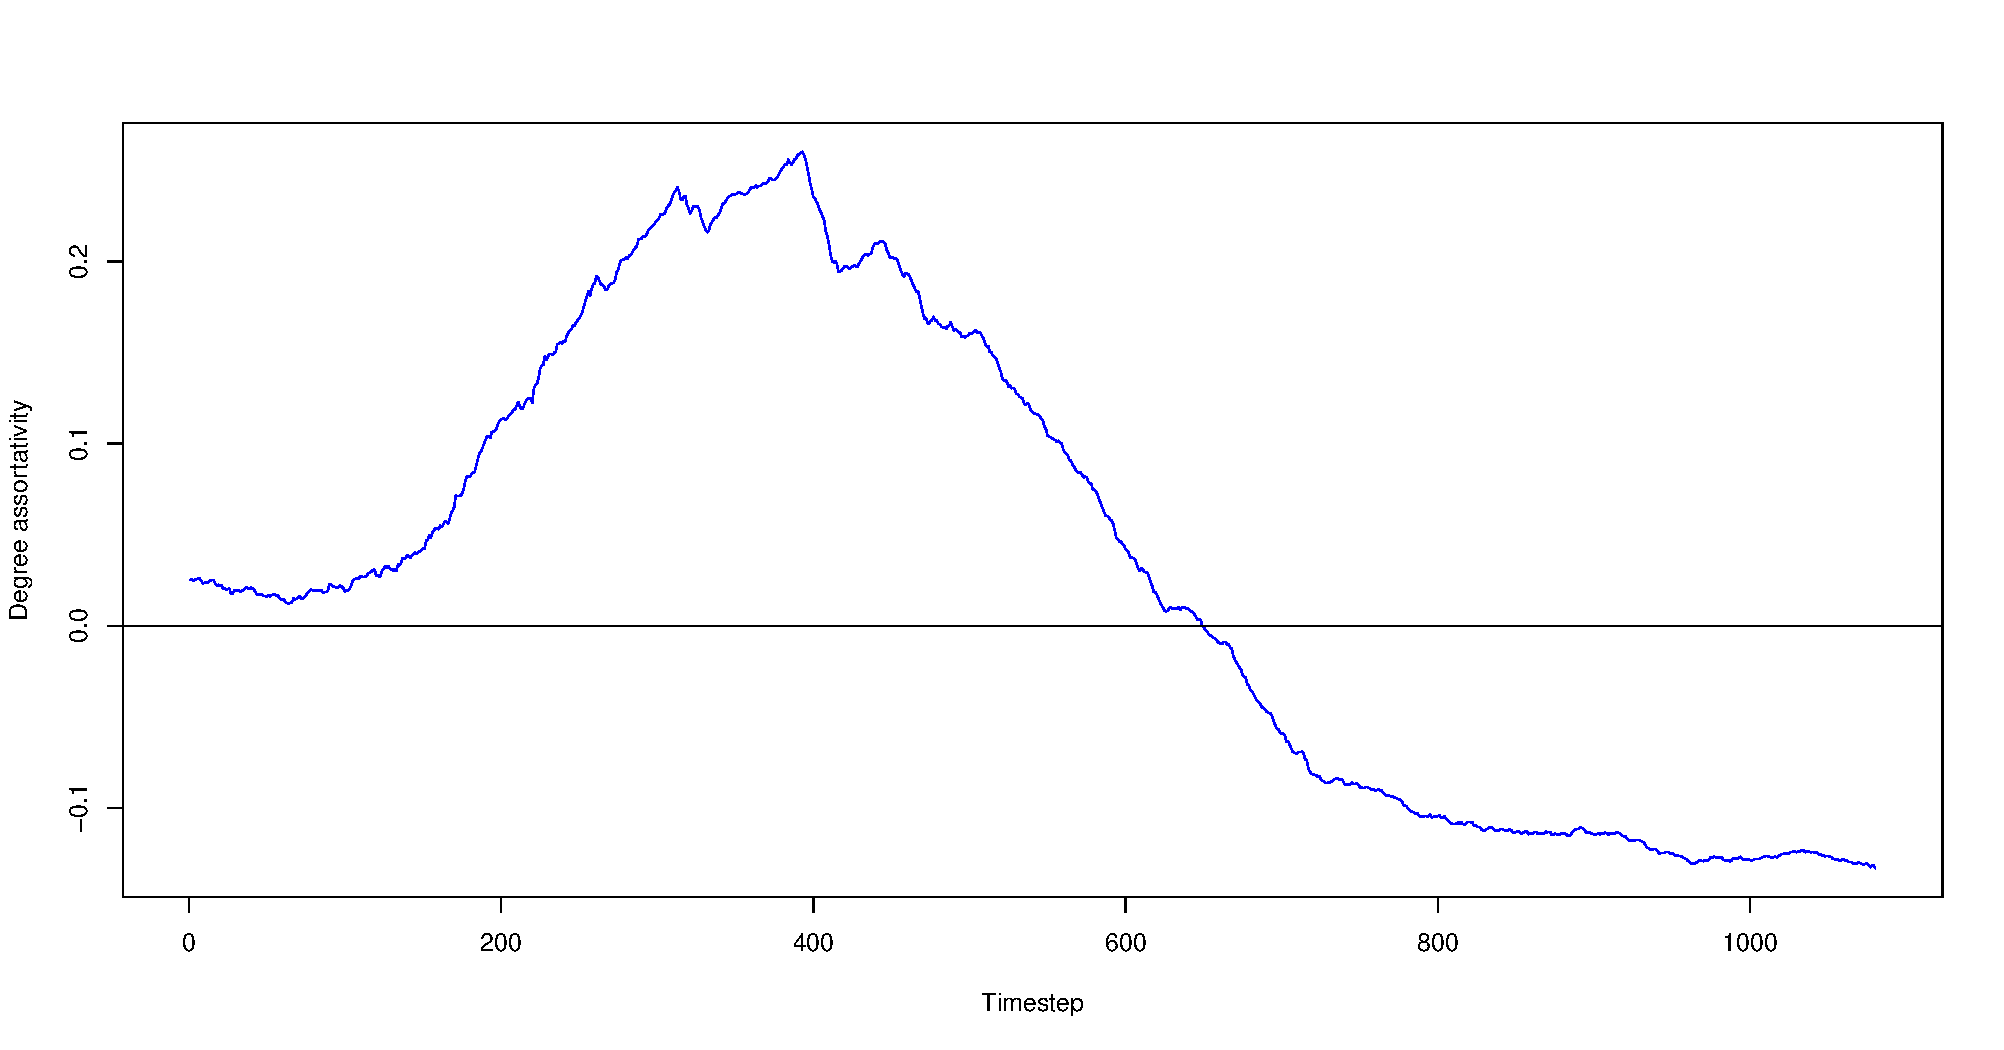
\includegraphics[width=81mm]{images/deg_assortativity_1000_rnd_1080_05_0.pdf} &   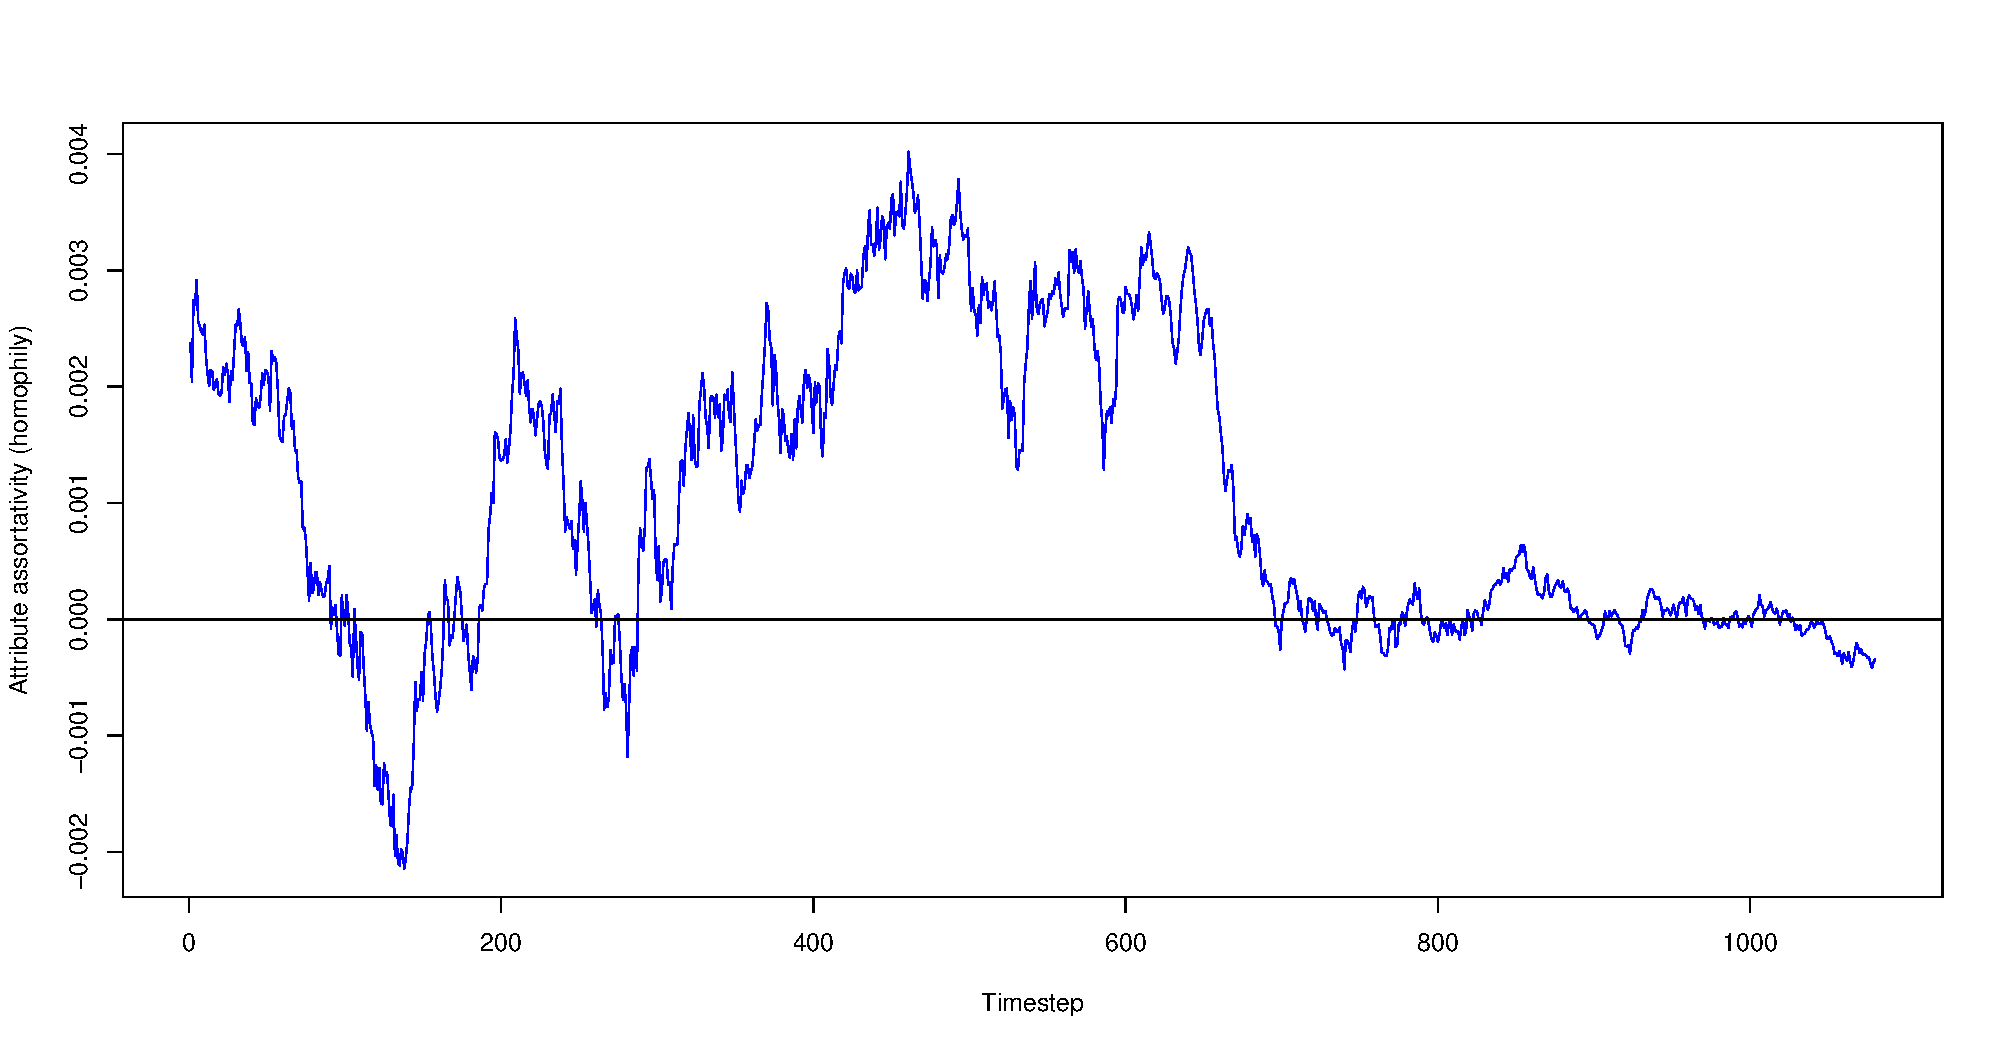
\includegraphics[width=81mm]{images/homophily_1000_rnd_1080_05_0.pdf} \\
c. Assortatività per grado & d. Assortatività per attributo \\[6pt]
\end{tabular}
\centering
\caption{Indici random network, densità 0.5\%}
\label{fig:rnd05}
\end{figure}
\\ \\Il caso con densità di partenza pari a $0.5\%$ (figura \ref{fig:rnd05}) è piuttosto interessante, in quanto vi abbiamo osservato la crescita più rapida per quanto riguarda la densità: dallo $0.5\%$ iniziale, dopo una fase relativamente calma, cresce fino a superare il $6\%$ alla fine della simulazione. Questo si riflette sugli altri indici: ad esempio, il coefficiente di clustering, dopo un rapido incremento con una pendenza pari a quella assunta dalla densità, comicia a ridurre l'ascesa. Questo suggerisce che, man mano che la densità si fa importante, i collegamenti avvengo sempre di più all'interno di comunità già formate. Non solo: a partire dall'iterazione 984 la rete ha anche raggiunto lo stato di completa \textit{connessione}, ovvero la rete è diventata un'unica componente connessa; questo concorre all'affievolimento della crescita del coefficiente di clustering, in quanto favorisce l'instaurazione di archi intra-comunità. Nell'assortatività per grado si ritrova il fenomeno osservato nella prima run: l'indice cresce fino a raggiungere un picco, per poi calare fino alla fine delle iterazioni, a indicare una tendenza della rete ad assumere una struttura ad invarianza di scala. Qui però il fenomeno è più rapido: il picco è più alto e viene raggiunto prima, mentre nella fase calante si verifica un livellamento improvviso, riscontrato anche nella misura di omofilia, dove l'assortatività per attributo si stabilizza sullo 0; questo comportamento può essere imputato al fatto che la rete ha raggiunto uno stato in cui le differenze tra i nodi, sia dal punto di vista della metrica $r(out,in)$ che dell'assortatività per attributo, sono meno accentuate; in altre parole, l'invarianza di scala comincia ad indebolirsi. Inoltre, la distanza tra i nodi diventa molto piccola, per cui è più facile per un agente scovare un altro agente simile per topic e instaurare un collegamento. 
\begin{figure}[H]
\begin{tabular}{cc}
  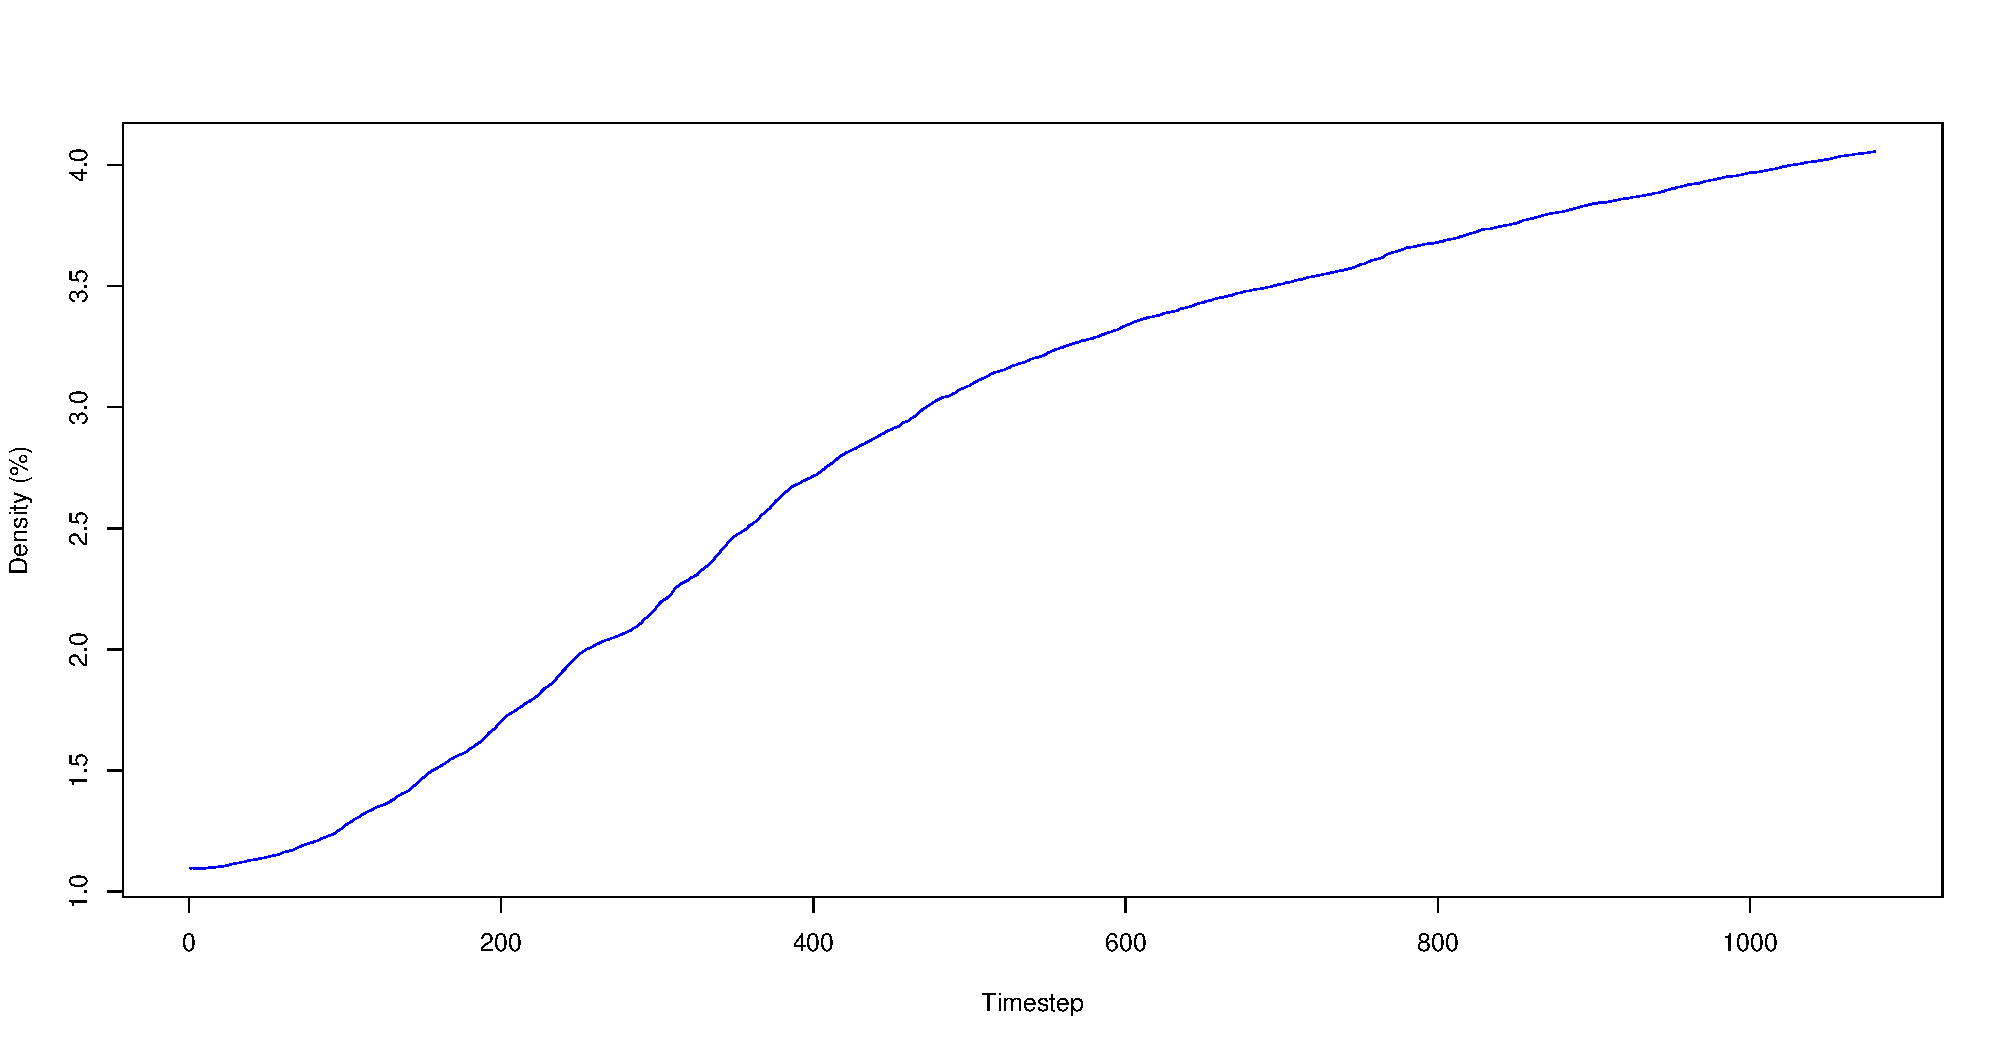
\includegraphics[width=81mm]{images/evolution_1000_rnd_1080_1_0.pdf} &   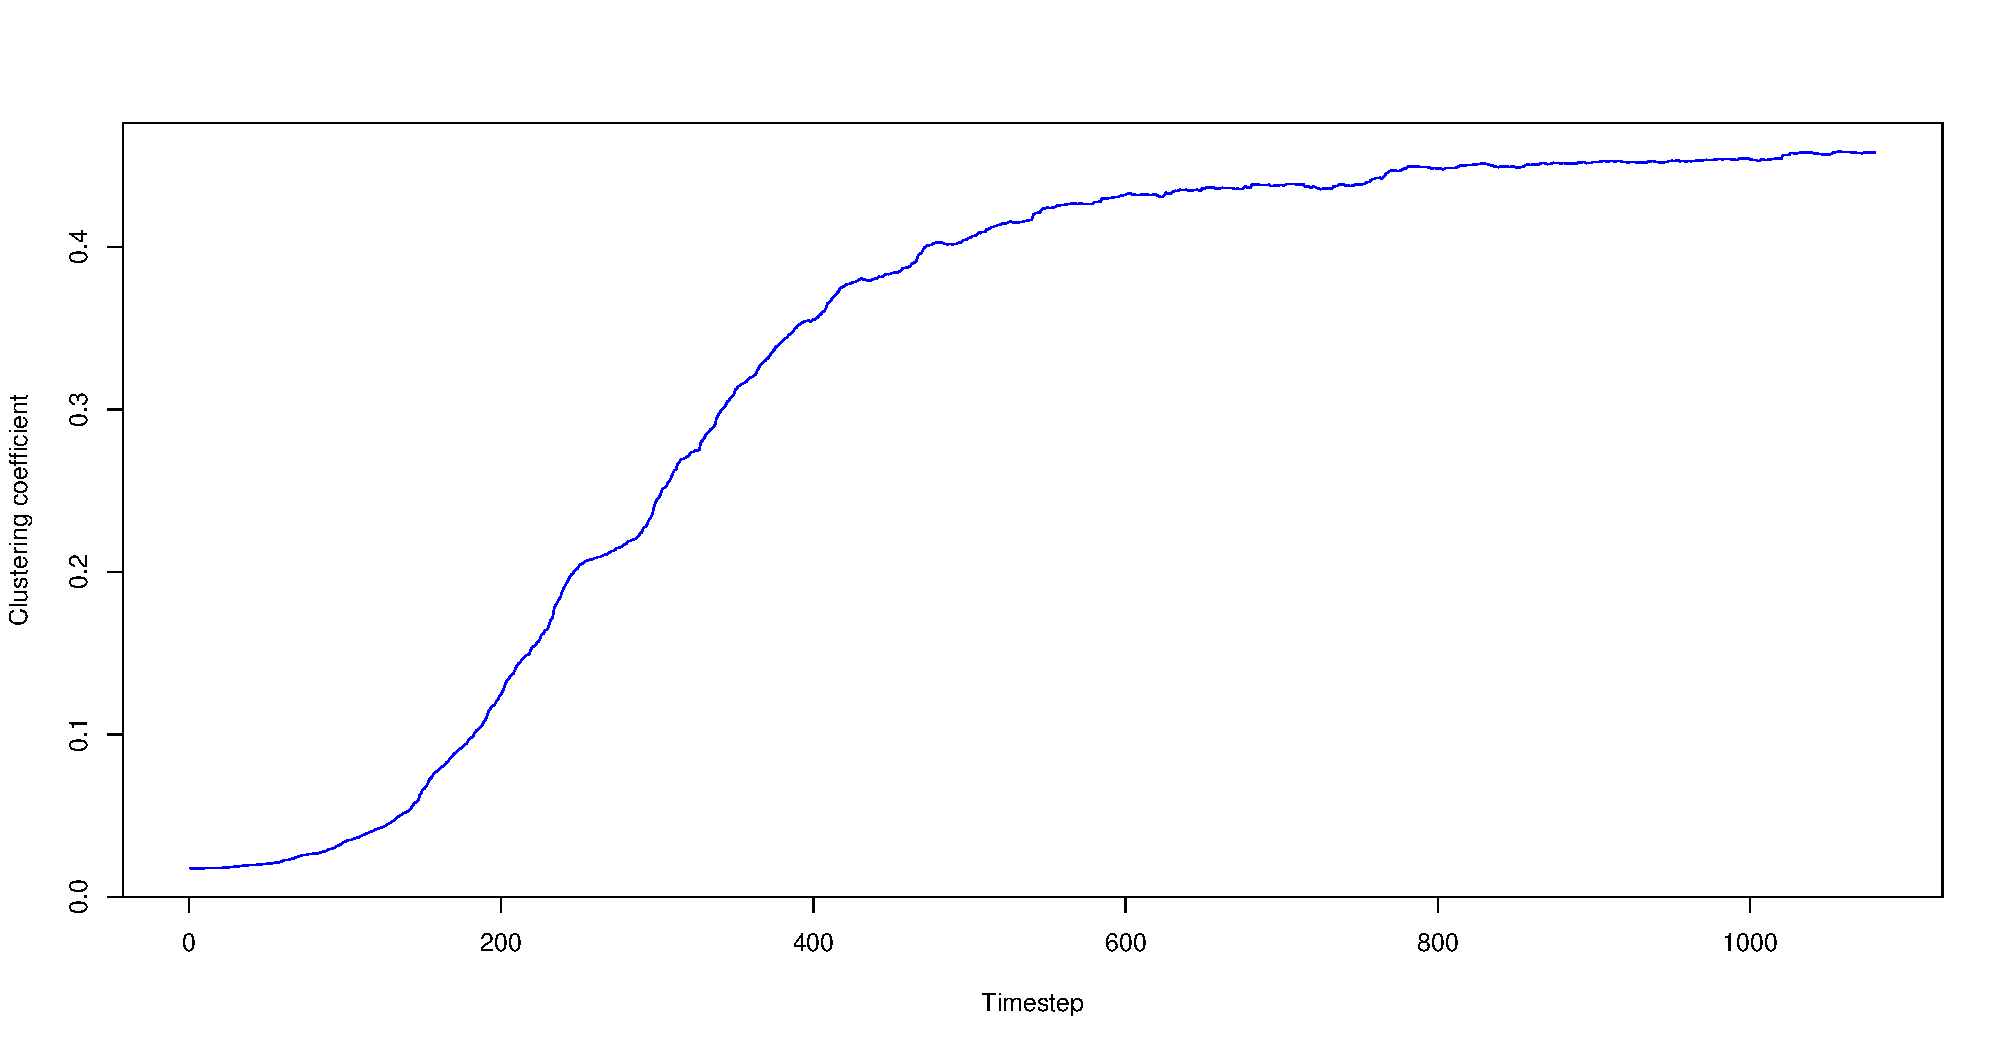
\includegraphics[width=81mm]{images/clustering_1000_rnd_1080_1_0.pdf} \\
a. Densità & b. Coefficiente di clustering \\[6pt]
 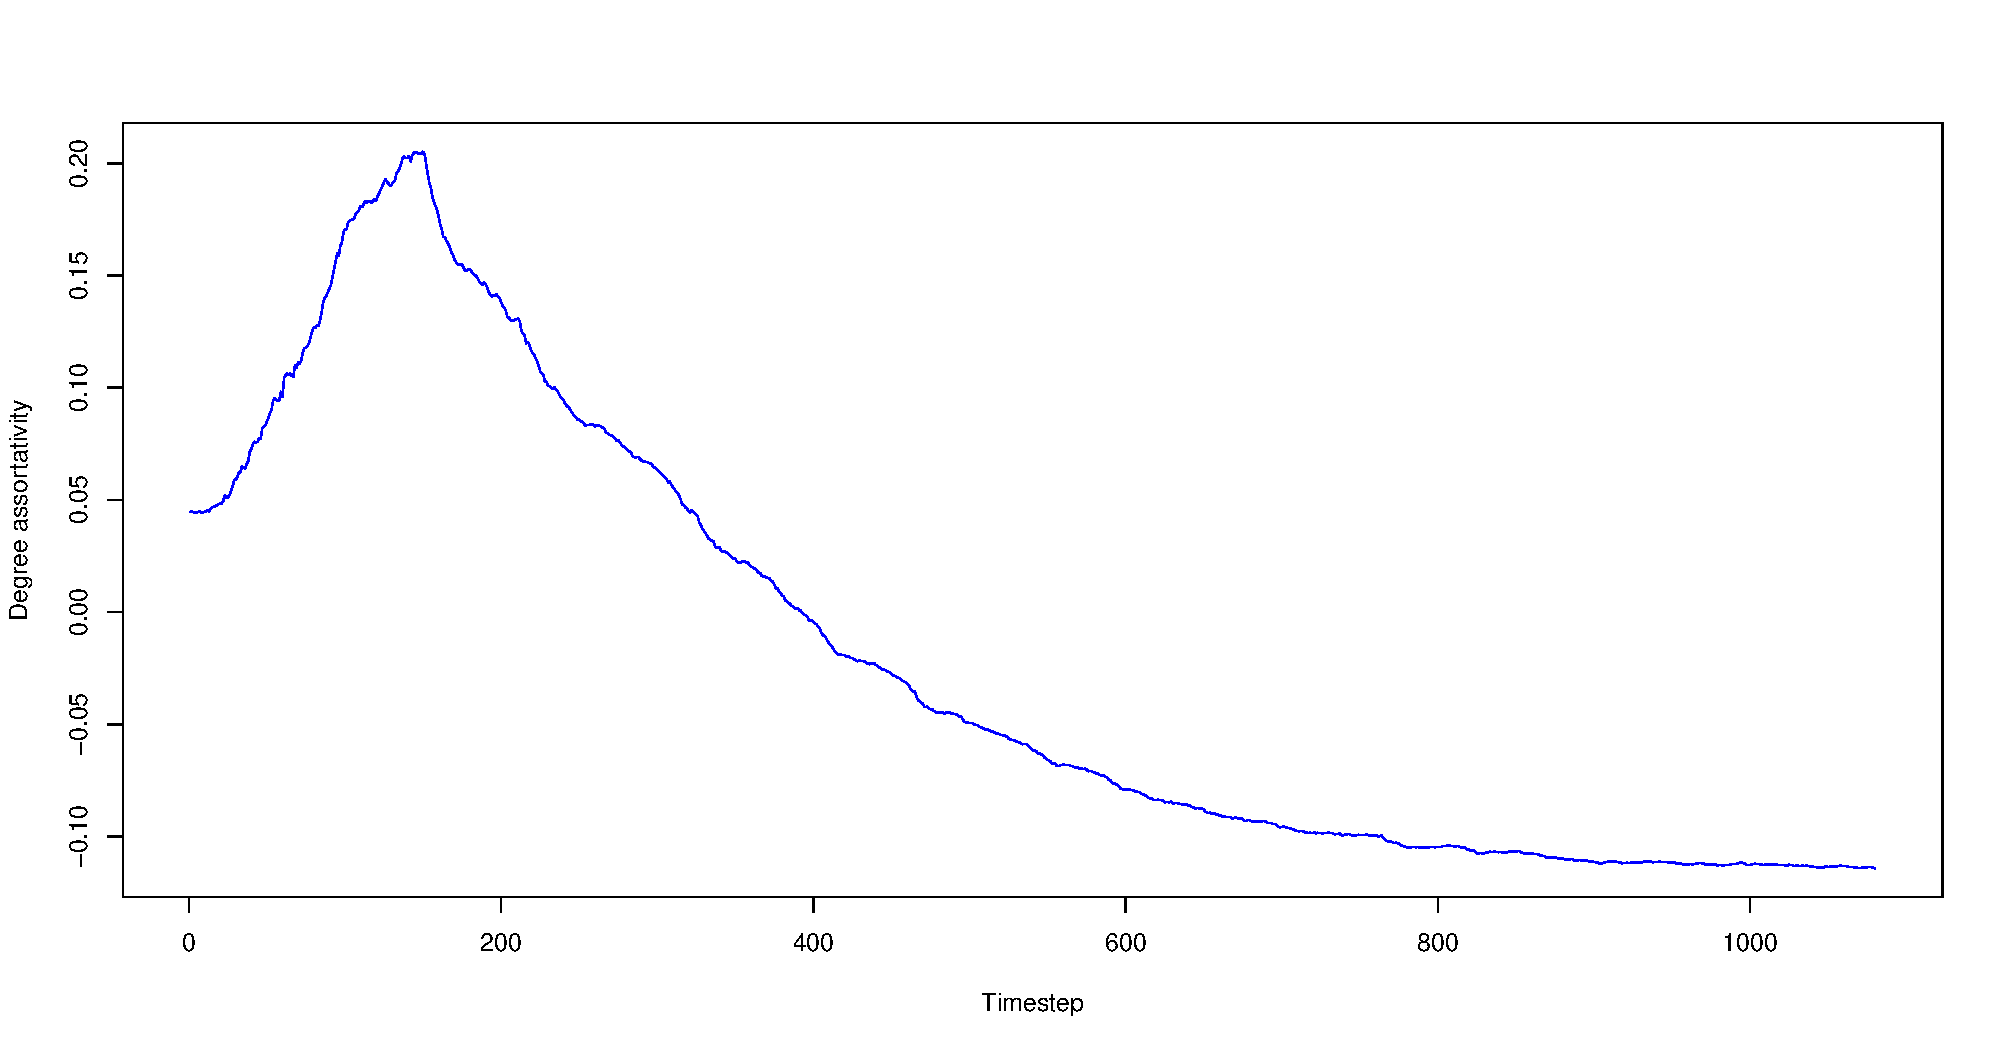
\includegraphics[width=81mm]{images/deg_assortativity_1000_rnd_1080_1_0.pdf} &   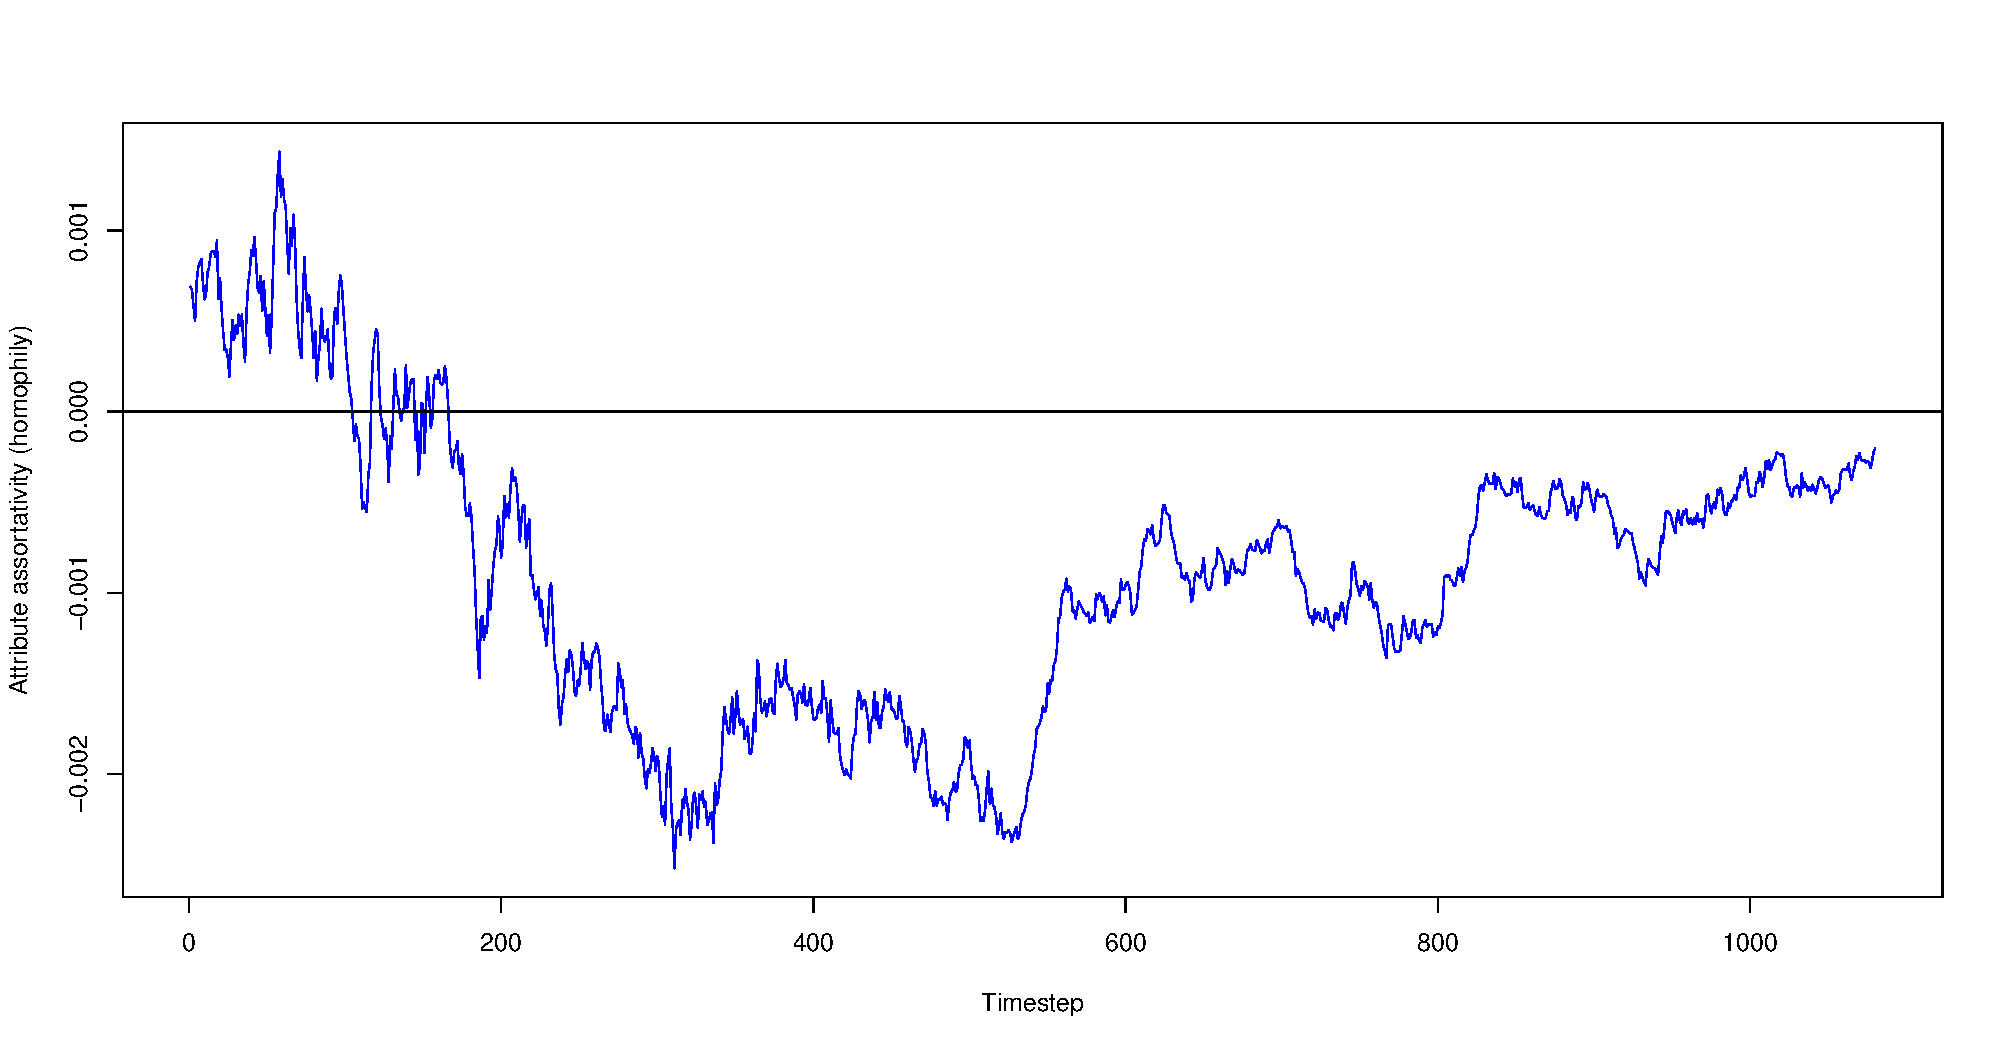
\includegraphics[width=81mm]{images/homophily_1000_rnd_1080_1_0.pdf} \\
c. Assortatività per grado & d. Assortatività per attributo \\[6pt]
\end{tabular}
\centering
\caption{Indici random network, densità 1.0\%}
\label{fig:rnd1}
%\end{figure}
%\begin{figure}[h]
\begin{tabular}{cc}
  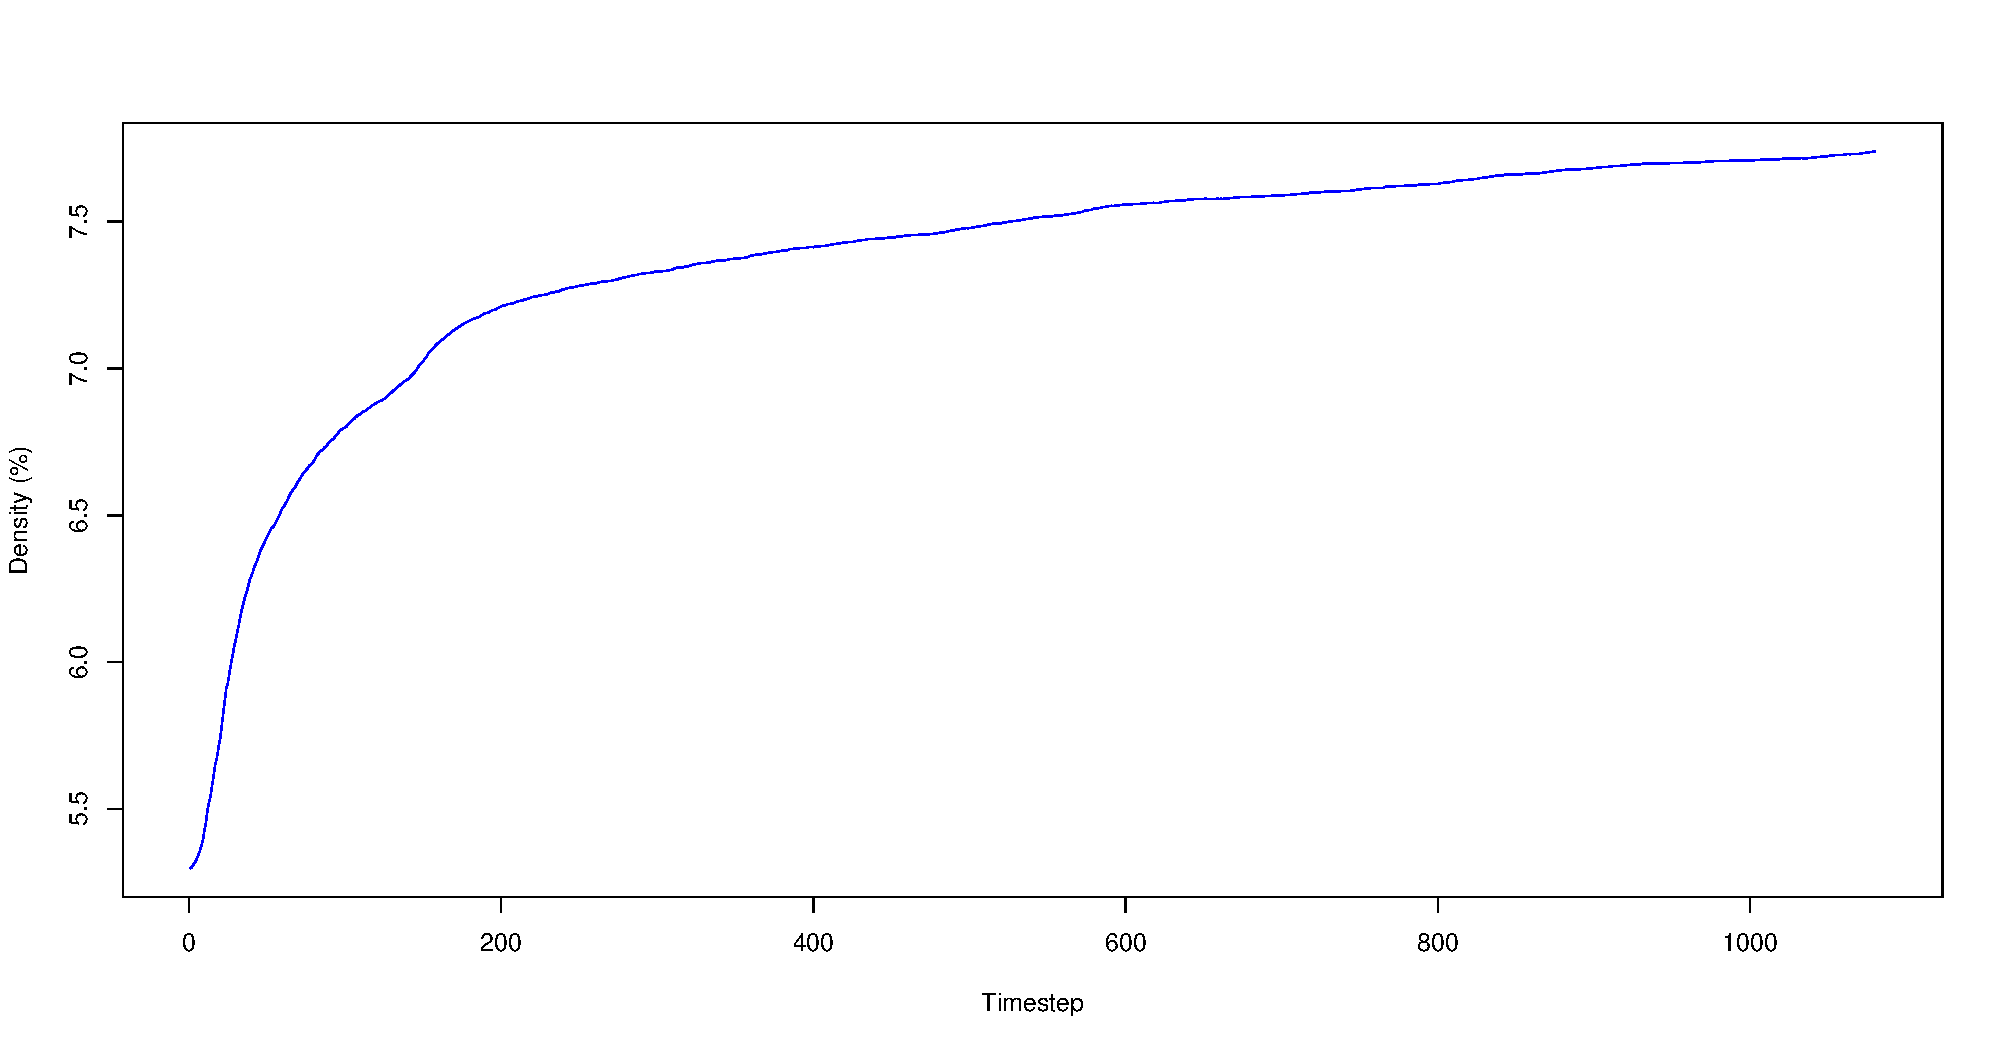
\includegraphics[width=81mm]{images/evolution_1000_rnd_1080_5_0.pdf} &   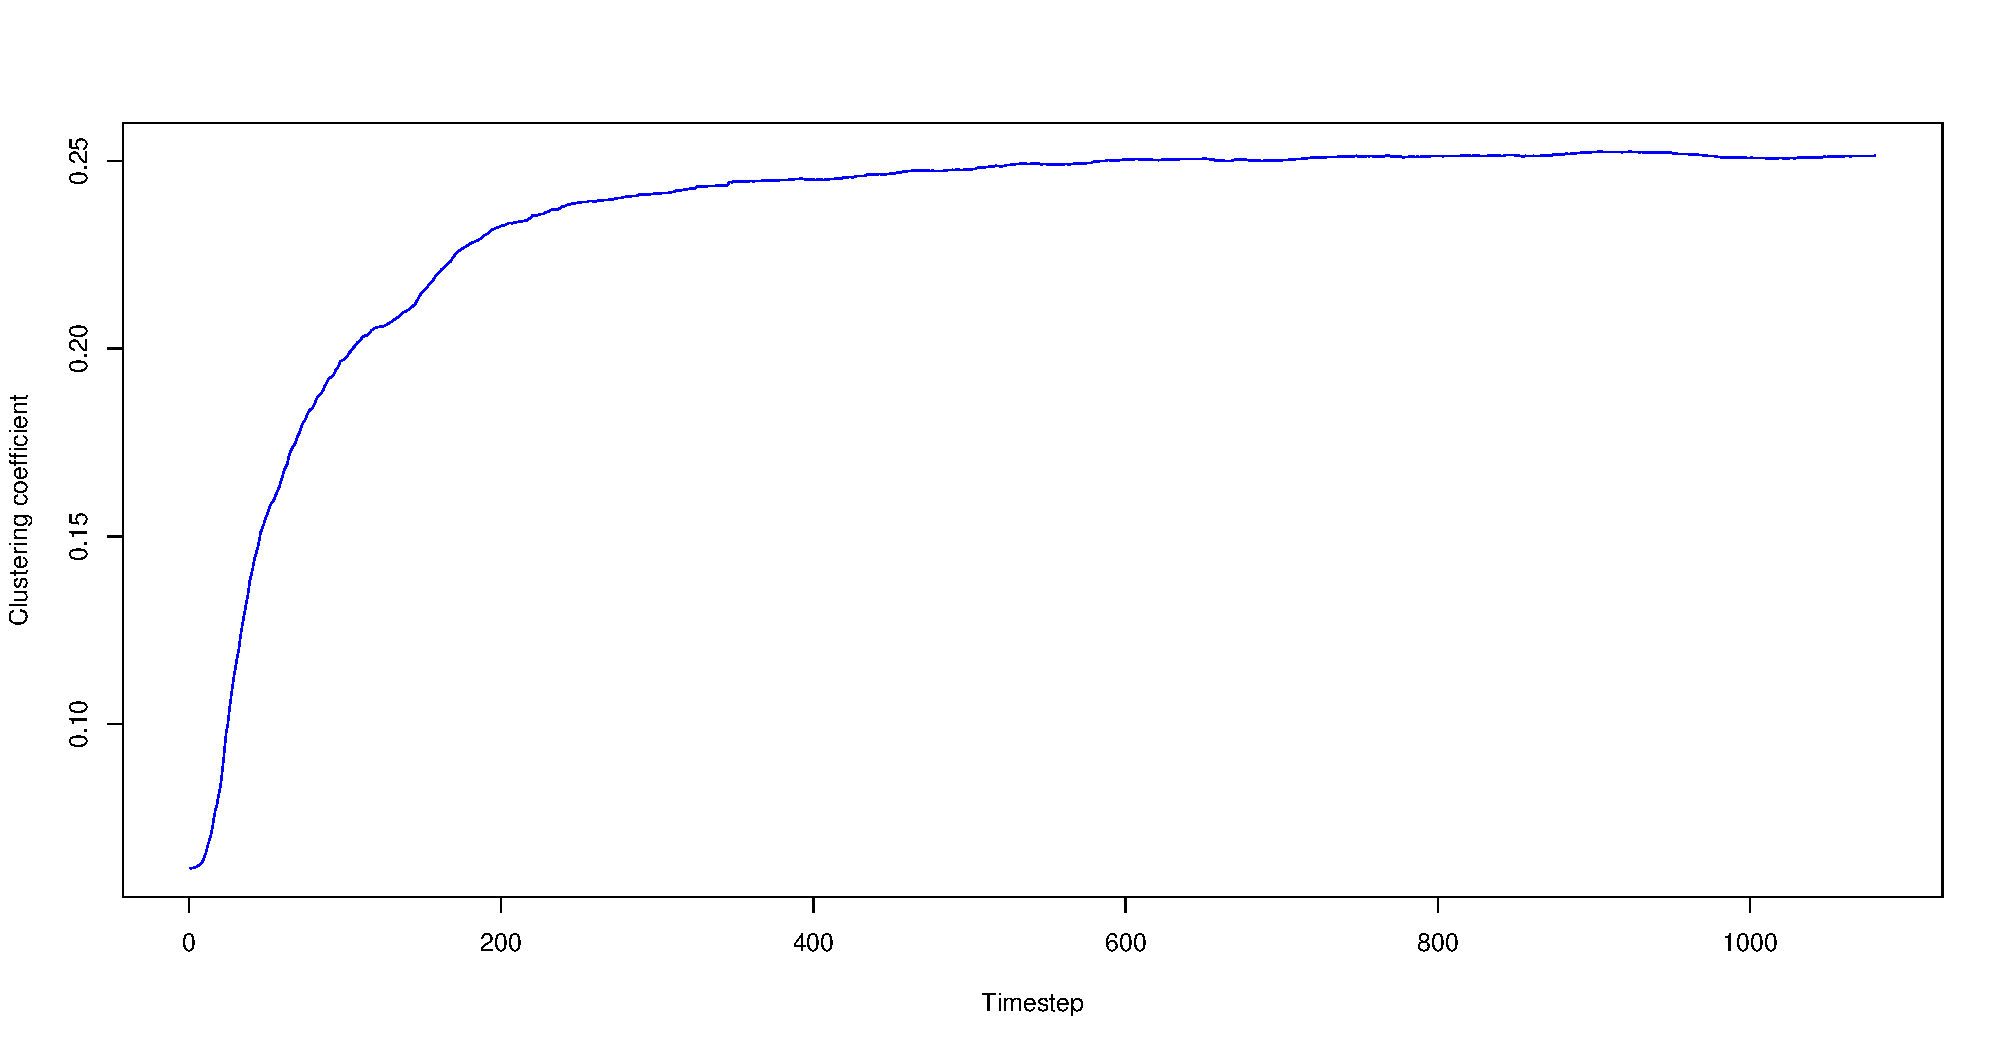
\includegraphics[width=81mm]{images/clustering_1000_rnd_1080_5_0.pdf} \\
a. Densità & b. Coefficiente di clustering \\[6pt]
 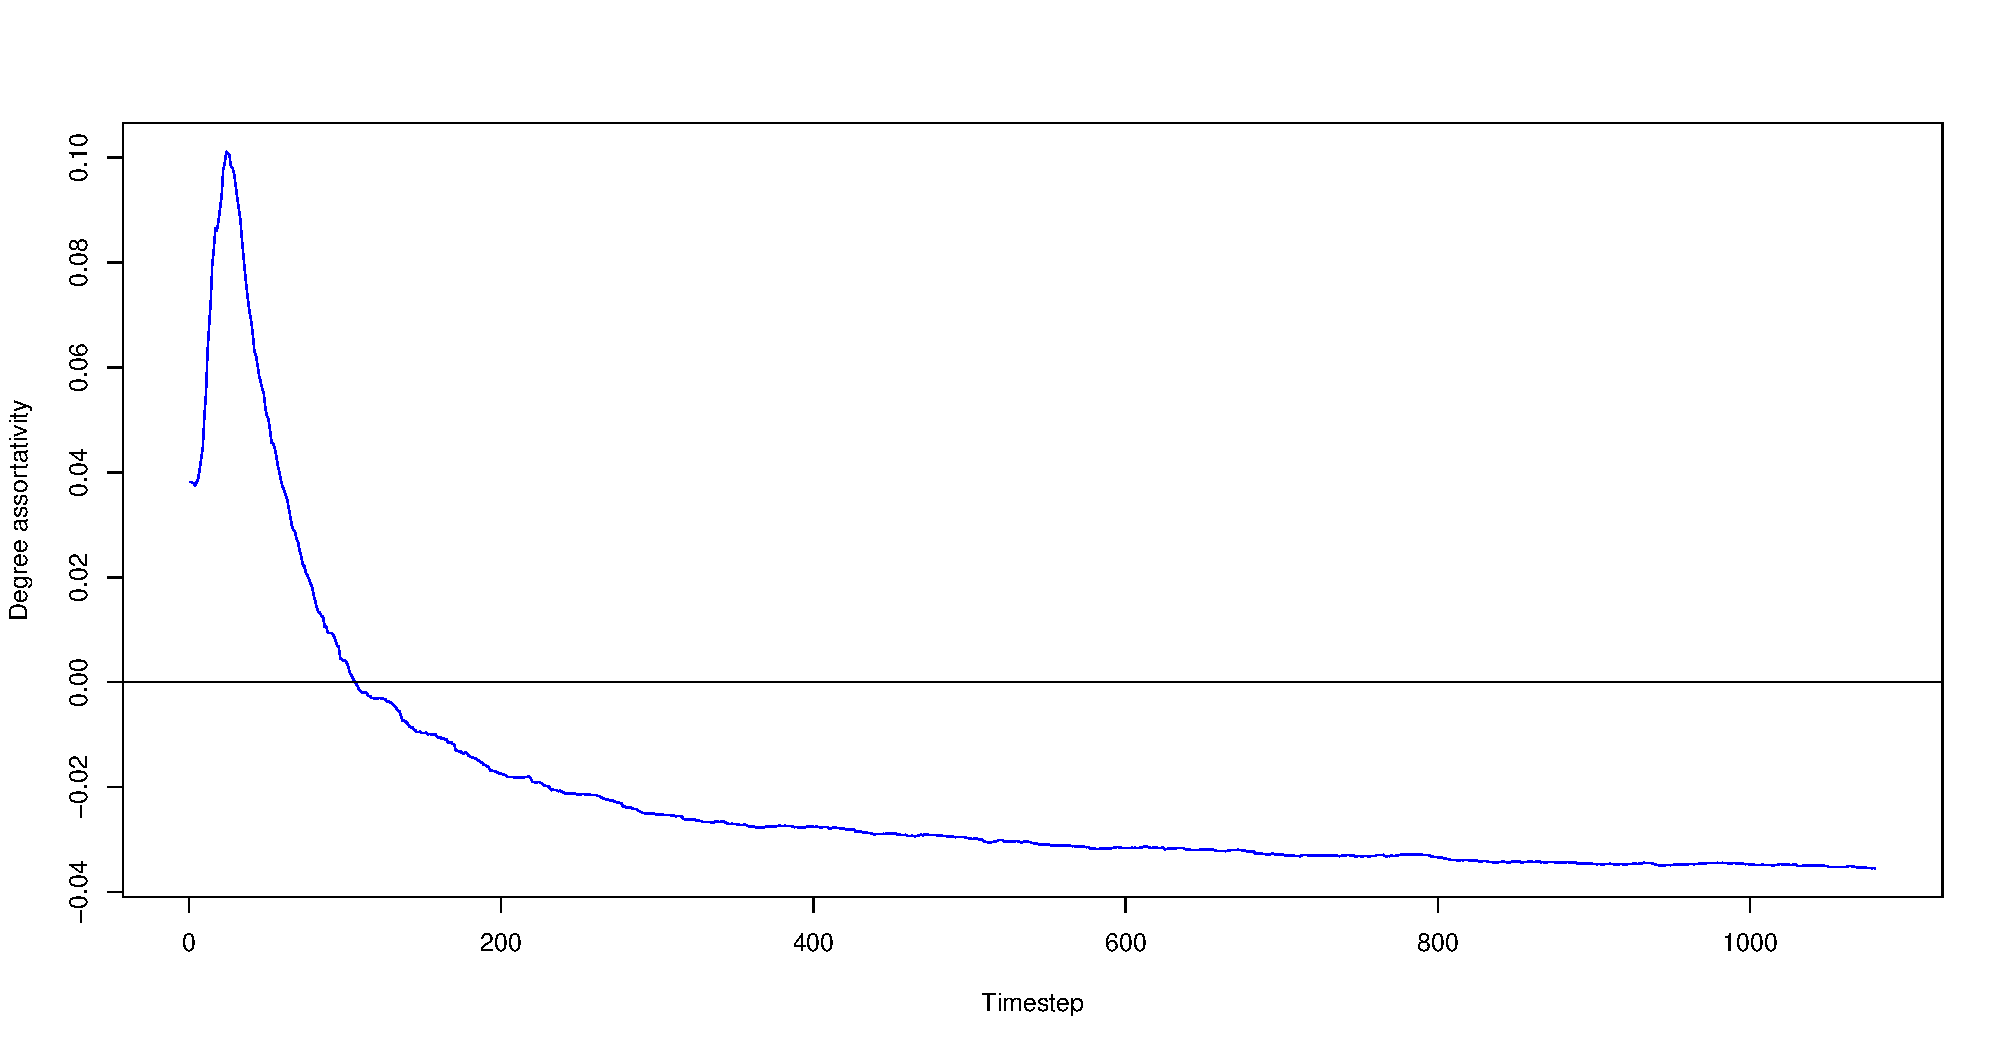
\includegraphics[width=81mm]{images/deg_assortativity_1000_rnd_1080_5_0.pdf} &   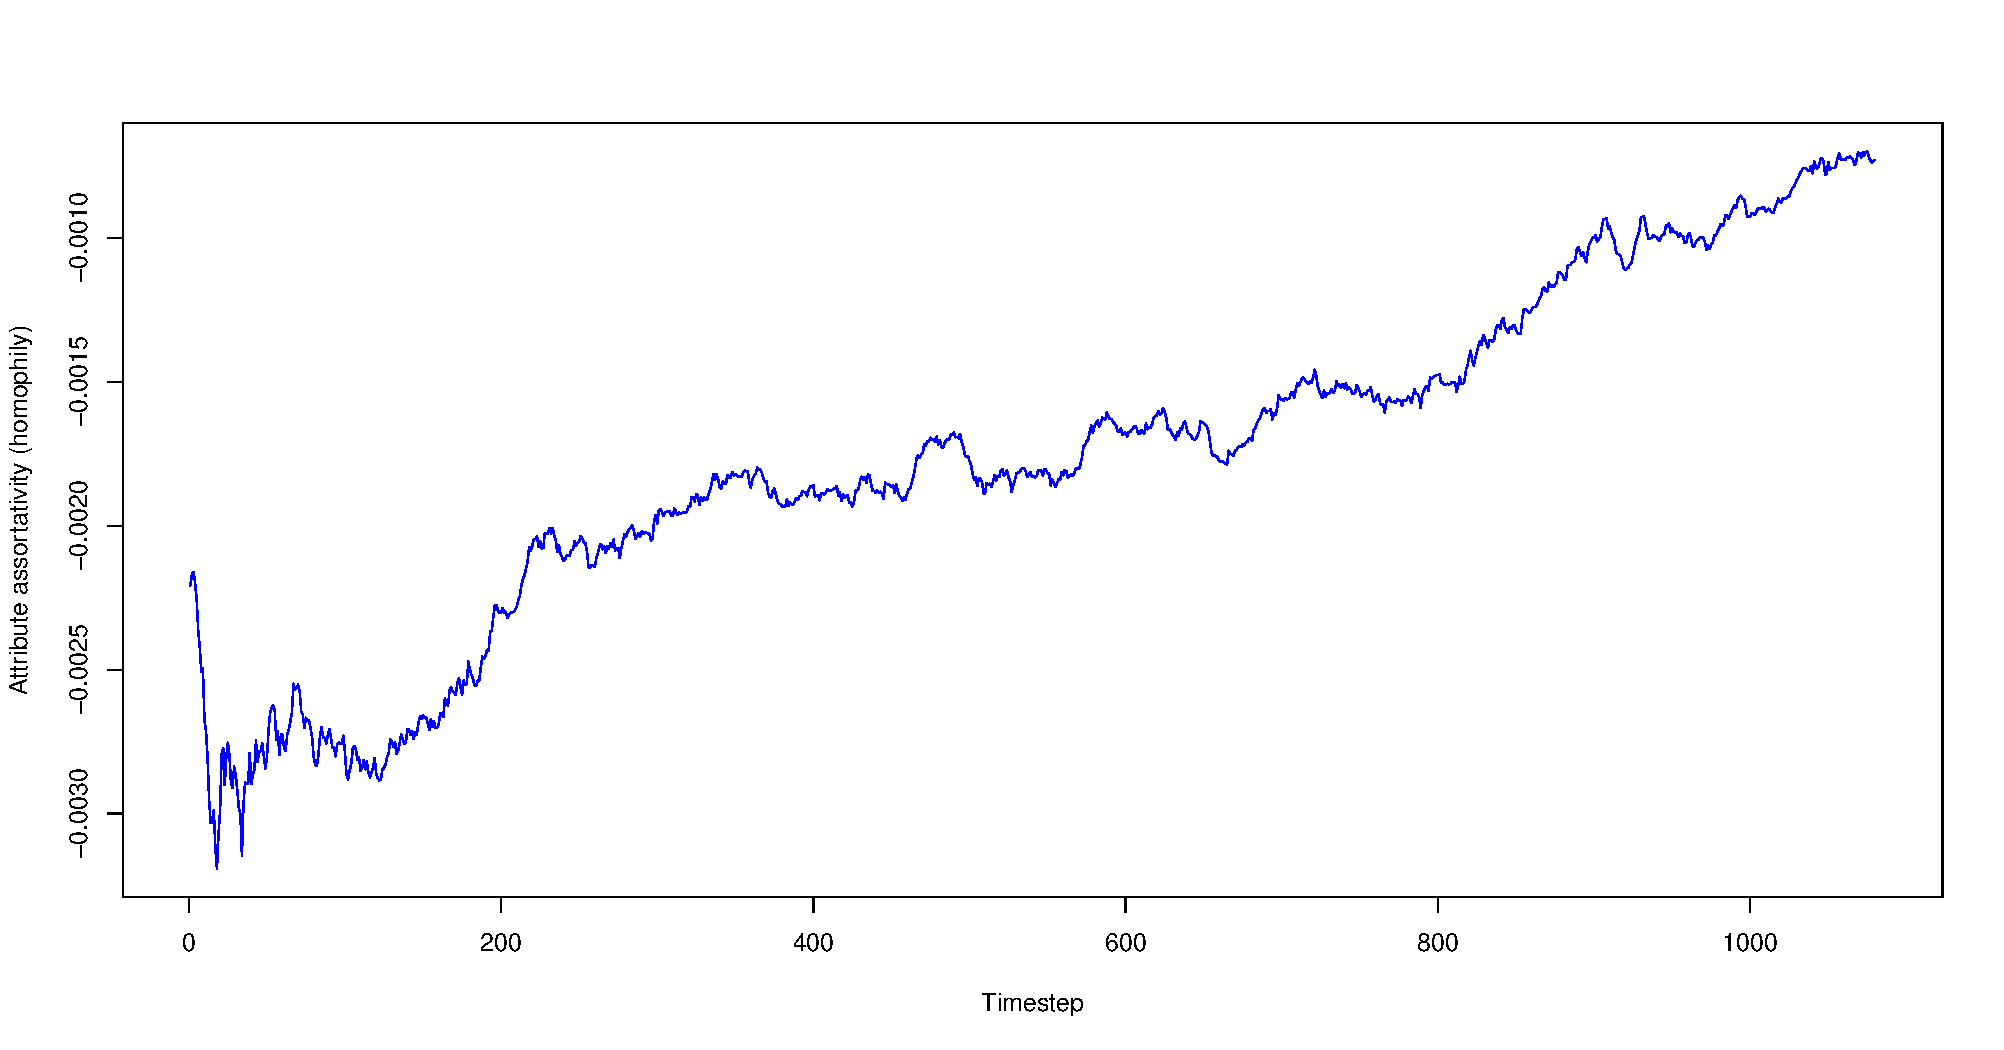
\includegraphics[width=81mm]{images/homophily_1000_rnd_1080_5_0.pdf} \\
c. Assortatività per grado & d. Assortatività per attributo \\[6pt]
\end{tabular}
\centering
\caption{Indici random network, densità 5.0\%}
\label{fig:rnd5}
\end{figure}
Le run con densità di partenza pari all'$1.0\%$ e al $5.0\%$ (figure \ref{fig:rnd1} e \ref{fig:rnd5}) hanno prodotto risultati piuttosto simili, e condividono un fenomeno importante: la densità, dopo un'iniziale fase di crescita, tende a rallentare la sua corsa con approssimazione logaritmica, attestandosi, nell'ultimo caso, poco sotto all'$8.0\%$. Sembra, quindi, che ci sia un limite alla crescita del numero di archi, per cui il completamento della rete (denstà $100\%$) sembra essere scongiurato. Il rallentamento viene percepito anche dal coefficiente di clustering, che decelera vistosamente fino a livellarsi. L'assortatività di scala presenta lo stesso fenomeno del primo e del terzo esperimento, ma lo sviluppo è più repentino man mano che si cresce con la densità iniziale: più collegamenti permettono ai nodi di avere più occasioni di instaurarne altri, per cui il processo di trasformazione da random network a rete ad invarianza di scala è più rapido. L'assortatività per attributo è poco indicativa, in quanto in un caso descresce e da positiva diventa negativa, per poi risalire in modo incerto, mentre nell'altro cresce costantemente ma resta negativa.

\begin{figure}[H]
\begin{tabular}{cc}
  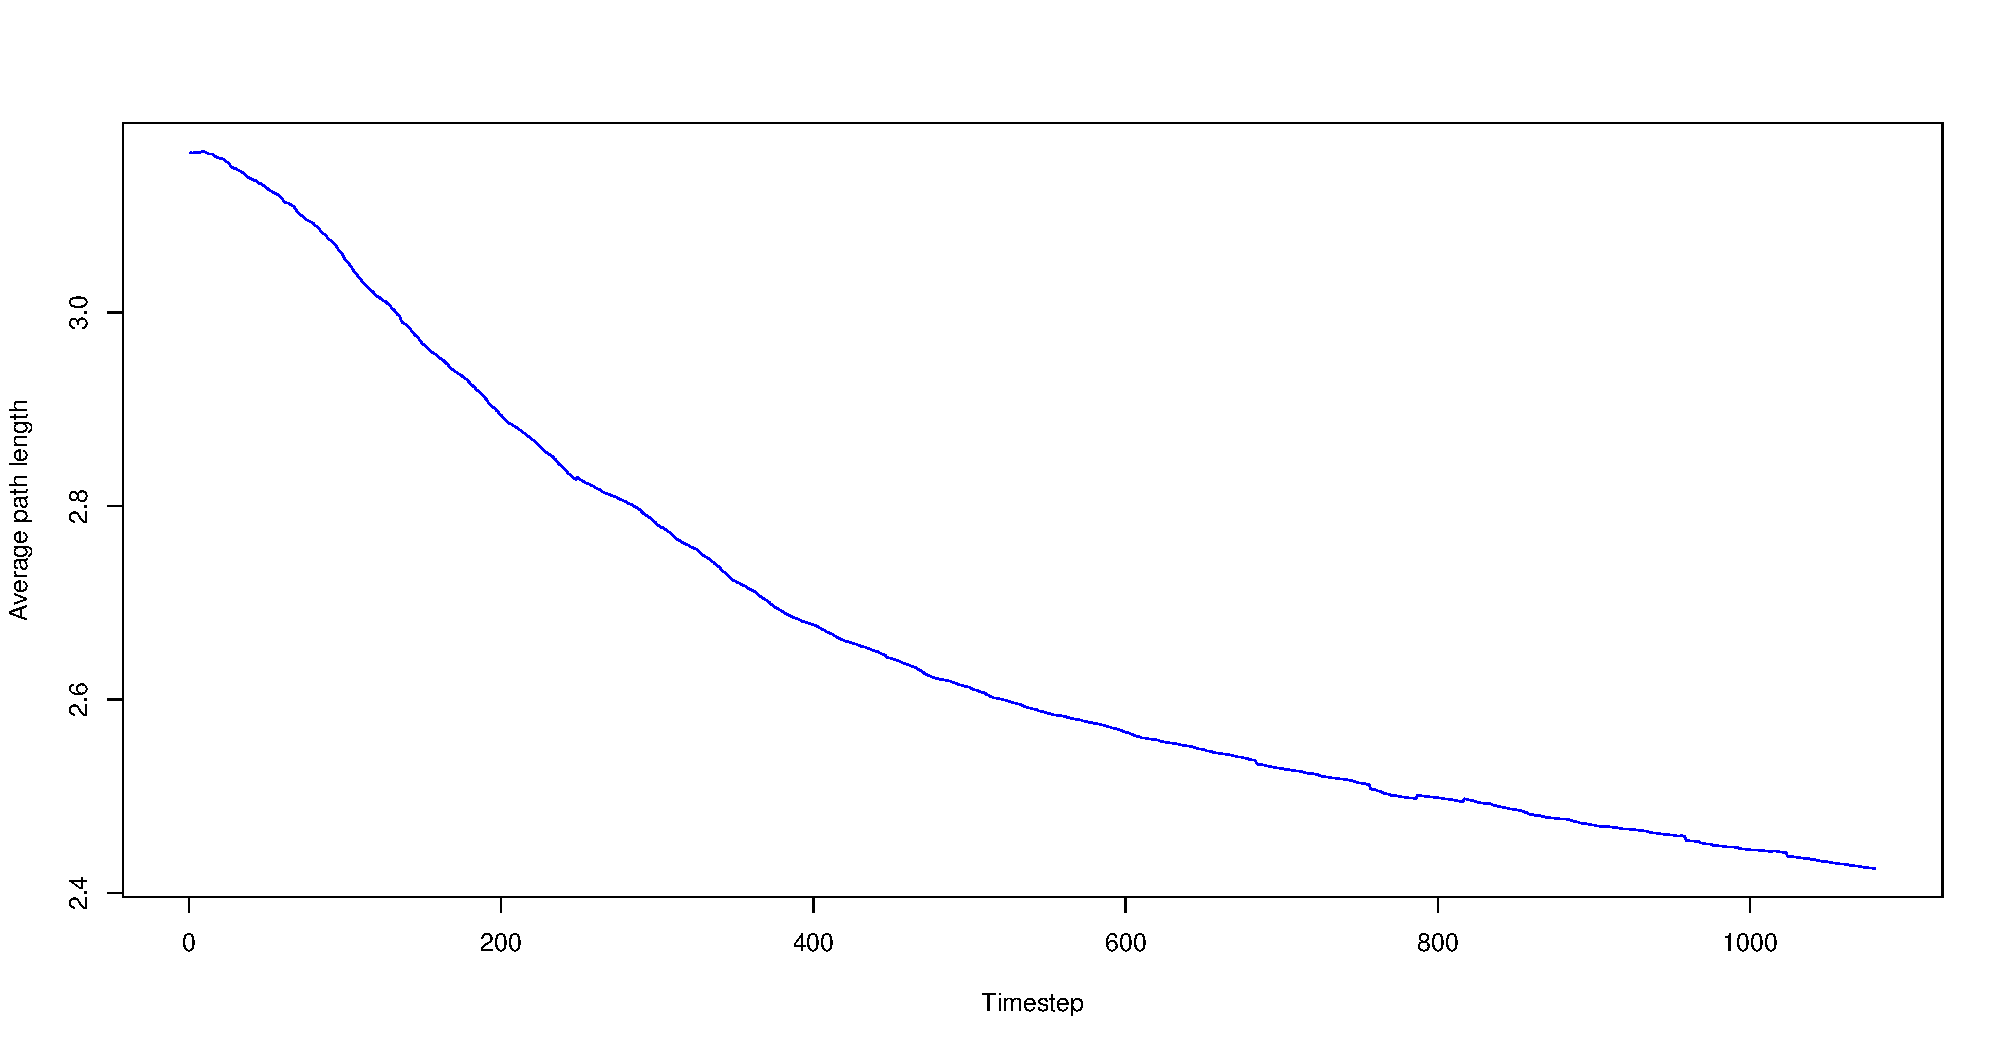
\includegraphics[width=81mm]{images/spath_1000_rnd_1080_1_0.pdf} &   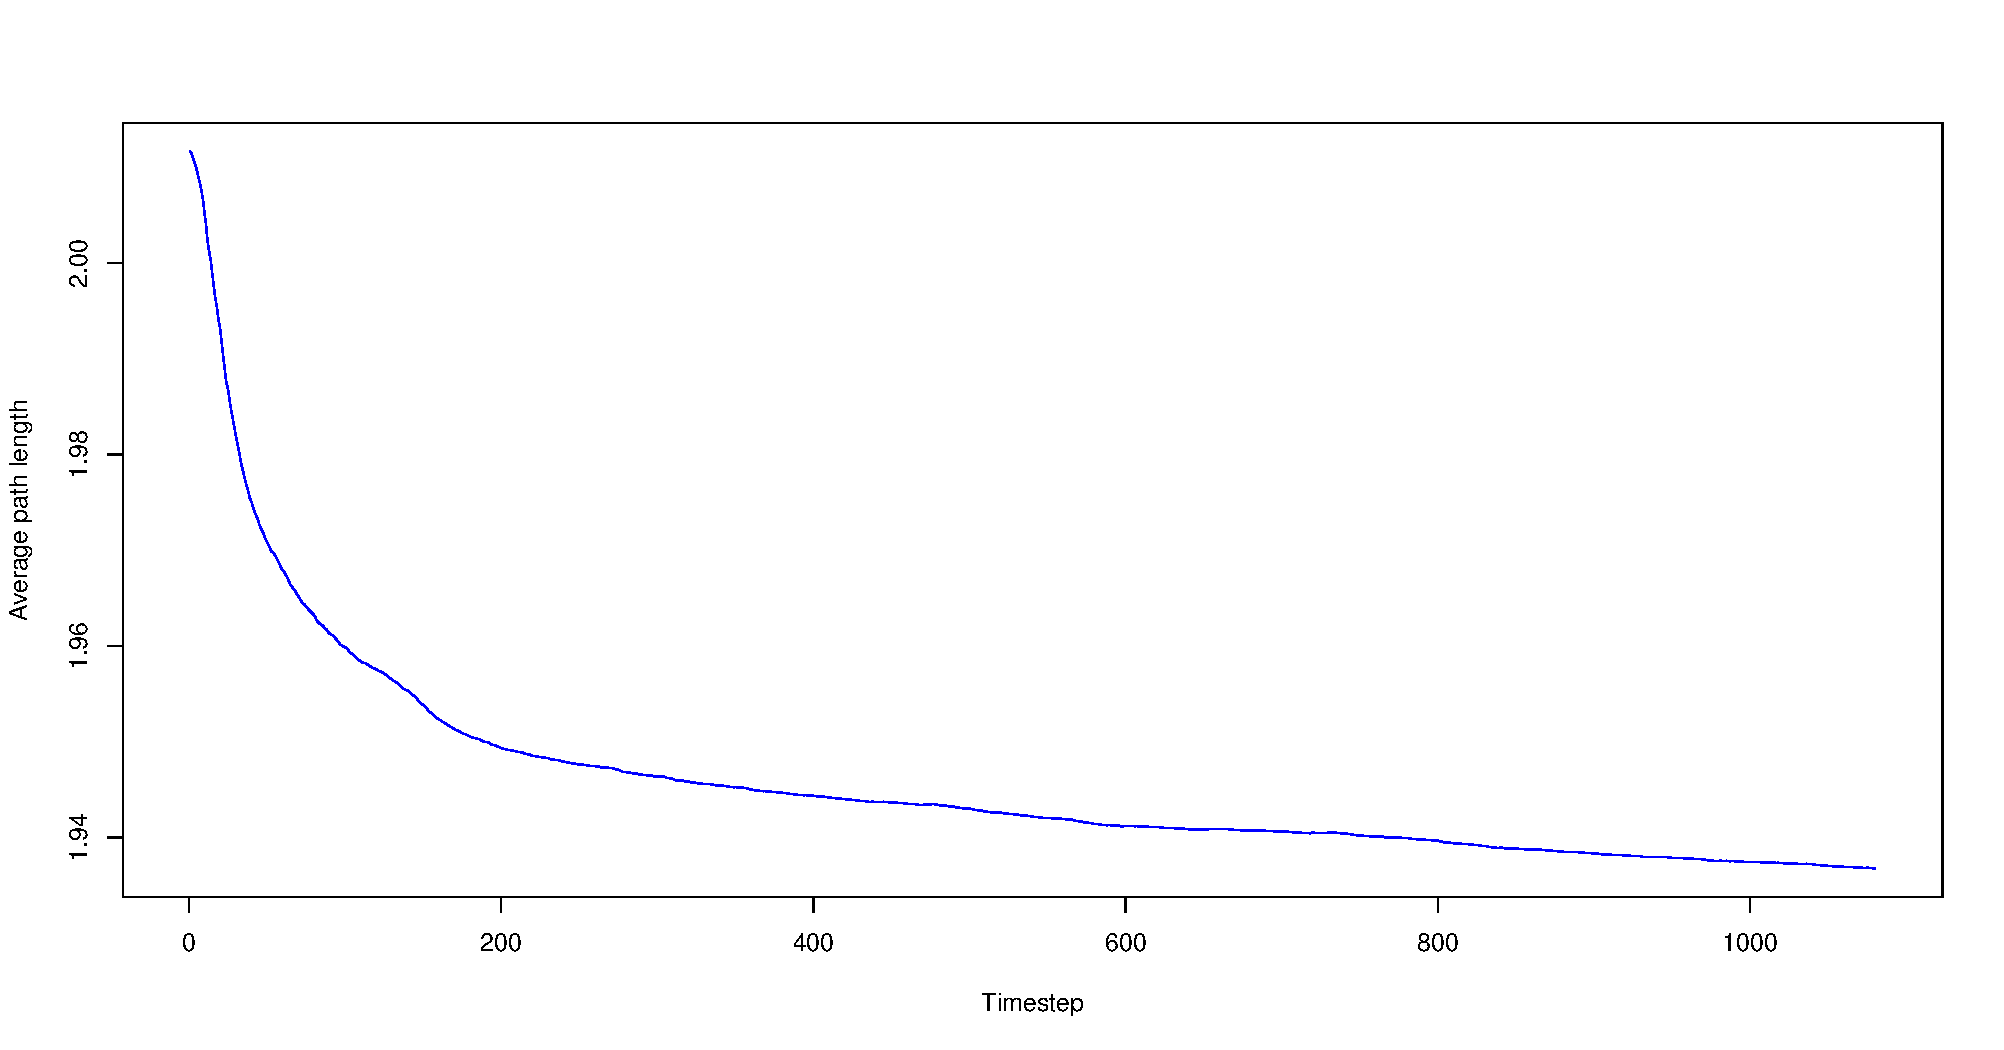
\includegraphics[width=81mm]{images/spath_1000_rnd_1080_5_0.pdf} \\
a. Densità 1.0\% & b. Densità 5.0\% \\[6pt]
\end{tabular}
\centering
\caption{Cammino minimo medio}
\label{fig:spath}
\end{figure}
Per questi ultimi due esperimenti è stato possibile calcolare fin dalla prima iterazione il \textit{cammino minimo medio} (figura \ref{fig:spath}). Com'era prevedibile, in entrambi i casi è sempre decrescente, per via della crecente densità; é interessante notare come nel caso con densità $5.0\%$ il cammino minimo medio scenda al di sotto della soglia dei due step. Esiste perciò un numero non indifferente di cammini composti solo da un arco, per cui ogni nodo ha accesso nel suo \textit{fov} una grande quantità di retweet provenienti da nodi inizialmente piuttosto lontani. Ci si aspetterebbe quindi che questo porti a una crescita esponenziale delle connessioni, in realtà le limitazioni poste nel modello riescono a limitarne l'esplosione. \\ \\
Richiamando quanto detto nella sezione \ref{subsec:graph}, una rete è detta ad invarianza di scala, o scale-free, se la distribuzione dei gradi (in-degree o out-degree) dei suoi nodi segue una power law. Le figure \ref{fig:sfd}, \ref{fig:rndd01}, \ref{fig:rndd05}, \ref{fig:rndd1} e \ref{fig:rndd5} mostrano il plot della distribuzione iniziale (verde) e della distribuzione finale (rossa), dell'\textit{in-degree} dei nodi in ogni esperimento di questa sezione, normalizzati per il numero massimo di in-degree in modo da poterne confrontare l'andamento. \'E importante notare che la curva verde della figura  è stata generata secondo una power law, quindi rappresenta un modello di rete ad invarianza di scala ``ideale"; normalizzata in questa maniera, può quindi essere presa come modello di riferimento anche per gli altri esperimenti, perciò l'abbiamo riportata (in blu) in tutti gli altri grafici. \\ \\
La prima esecuzione del modello (figura \ref{fig:sfd}) non va a modificare sostanzialmente la natura scale free della rete, in quanto la distribuzione in uscita è solo leggermente deformata. Nella seconda run (figura \ref{fig:rndd01}) è lampante come la costruzione random iniziale sia distante dal modello a invarianza di scala, e, nonostante l'esecuzione del nostro modello, la distribuzione dell'in-degree non cambia. Nella terza run (figura \ref{fig:rndd05}) si ha una situazione di partenza analoga alla precedente, con la sola differenza della densità; dopo l'esecuzione del modello però, la curva è molto più simile ad una power law rispetto al caso precedente. Il nostro modello sembra quindi adattare, con un aiuto derivante dalla relativamente elevata densità, una random network ad una rete scale-free. Questo fenomeno viene ulteriormente accentuato dal caso con densità di partenza all'$1.0\%$ (figura \ref{fig:rndd1}): nonostante una curva di partenza di tipo randomico, la curva finale si discosta di poco da quella ideale. Un discorso a sè stante spetta per l'ultima run (figura \ref{fig:rndd5}), dove la rete randomica istanziata in partenza presenta già una distribuzione dell'in-degree molto simile ad una power law, e l'esecuzione del nostro modello non fa altro che accentuare la distanza tra i nodi ``popolari" e quelli meno importanti.
\begin{figure}[H]
\centering
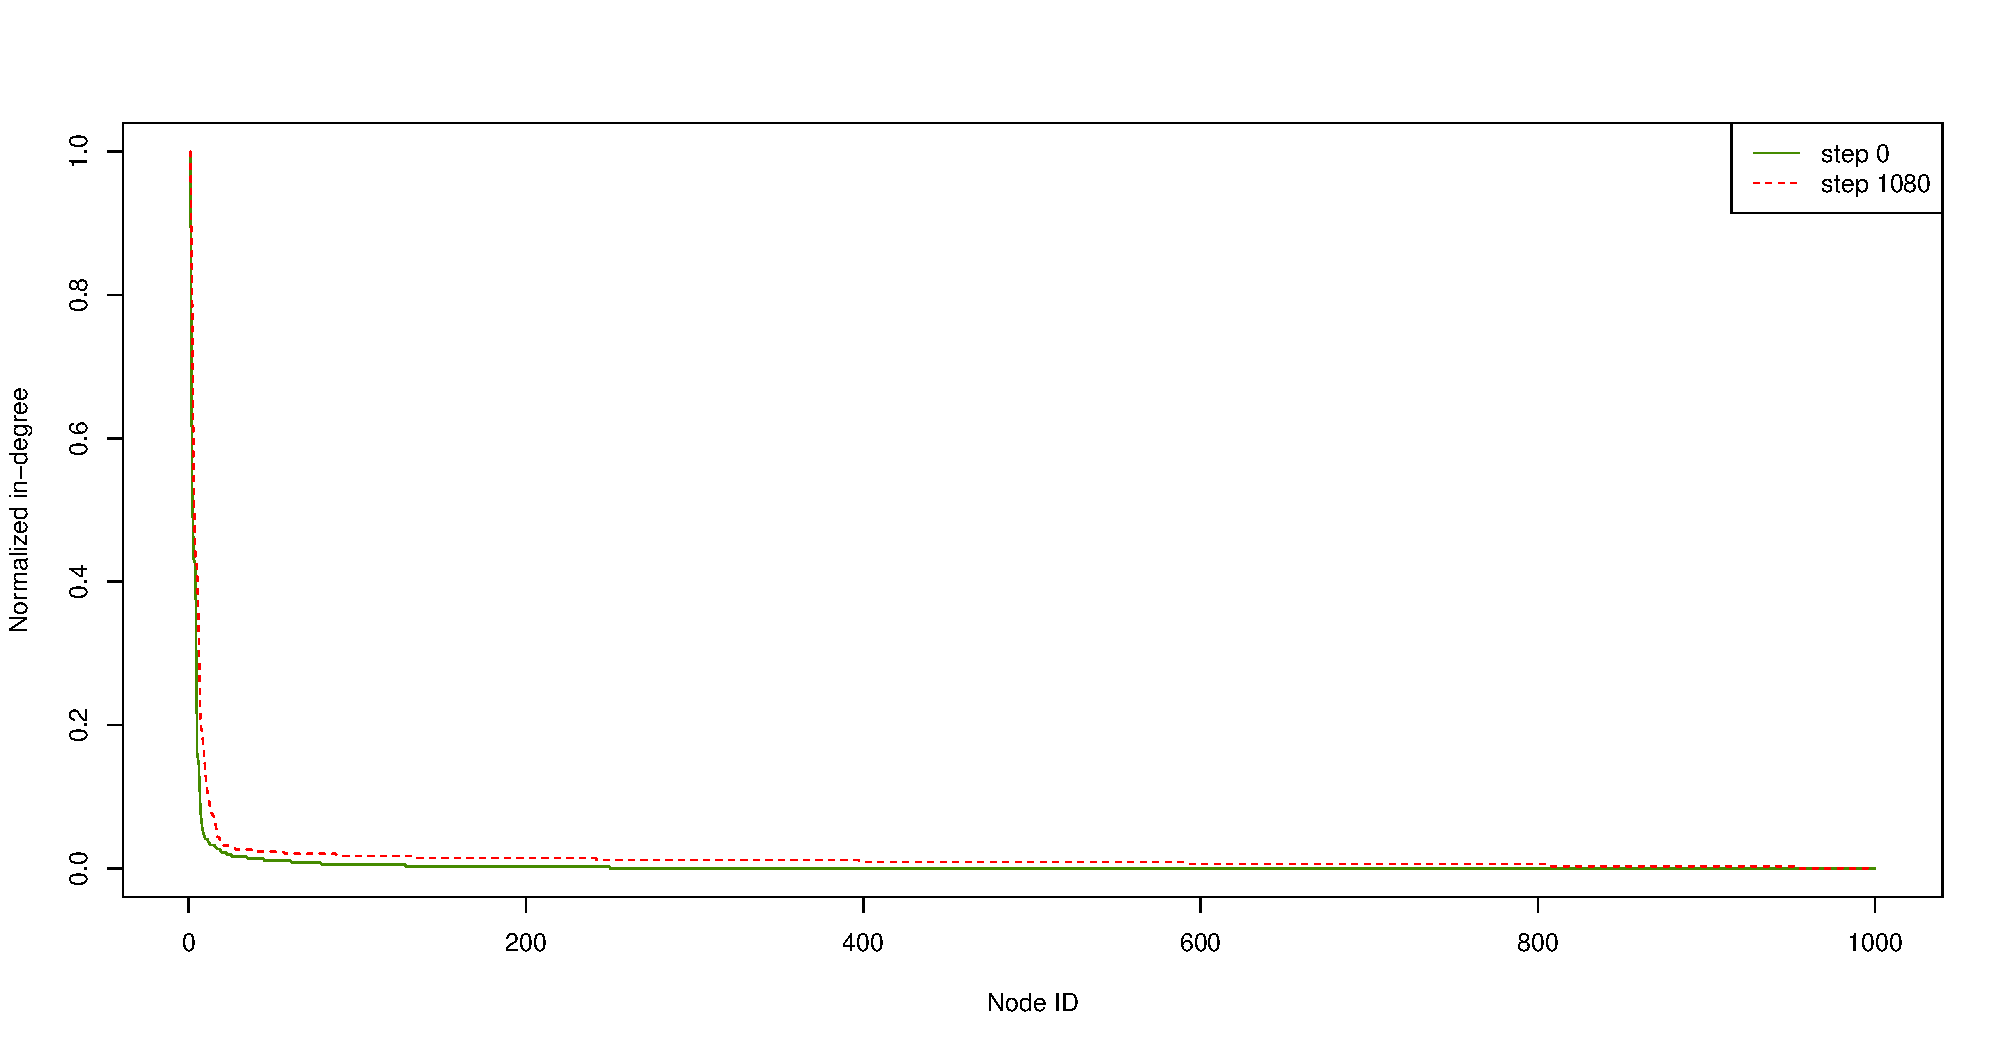
\includegraphics[scale=0.5]{images/dist_1000_sf_1080_0.pdf}
\caption{Distribuzione in-degree della rete scale-free, densità 0.1\%}
\label{fig:sfd}
\end{figure}
\begin{figure}[H]
\centering
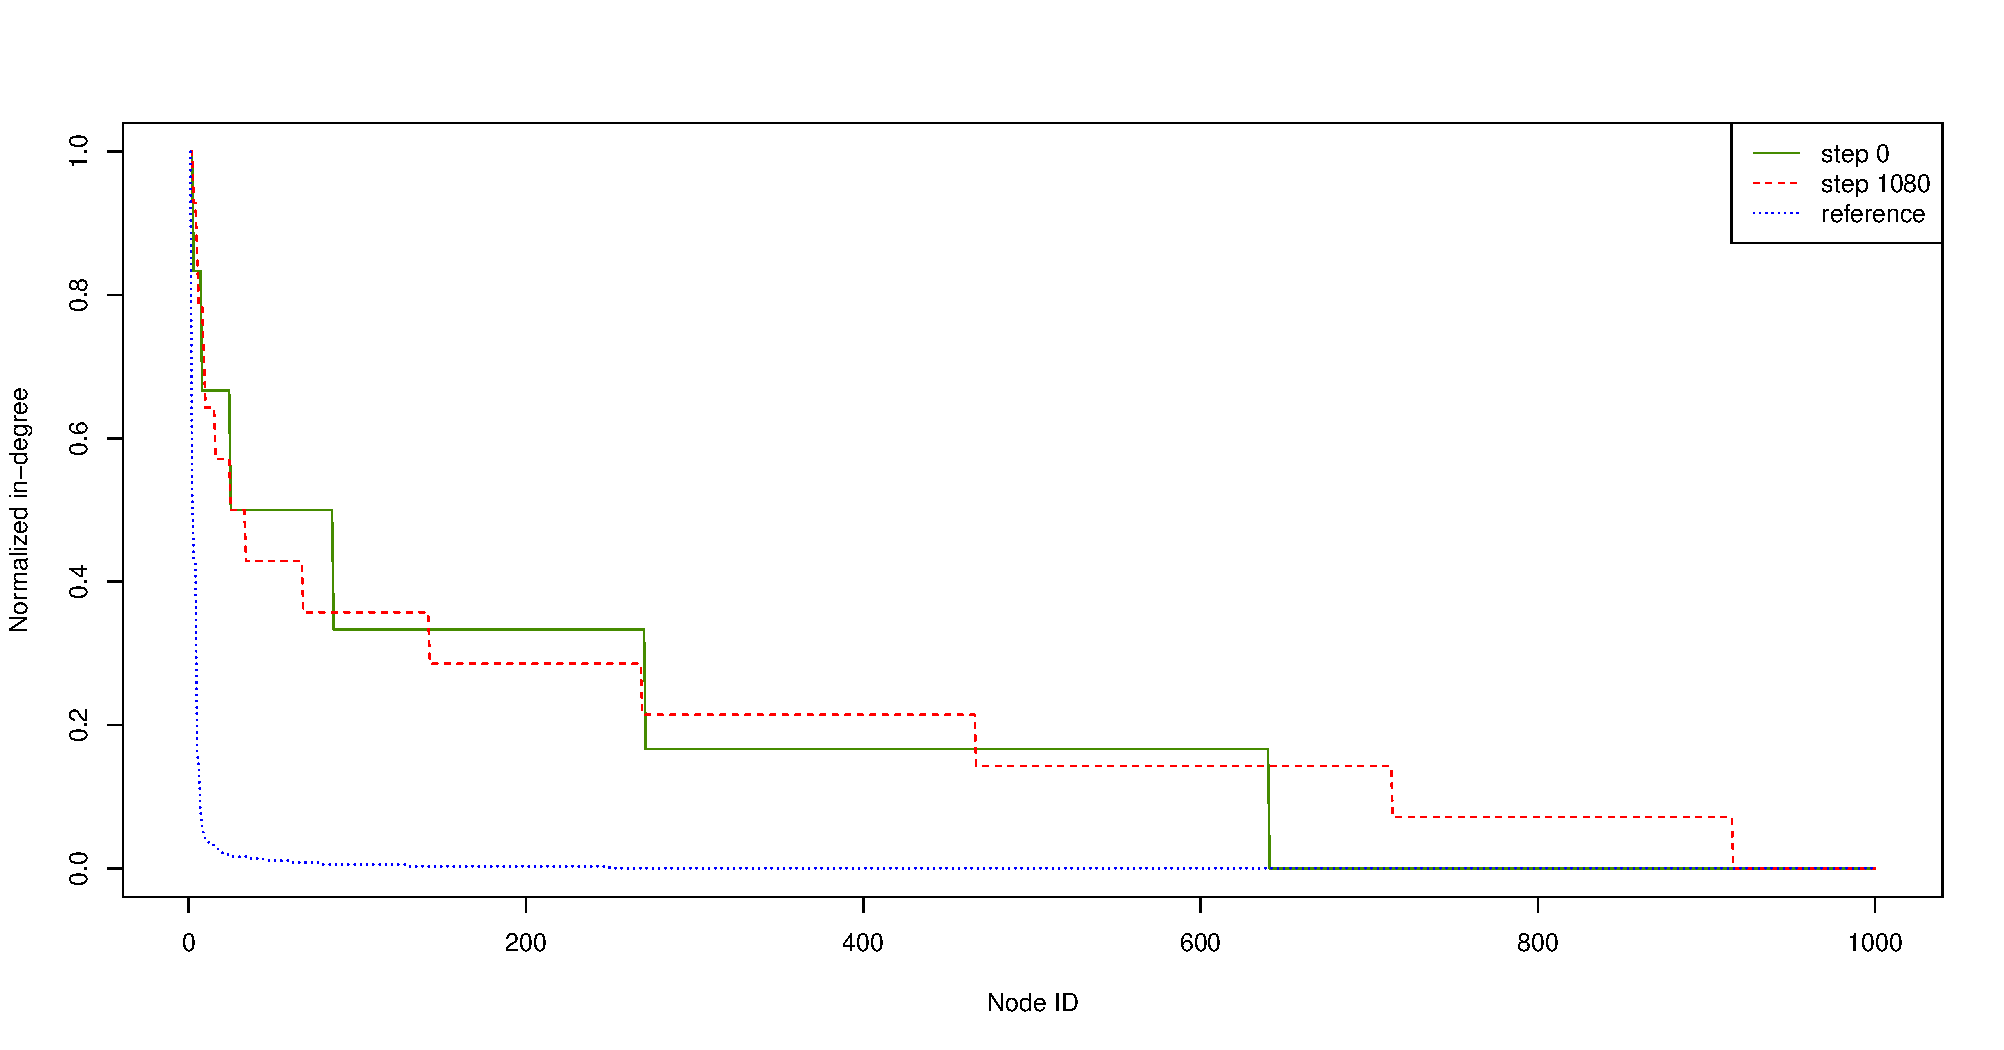
\includegraphics[scale=0.5]{images/dist_1000_rnd_1080_01_0.pdf}
\caption{Distribuzione in-degree della rete random, densità 0.1\%}
\label{fig:rndd01}
\end{figure}
\begin{figure}[H]
\centering
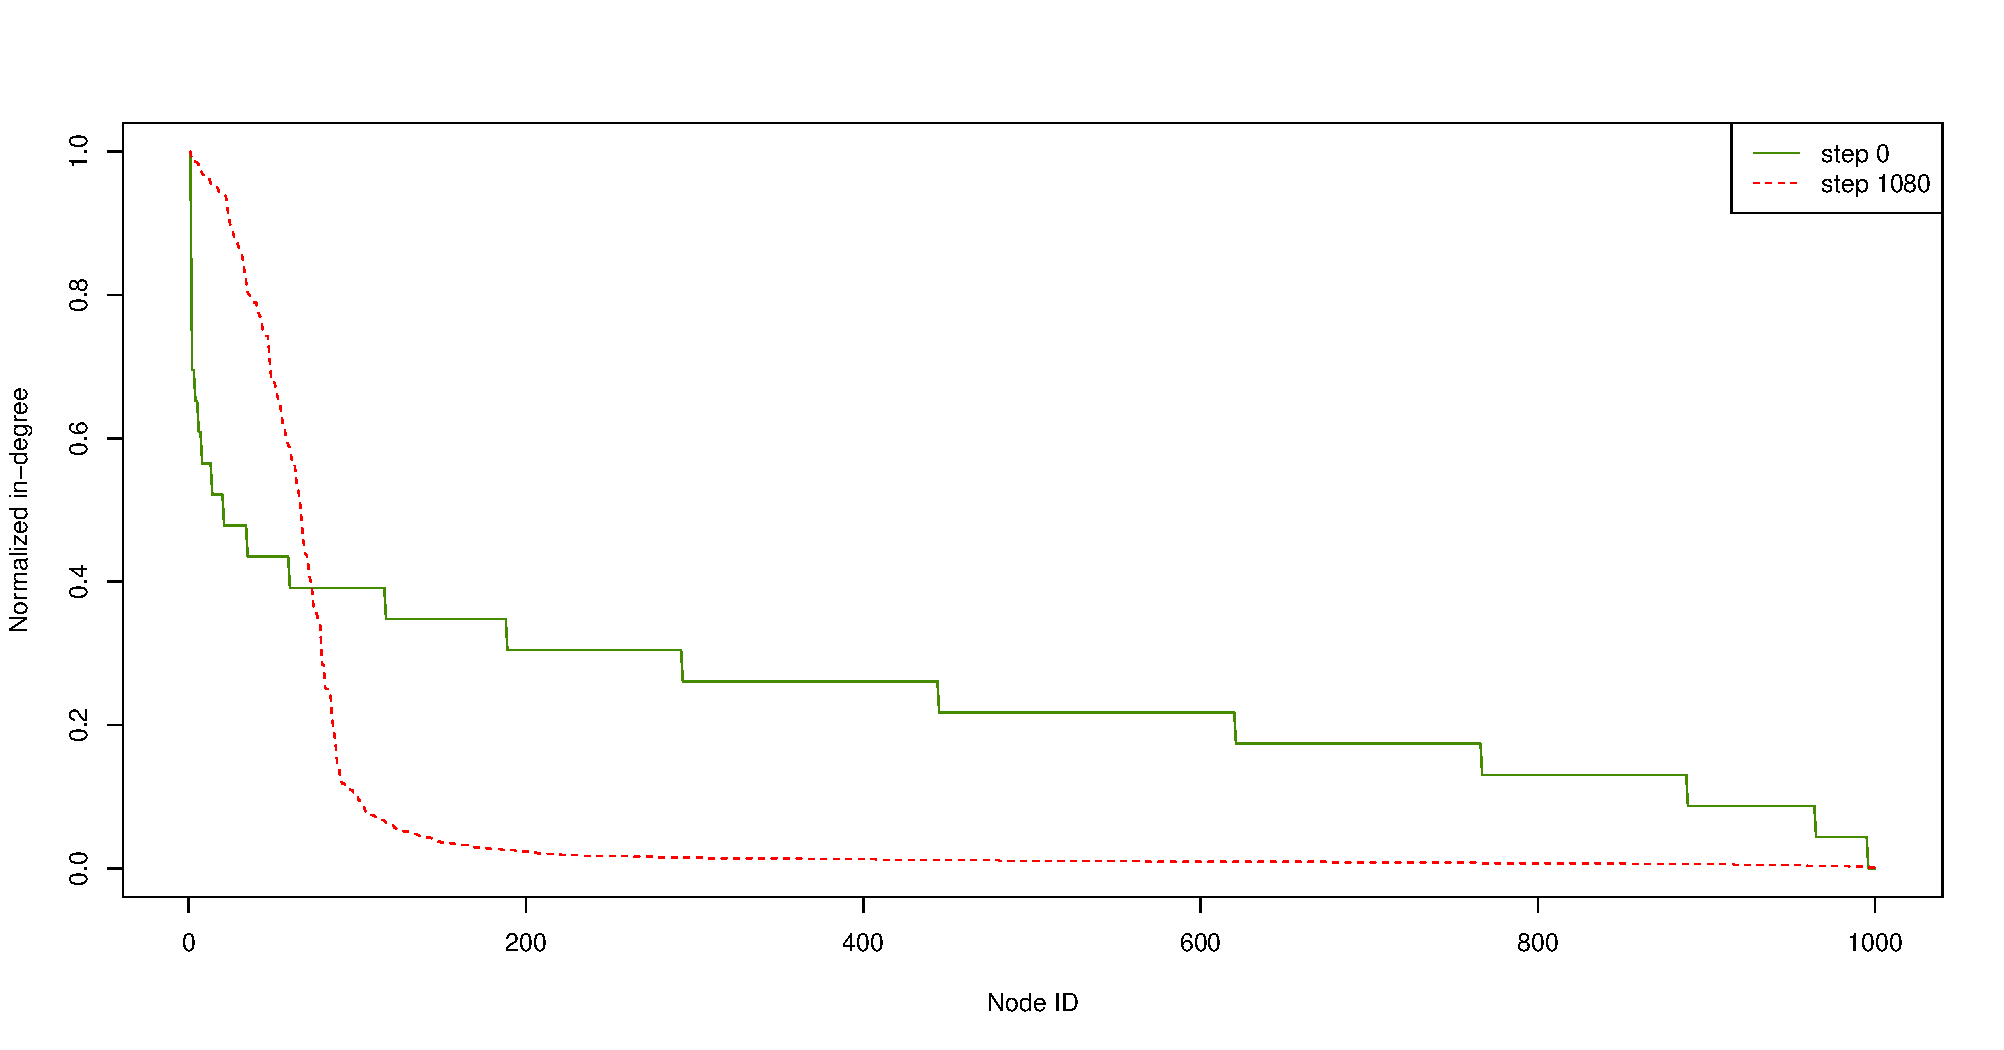
\includegraphics[scale=0.5]{images/dist_1000_rnd_1080_05_0.pdf}
\caption{Distribuzione in-degree della rete random, densità 0.5\%}
\label{fig:rndd05}
\end{figure}
\begin{figure}[h]
\centering
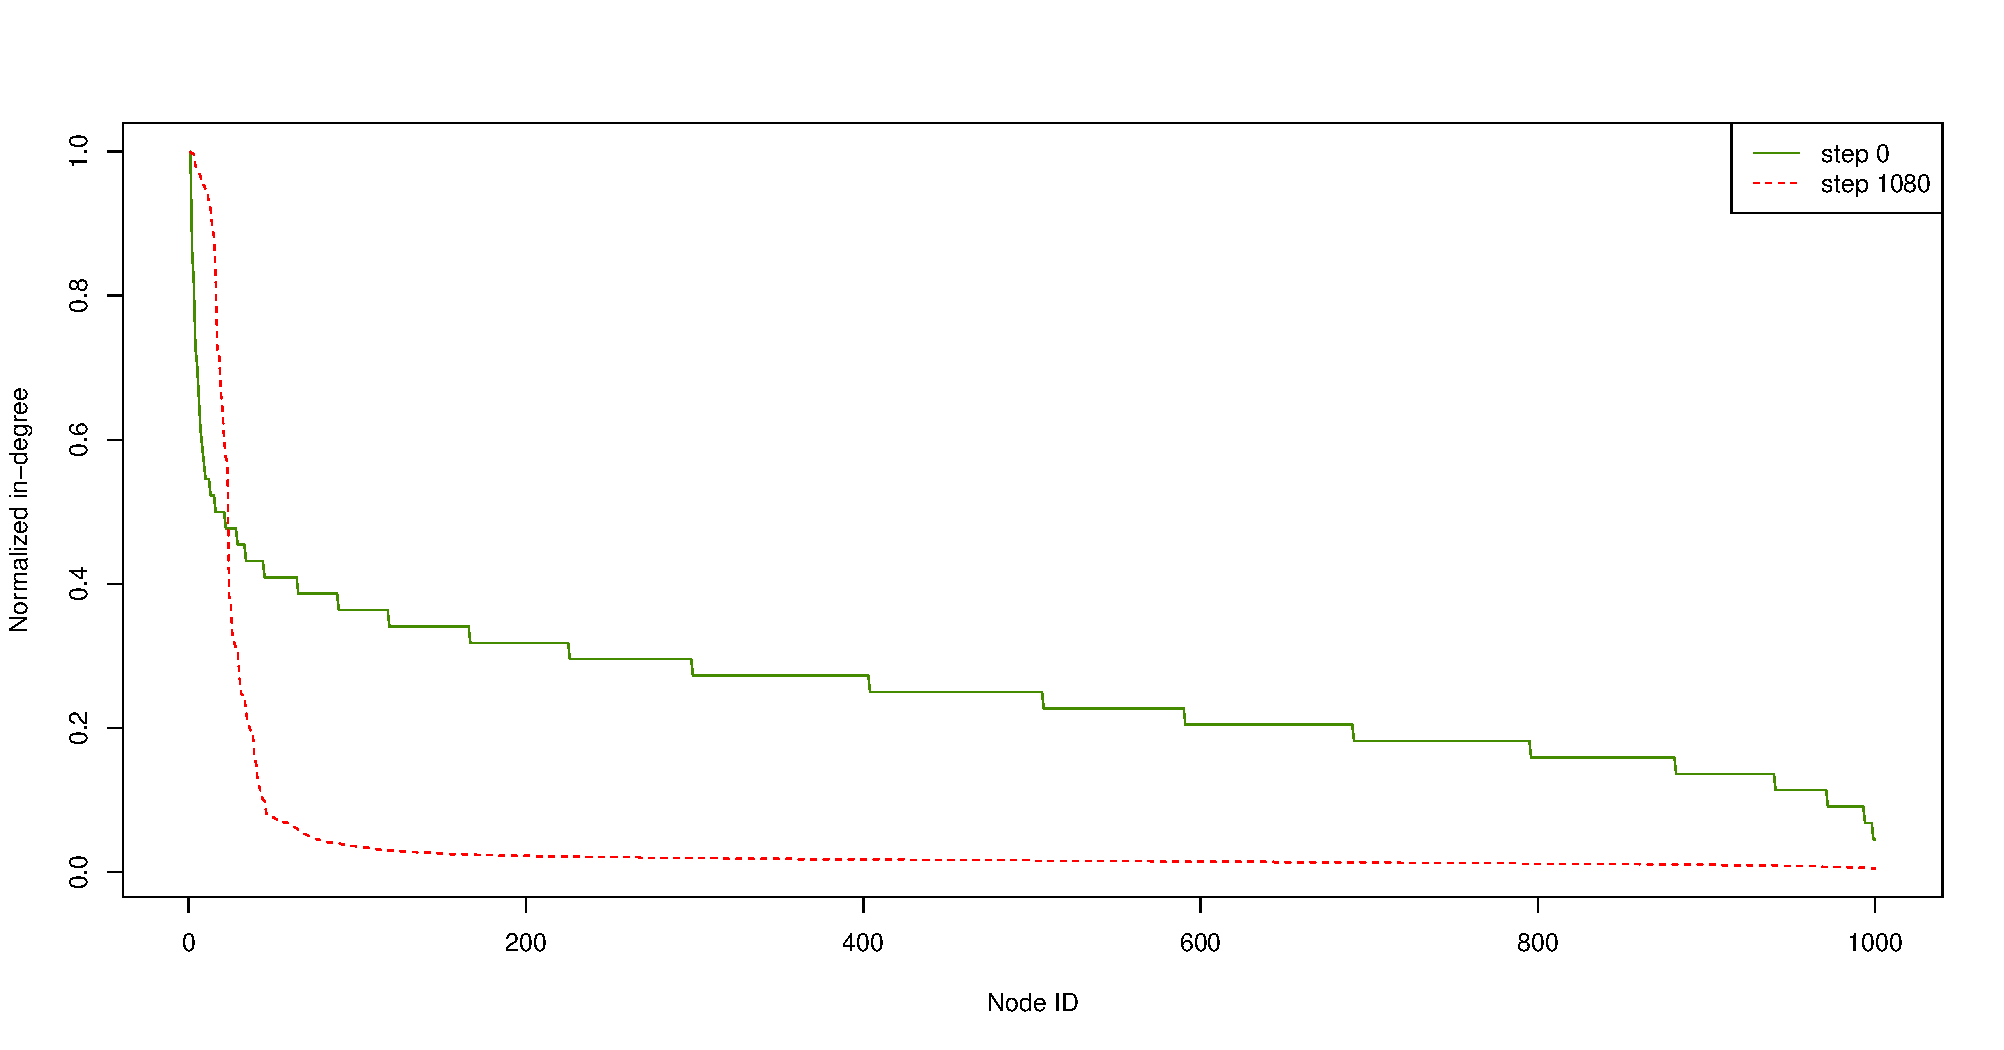
\includegraphics[scale=0.5]{images/dist_1000_rnd_1080_1_0.pdf}
\caption{Distribuzione in-degree della rete random, densità 1.0\%}
\label{fig:rndd1}
\end{figure}
Sembra quindi che ci sia una certa correlazione tra l'indice di assortatività per grado visto in precedenza e l'andamento delle distribuzioni dell'in-degree, in quanto i casi che presentavano un comportamento ``a cuspide" nella misura di assortatività tendono a rispettare il comportamento di una rete ad invarianza di scala, in particolare la run con rete scale-free e le run con rete random con valori di densità $0.5\%$, $1.0\%$ e $5.0\%$. 
\begin{figure}[H]
\centering
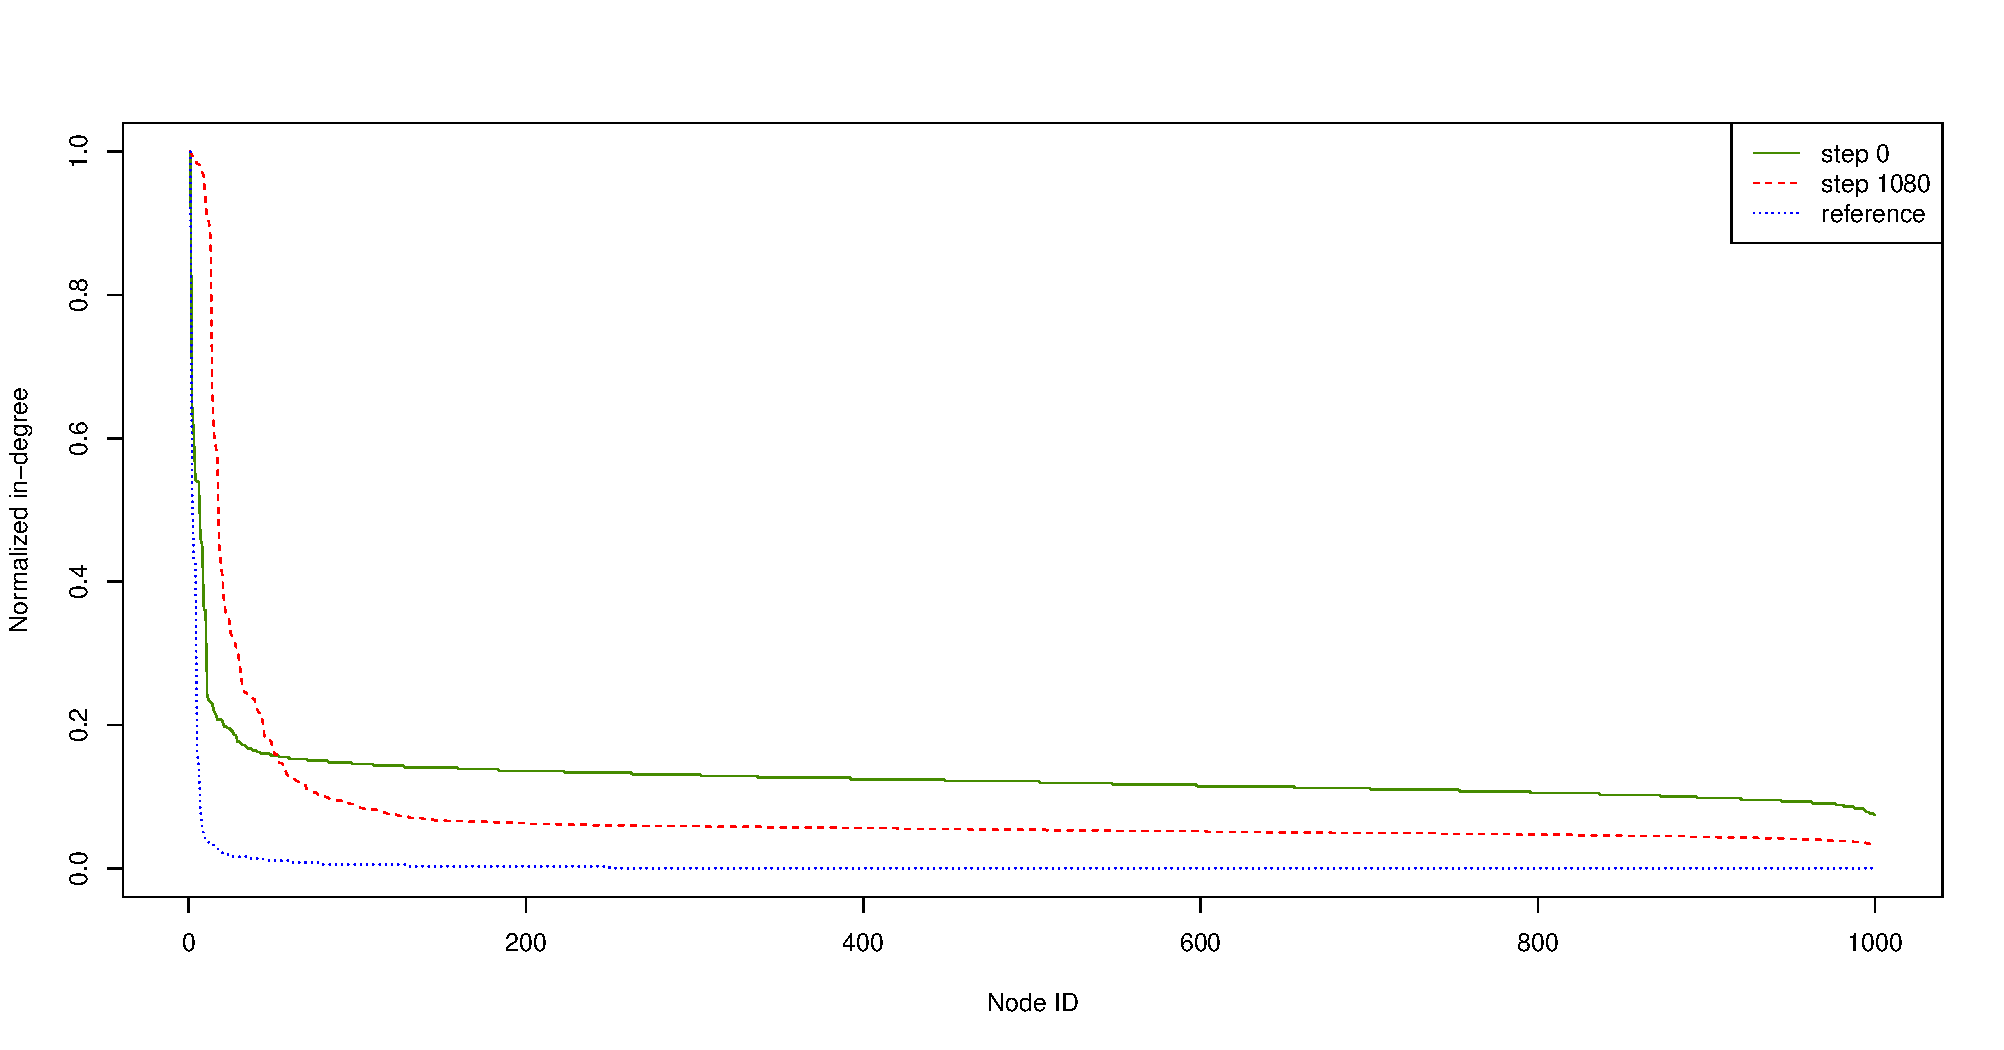
\includegraphics[scale=0.5]{images/dist_1000_rnd_1080_5_0.pdf}
\caption{Distribuzione in-degree della rete random, densità 5.0\%}
\label{fig:rndd5}
\end{figure}
Nella sezione \ref{subsec:graph} abbiamo esposto la definizione di invarianza di scala e di power law. Dai dati prodotti dagli esperimenti è possibile stimare i valori $C$ e $\gamma$ delle curve finali (in rosso) rappresentate nei plot precedenti. Nella libreria \textit{scipy} di Python è presente un'implementazione del \textit{metodo non lineare dei minimi quadrat}i: l'abbiamo utilizzata per stimare i parametri delle curve.
Nella tabella sottostante riportiamo i valori dei coefficienti $C$ e $\gamma$ della power law per le distribuzioni finali (in rosso) di tutte le run effettuate \textit{con instanziazione randomica della rete} 
\begin{center}
    \begin{tabular}{| l | l | l | l | l |}
    \hline
    Densità & 0.1\% & 0.5\% & 1.0\% & 5.0\% \\ \hline \hline
	$C$ & 22.11 & 1981.45 & 1832.28 & 1722.57 \\ \hline
	$\gamma$ & 0.36 & 0.55 & 0.63 & 0.55 \\ \hline
    \end{tabular}
\end{center}
In quest'altra tabella riportiamo i valori per le distribuzioni iniziale e finale della run effettuata \textit{con instanziazione scale-free della rete}:
\begin{center}
    \begin{tabular}{| l | l | l |}
    \hline
    Step & 0 & 1080 \\ \hline \hline
	$C$ & 386.26 & 390.65 \\ \hline
	$\gamma$ & 1.09 & 0.87 \\ \hline
    \end{tabular}
\end{center}
Da notare che la prima colonna di questa tabella contiente i parametri della curva di riferimento. \\
Per quanto riguarda le reti random, quella che alla fine delle iterazioni rispetta più fedelmente l'invarianza di scala è quella con densità di partenza posta all'$1.0\%$ (figura \ref{fig:grnd}). La migliore in assoluto è invece la run con la rete scale-free iniziale (figura \ref{fig:gsf}). Dai plot salta immediatamente all'occhio la differenza di densità tra le due soluzioni, e il diverso numero di nodi ``hub".
\begin{figure}[H]
\centering
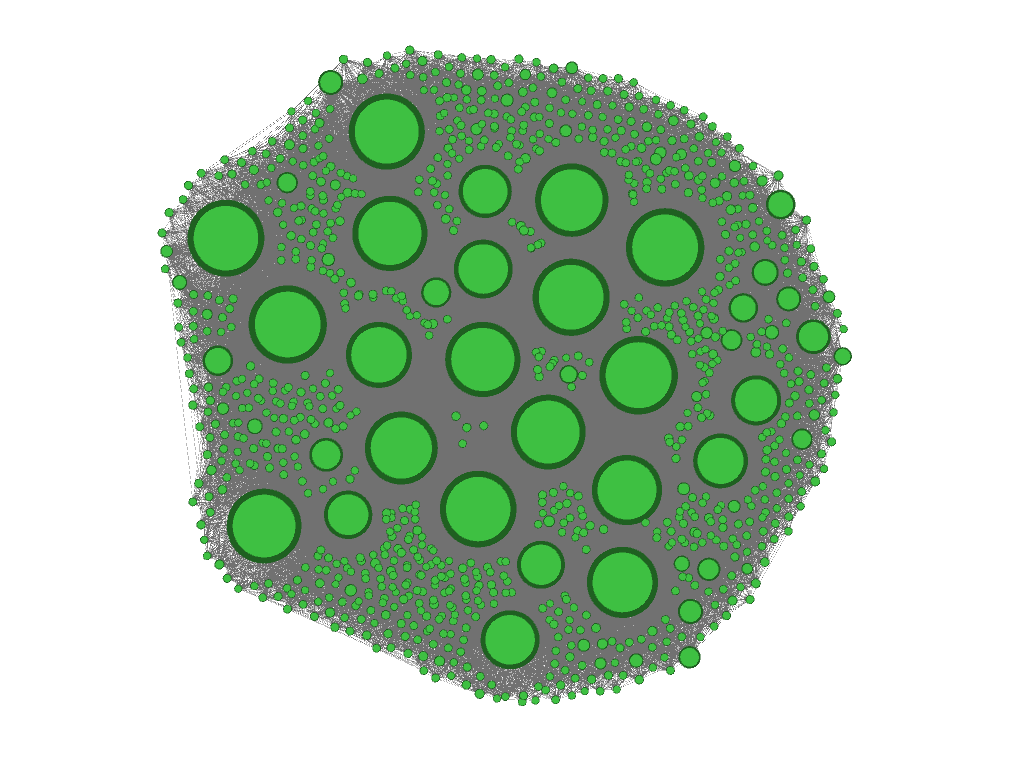
\includegraphics[scale=0.4]{images/init_1000_rnd_1080_1_0.png}
\caption{Grafo rete random, densità 1.0\%}
\label{fig:grnd}
\end{figure}
\begin{figure}[H]
\centering
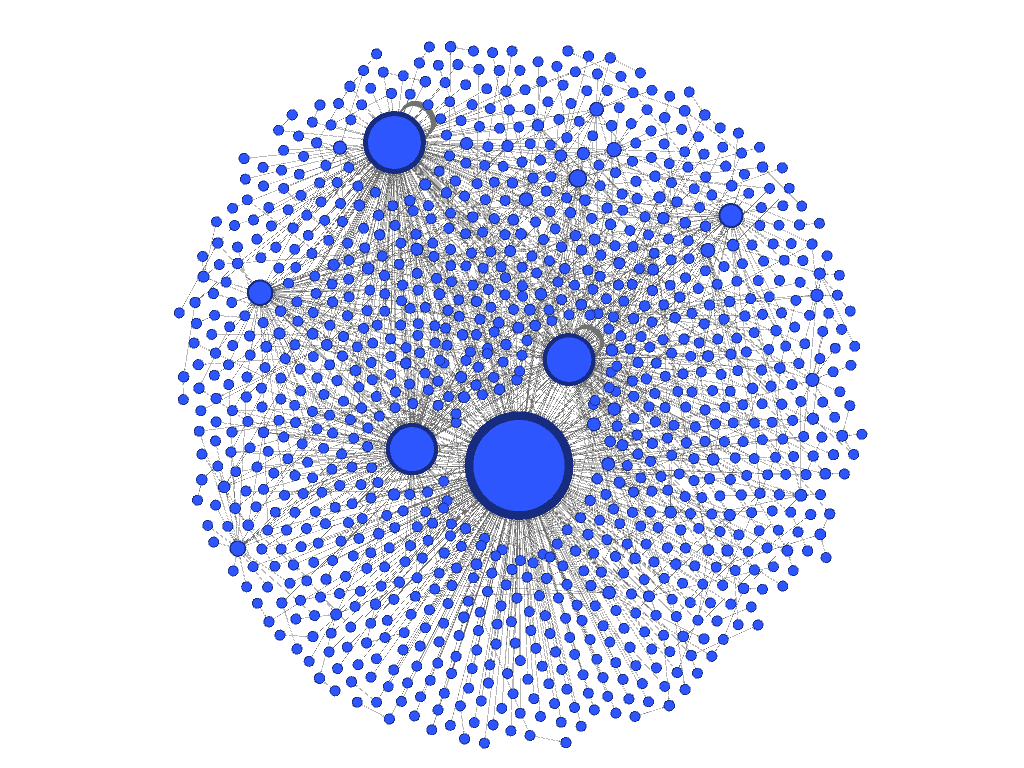
\includegraphics[scale=0.4]{images/init_1000_sf_1080_0.png}
\caption{Grafo rete scale-free, densità 0.1\%}
\label{fig:gsf}
\end{figure}
\subsubsection{Commento}
Da questi esperimenti possiamo trarre le seguenti considerazioni sugli obiettivi che ci eravamo posti:
\begin{description}
\item[Completamento della rete] Il nostro modello riesce a porre un limite alla crescita del numero di collegamenti; la rete, e quindi gli agenti, raggiungono una certa stabilità in prossimità di alcunoi valori di densità (circa tra il $7\%$ e l'$8\%$). Non avendo idea dell'entità della densità del grafo reale di Twitter, si può solo supporre che un certo valore di densità sia quello esatto; probabilmente un valore tra il $7\%$ e l'$8\%$ è ancora pittosto alto, c'è però margine per migliorarlo, andando a restringere acora di più i parametri descritti nella sezione \ref{sec:mod}.
\item[Invarianza di scala] Nella prima run, il nostro modello ha dimostrato che, data una configurazione di partenza del grafo a invarianza di scala, riesce a mantenere tale configurazione per tutto il periodo considerato. Nella altre quattro run, dove la rete è stata istanziata in modo randomico, in tre casi il nostro modello ha ``forzato" tutta la rete ad una configurazione assimilabile ad un paradigma scale free. Imputiamo la non riuscita dell'unico caso (rete randomica, densità 0.1\%) alla bassa densità di partenza, che, in un periodo di 1080 iterazioni, non è stato sufficiente a far entrare a pieno regime le meccaniche tipiche di una rete scale-free. C'è ancora margine di miglioramento su questo punto, ma confidiamo nella buona base di partenza offerta dalla nostra soluzione.
\end{description}
Altre considerazioni sono le seguenti:
\begin{description}
\item[Omofilia] La misura scelta per l'omofilia, ovvero l'\textit{assortatività per attributo}, non sembra aver fornito una risposta soddisfacente sul comportamento omofilo o meno degli agenti. In tutte le run l'indice si mostra parecchio irregolare, e comunque mai completamente positivo. Riteniamo che il problema non sia della metodologia usata per calcolare l'assortatività (piuttosto nota e utilizzata in letteratura), quanto nella rappresentazione dell'attributo di cui questa misura tiene conto: come già spiegato nella sezione \ref{sec:mod}, abbiamo ``condensato" un vettore di interessi in un solo attributo, corrispondente all'interesse con il valore maggiore all'interno del vettore; questo non coglie tutta l'informazione fornita da un vettore di valori, il quale viene usato dagli agenti per stabilire i collegamenti. L'informazione intercettata dall'indice è perciò incompleta. Un possibile miglioramento è senz'altro quello di trovare una misura alternativa, e più esaustiva.
\item[Ipotesi di small-world] Anche per l'ipotesi di small-world vale quanto affermato sulla densità reale di un social network come Twitter: è concesso solo supporre il valore reale del cammino minimo medio. In aggiunta, questa è una metrica che risente particolarmente della limitatezza intrinseca della simulazione: con solo 1000 agenti, il cammino minimo medio non può essere paragonato a quello di una rete che dispone di un numero di agenti maggiore di circa cinque ordini di grandezza, tanto più che non sempre in una simulazione si ha a che fare con un grafo connesso, come testimoniato nelle run. Ne concludiamo che l'ipotesi di small-world non possa essere verificata facilmente, se non con un lavoro di analisi su una rete reale. 
\end{description}
\subsection{Fase 2}
In questa fase, proponiamo la simulazione del seguente scenario: un utente ``hub" \textit{retwitta} un utente ``sconosciuto". L'obiettivo è studiare la variazione di in-degree dell'utente prescelto. La procedura è molto semplice, e si può riassumere così:
\begin{enumerate}
\item Ad una precisa iterazione, viene selezionato l'utente più popolare, ovvero con in-degree massimo, e quello meno popolare, con in-degree minimo.
\item Si crea un tweet ``fortunato" e lo si aggiunge alla lista di tweet generale
\item Si crea un retweet da parte dell'utente più popolare contenente il tweet fortunato e lo si aggiunge alla lista generale dei retweet.  
\end{enumerate}
Il tweet fortunato è caratterizzato dai seguenti parametri:
\begin{itemize}
\item Likability = 1
\item Dislikability = 0
\item Topic = scelto a caso dalla distribuzioni di topic del nodo ``hub"
\item Tag = nodo hub
\end{itemize}
Per le simulazioni abbiamo usato i due modelli migliori in base a quanto visto nella prima fase di esperimenti:
\begin{itemize}
\item Modello a invarianza di scala, densità $0.1\%$
\item Modello randomico, densità $1.0\%$
\end{itemize}
I parametri della simulazione sono gli stessi della fase 1.
L'iterazione prescelta per lo scatto di questo meccanismo è l'iterazione 400; l'abbiamo scelta in quanto lascia al modello 400 iterazioni per ``assestarsi", e 680 iterazioni per studiare il trend dell'in-degree.
\\ \\
L'obiettivo è, come già accennato, modellare il fatto realmente accaduto tra Termite e l'On. Gasparri nel 2012. Come in questo caso, ci aspettiamo che Termite (l'utente sconosciuto) abbia un picco di notorietà negli istanti immediatamente successivi all'evento (tweet fortunato), per poi stabilizzarsi se non addirittura descrescere. Da notare che il picco raggiunto da Termite era di circa 10.000 follower, quindi anche il massimo raggiunto durante le simulazioni dall'utente prescelto dovrebbe essere contenuto rispetto alle dimensioni della rete.
\subsubsection{Risultati}
Le figure \ref{fig:mat1}, \ref{fig:t1} e \ref{fig:g1} mostrano i trend per la simulazione della rete scale-free, mentre le figure \ref{fig:mat2}, \ref{fig:t2} e \ref{fig:g2} mostrano i trend per la rete randomica.
La figura \ref{fig:mat1} fornisce un quadro a grandi linee dell'andamento dell'in-degree della rete a invarianza di scala: durante il periodo di simulazione la maggior parte dei nodi rimane sotto la soglia dei 25 follower, mentre pochi altri spaziano tra questa soglia e i 300 collegamenti in entrata. Ogni nodo sembra manifestare un comportamento unico e non correlato a quello degli altri. In questa situazione abbiamo forzato l'evento di cui sopra. La figura \ref{fig:t1} mostra l'in-degree del nodo prescelto, mentre la figura \ref{fig:g1} mostra il trend del nodo ``hub" che l'ha retwittato. 
\begin{figure}[H]
\centering
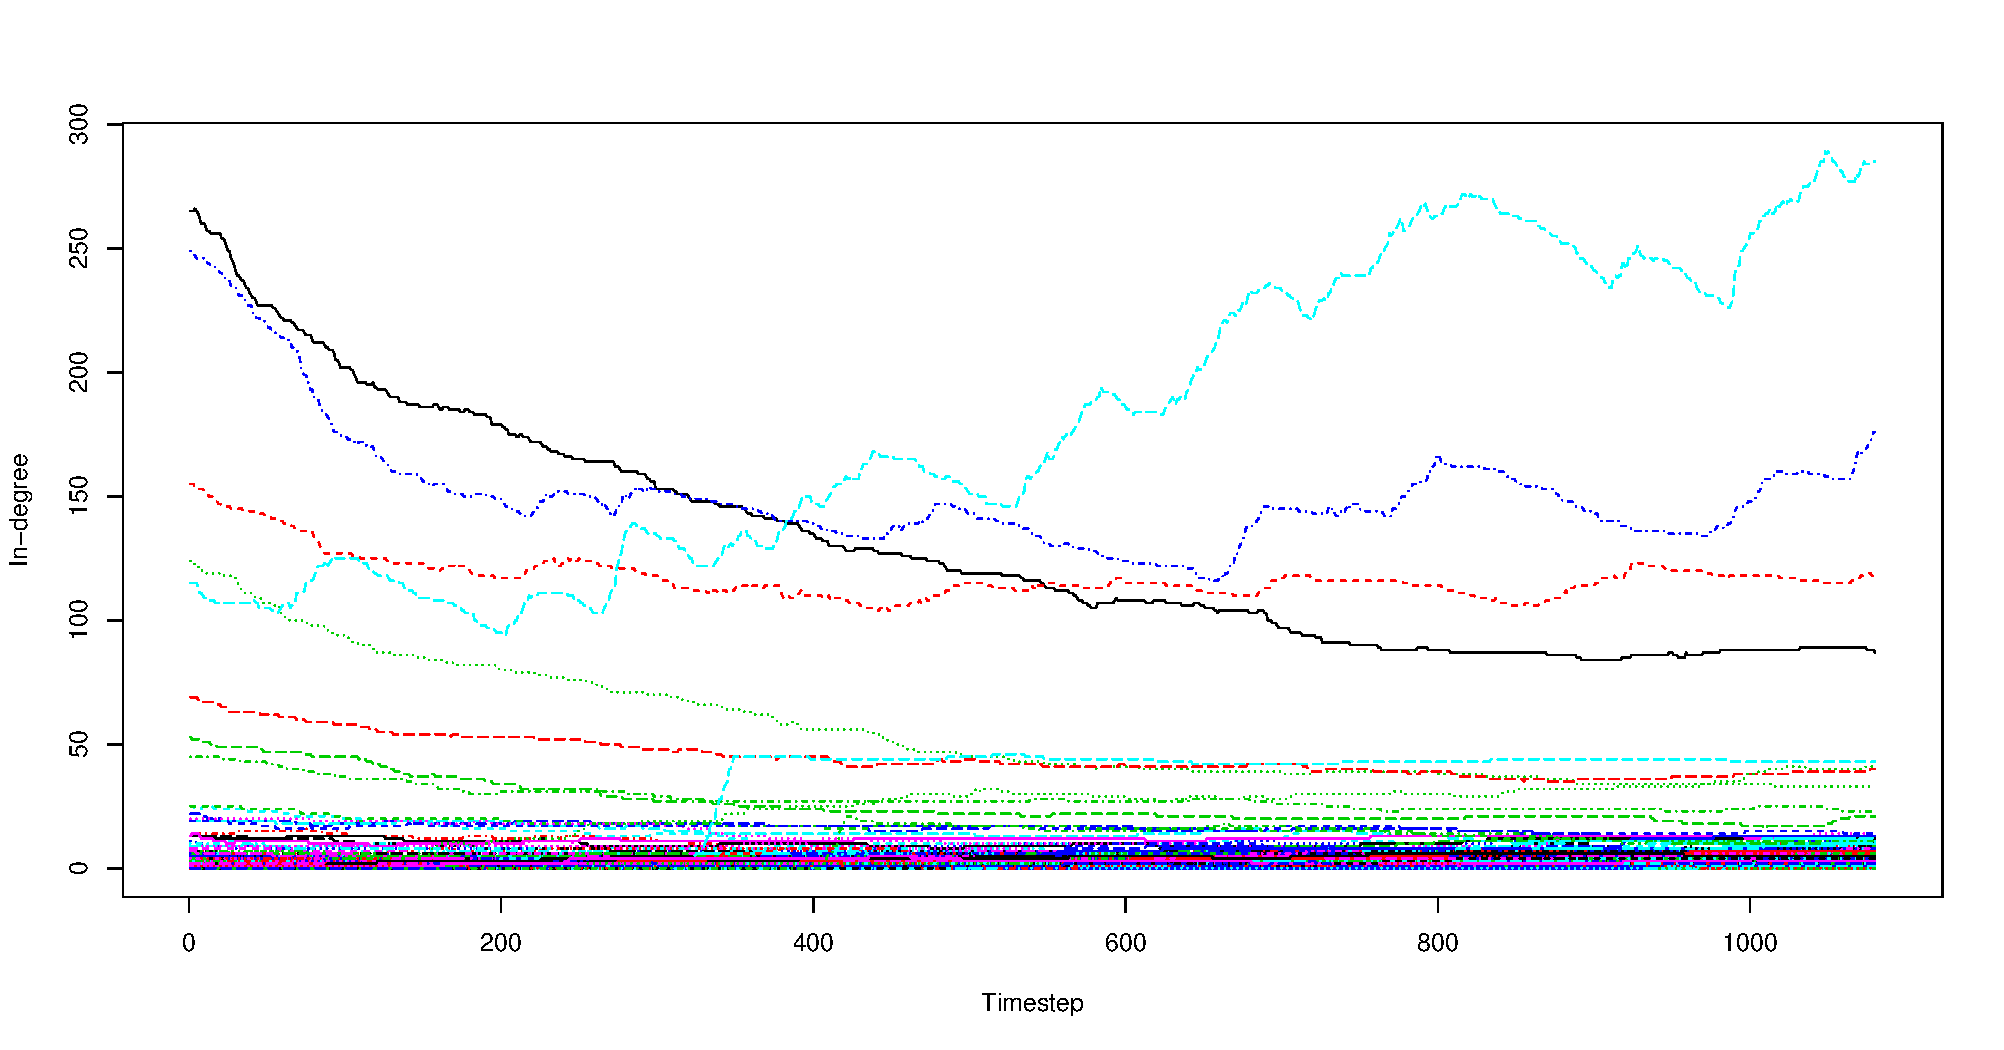
\includegraphics[scale=0.5]{images/totale_1000_sf_1080_1.pdf}
\caption{Andamento generale dell'in-degre dei nodi della rete scale-free}
\label{fig:mat1}
\end{figure}
Il numero di follower dell'utente prescelto si impenna subito dopo l'iterazione 400, fino a raggiungere il numero di 22 archi entranti. Le iterazioni successive sono caratterizzate da un generico calo dei follower, fino all'assestamento, intorno all'iterazione 950, su circa 15 seguaci. Prevedibilmente, il trend dell'utente popolare non risente del cambiamento, e continua la crescita fino alla terminazione. \\ \\
\begin{figure}[H]
\centering
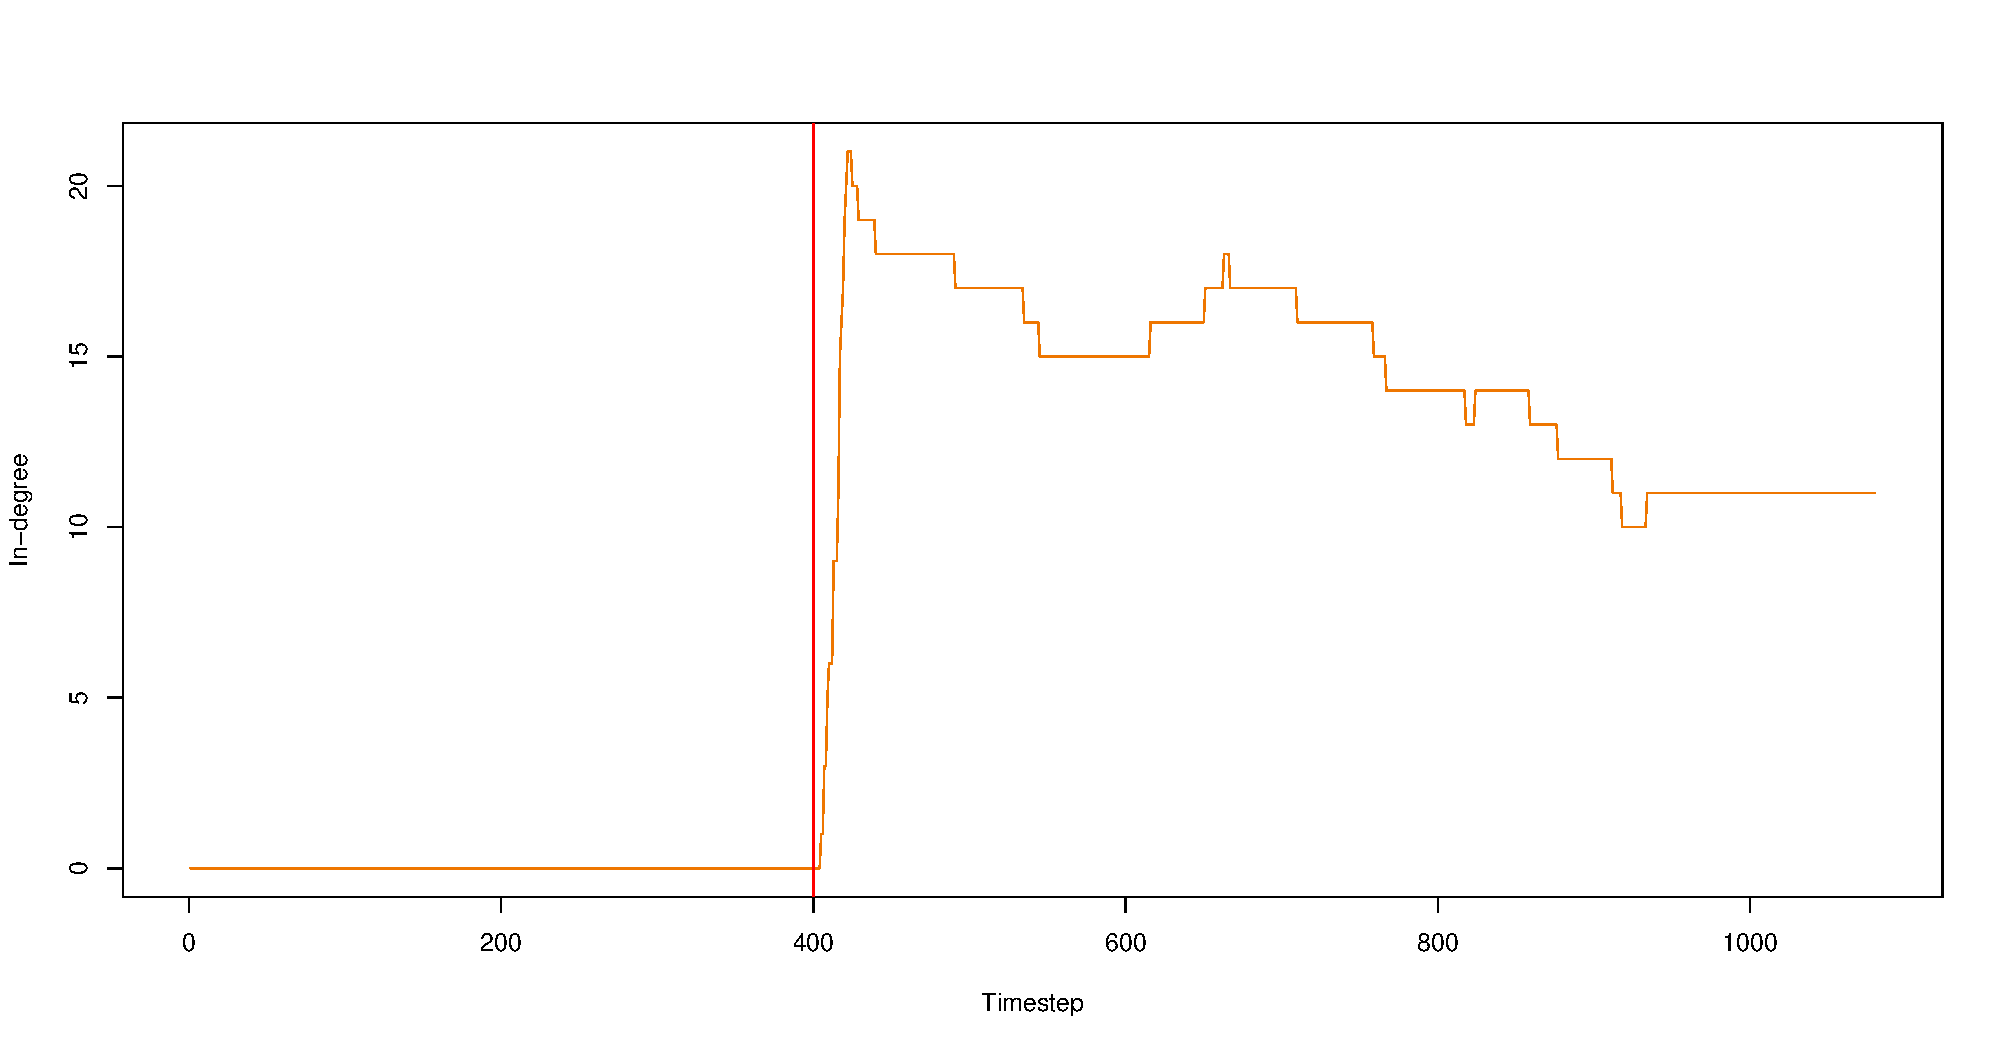
\includegraphics[scale=0.5]{images/prescelto_1000_sf_1080_1.pdf}
\caption{Andamento in-degree del nodo prescelto, nella rete scale-free}
\label{fig:t1}
\end{figure}
\begin{figure}[H]
\centering
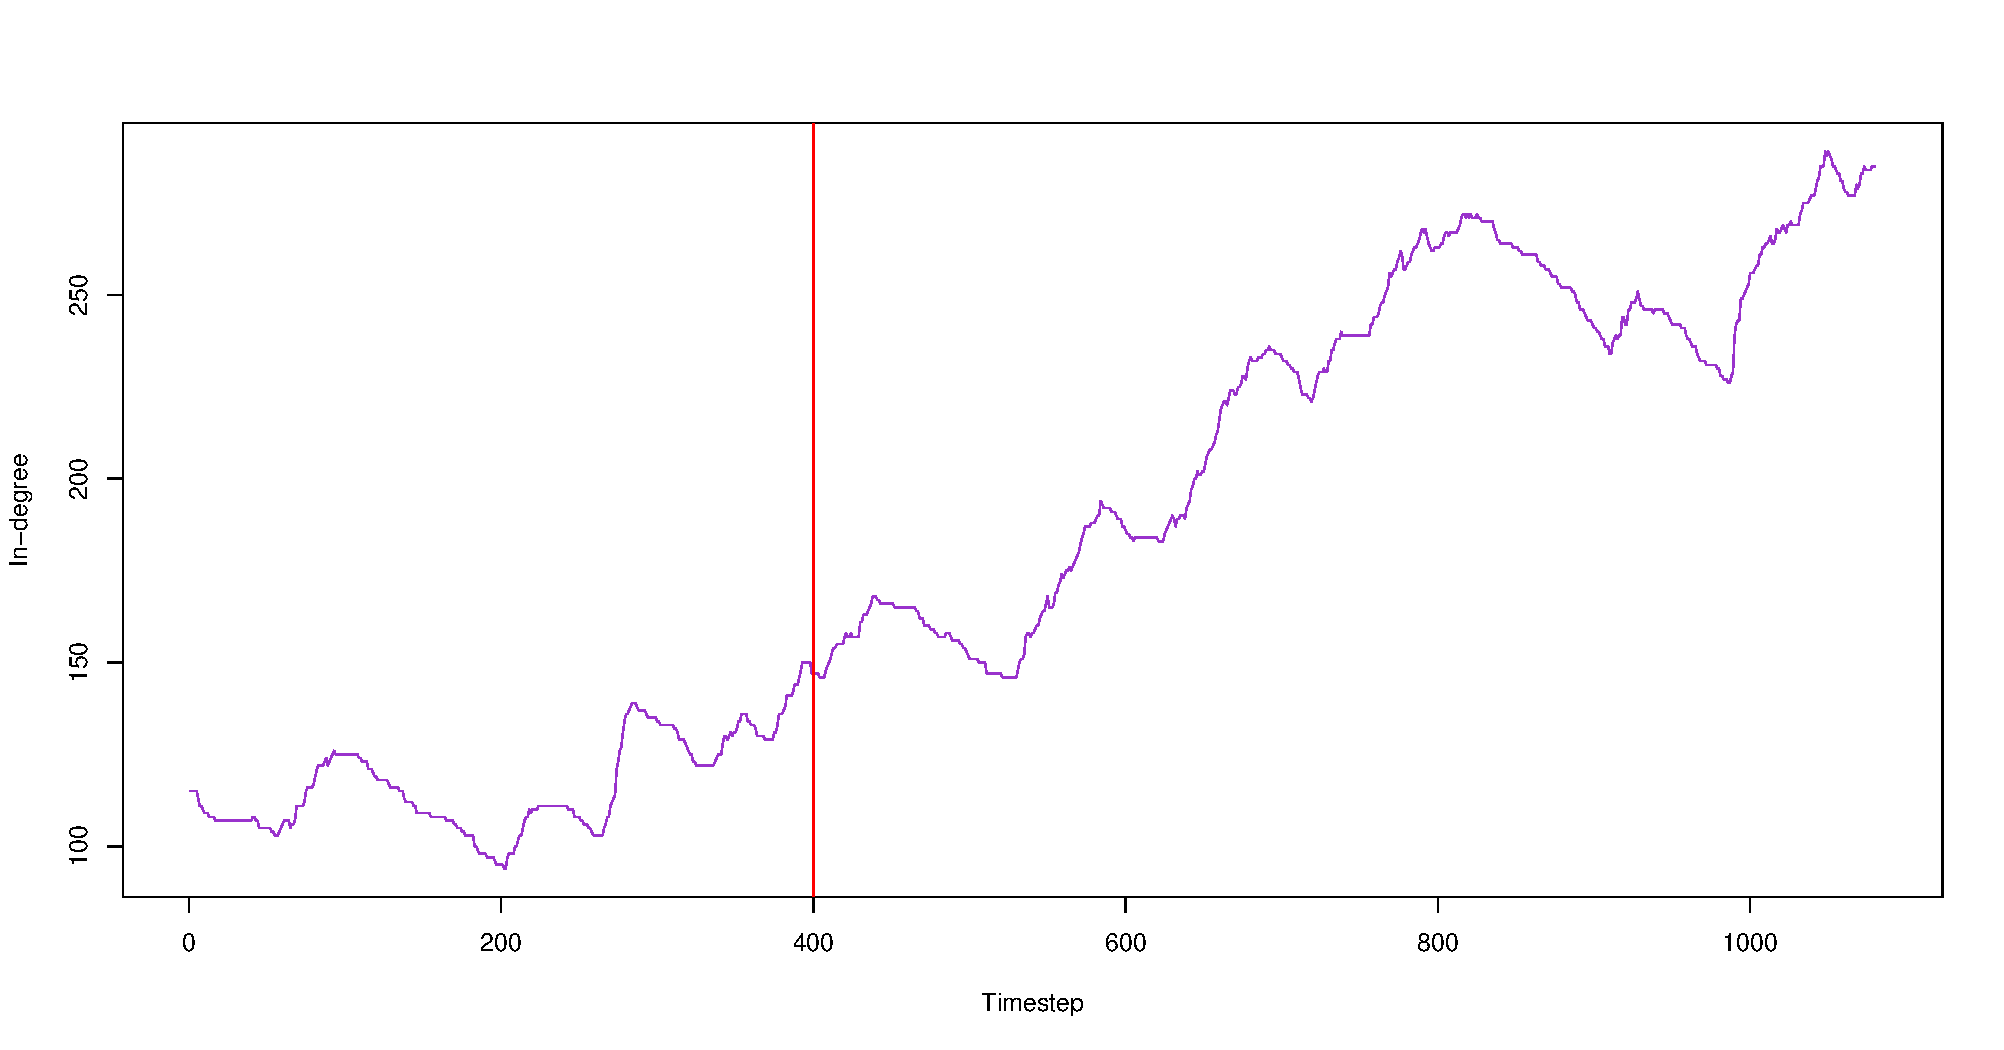
\includegraphics[scale=0.5]{images/gasparri_1000_sf_1080_1.pdf}
\caption{Andamento in-degree del nodo popolare, nella rete scale-free}
\label{fig:g1}
\end{figure}
Una situazione diversa si presenta nella simulazione con rete randomica. La figura \ref{fig:mat2} mostra un comportamento generale dei nodi piuttosto simile: sebbene la maggior parte rimanga confinata sotto i 100 follower (notare la differenza con la precedente simulazione, dovuta alla diversa densità), gli utenti popolari mostrano quasi tutti un comportamento crescente. Inoltre, questi nodi popolari sono molto più numerosi rispetto alla precedente simulazione. Questo fenomeno dovrebbe essere dovuto al processo descritto nella fase 1, secondo cui la rete randomica si ``trasforma" in una rete a invarianza di scala.
\begin{figure}[H]
\centering
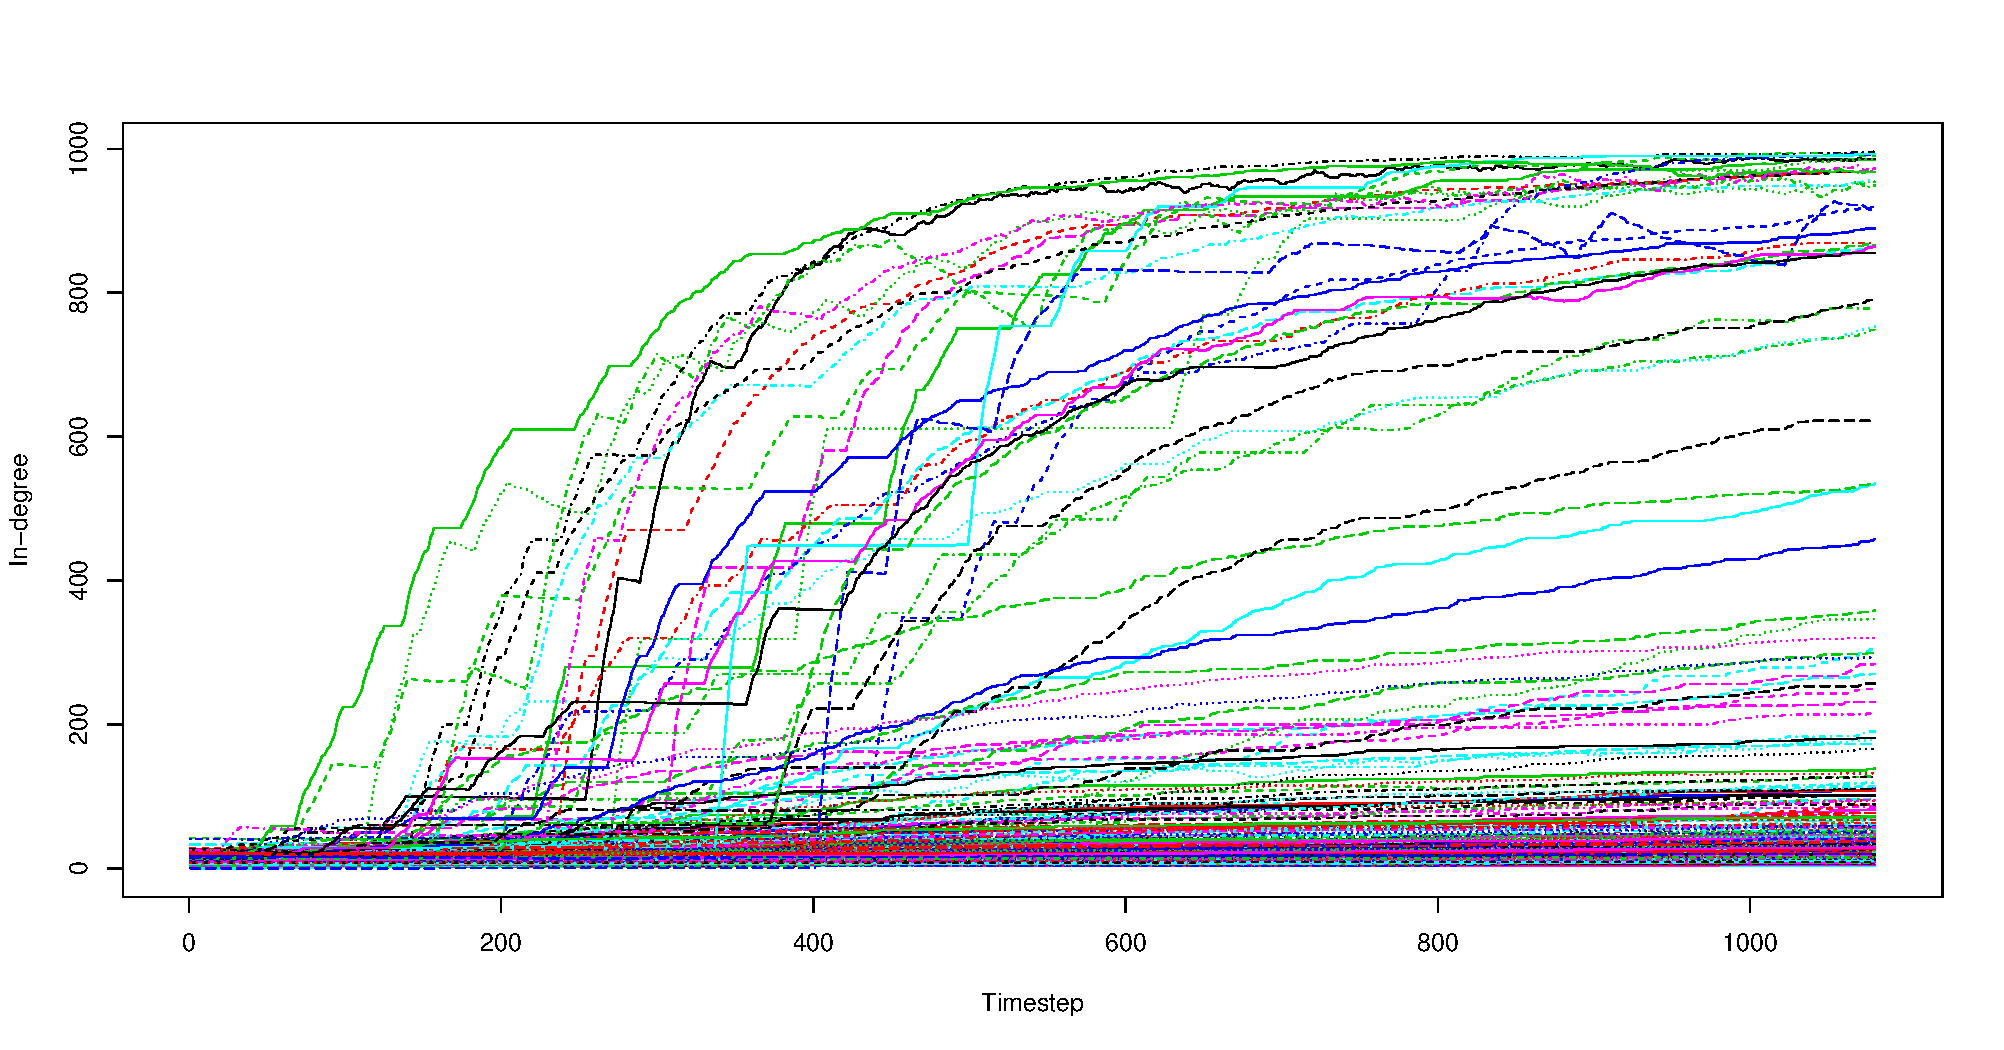
\includegraphics[scale=0.5]{images/totale_1000_rnd_1080_1_1.pdf}
\caption{Andamento generale dell'in-degre dei nodi della rete randomica}
\label{fig:mat2}
\end{figure}
\begin{figure}[H]
\centering
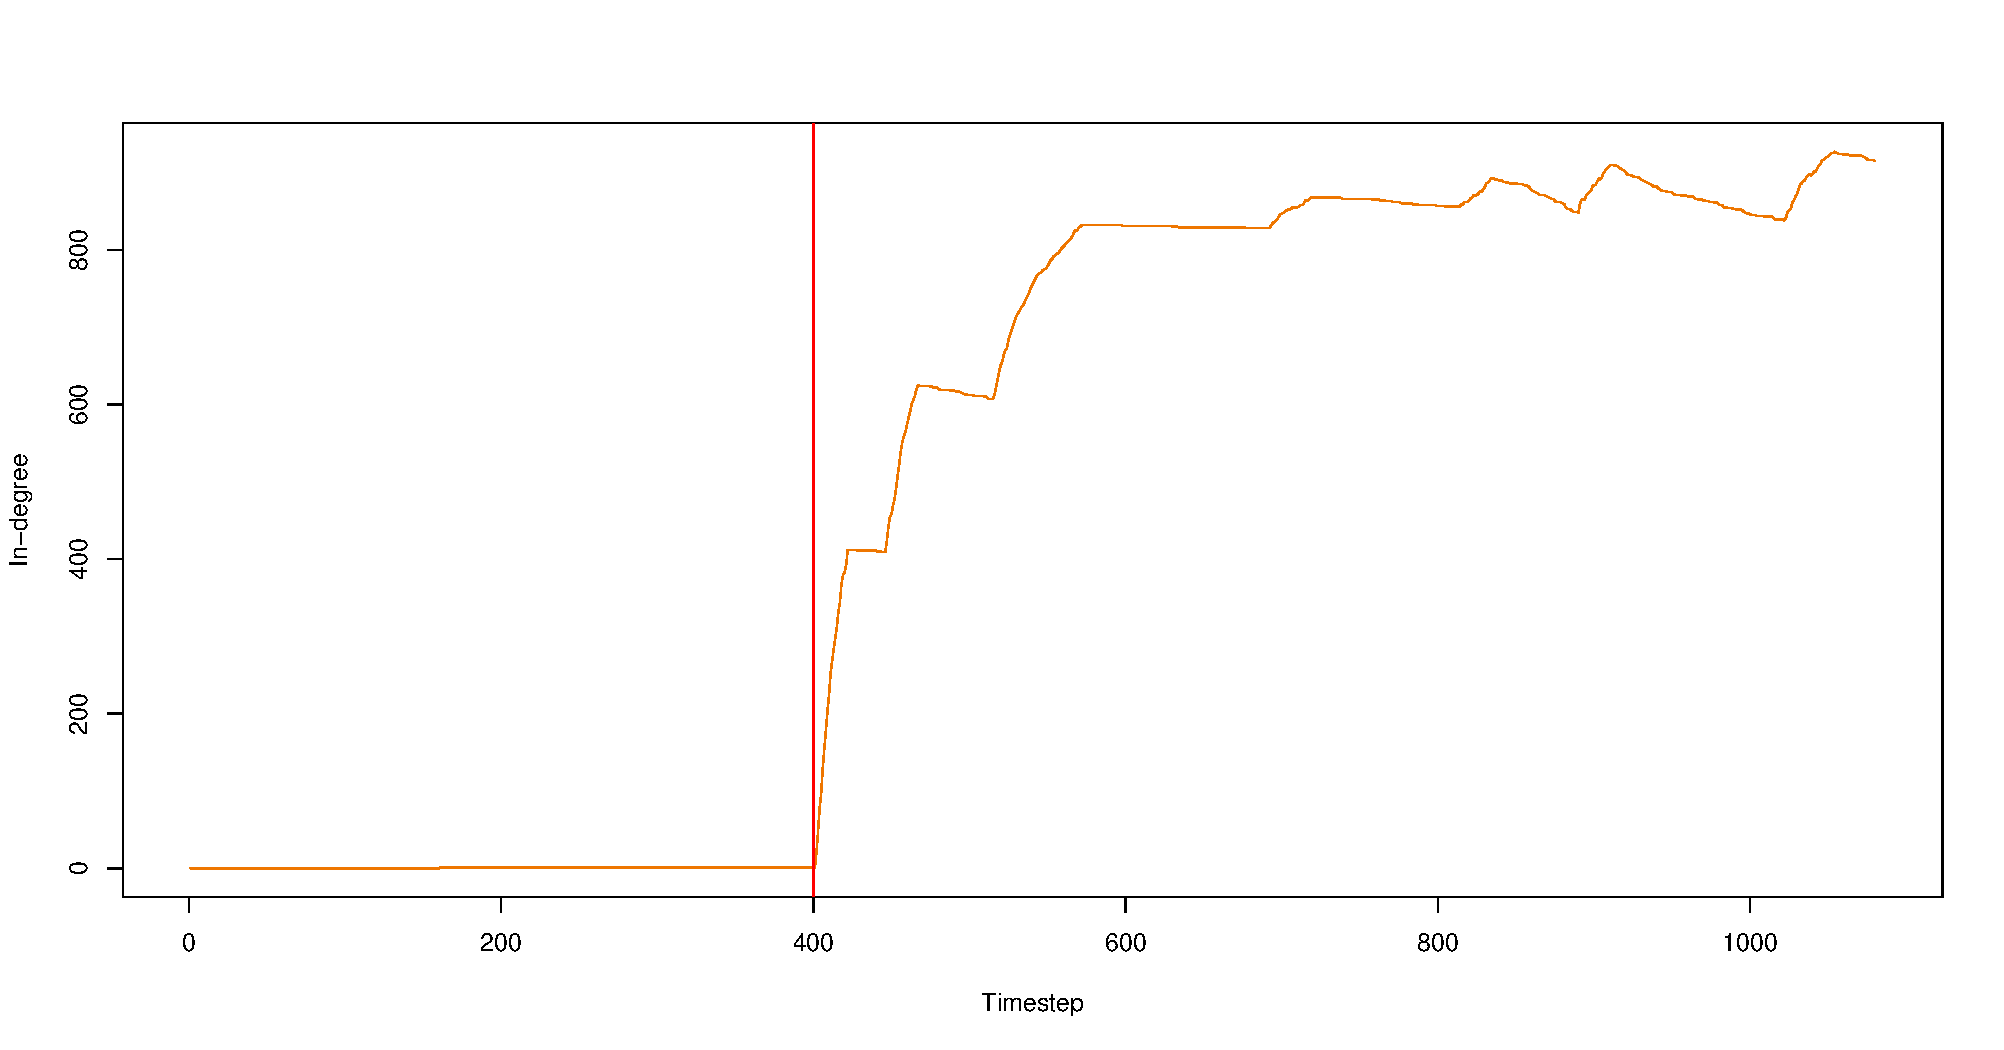
\includegraphics[scale=0.5]{images/prescelto_1000_rnd_1080_1_1.pdf}
\caption{Andamento in-degree del nodo prescelto, nella rete randomica}
\label{fig:t2}
\end{figure}
\begin{figure}[H]
\centering
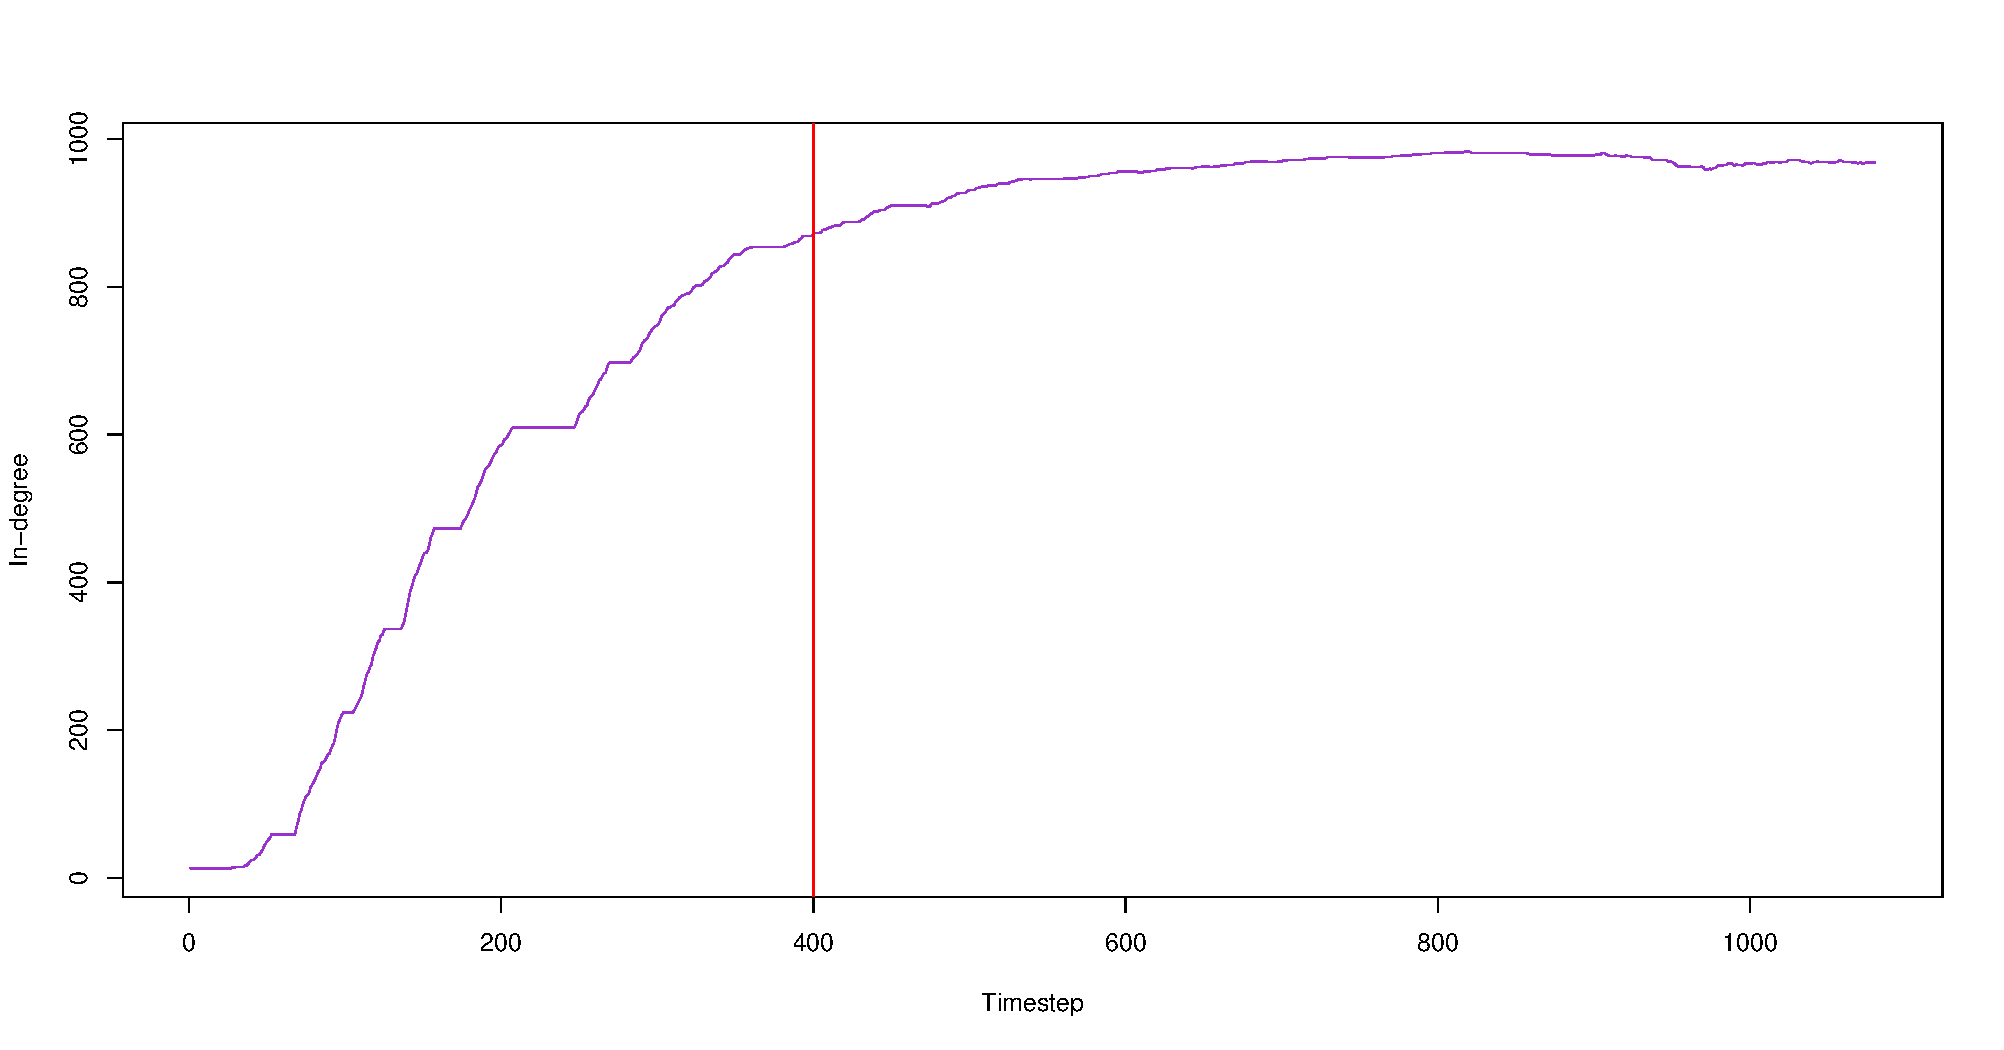
\includegraphics[scale=0.5]{images/gasparri_1000_rnd_1080_1_1.pdf}
\caption{Andamento in-degree del nodo popolare, nella rete randomica}
\label{fig:g2}
\end{figure}
In questo contesto è plausibile un andamento della curva dei follower del nodo prescelto come evidenziato dalla figura \ref{fig:t2} l'in-degree, da un valore inferiore a 20, si alza parecchio fino a superare il valore di 800 archi entranti, valore attorno al quale oscilla ma senza mai calare definitvamente. L'utente sconosciuto diventa nell'arco di pochissimo tempo un nodo ``hub" a tutti gli effetti. Questo è dovuto sicuramente alla maggiore densità iniziale, che accelera i cambiamenti all'interno della rete, e alla costruzione randomica iniziale, secondo quanto già evidenziato nella fase 1. Da notare anche la differenza di importanza dell'utente famoso tra la rete randomica e quella scale free: entrambi crescono fino alla fine delle iterazioni, ma mentre la crescita del nodo hub della rete scale-free è molto irregolare e il valore rimane sotto i 300 follower, la crescita della sua controparte in ambiente randomico (figura \ref{fig:g2}) è molto più regolare, fino al raggiungimento dei 1000 follower, il massimo possibile.
\subsubsection{Commento}
Dagli esperimenti condotti in questa fase è possibile trarre le seguenti conclusioni:
\begin{description}
\item[Rete scale-free] Il comportamento generale dei nodi sembra piuttosto ``naturale" e veritiero; in aggiunta, dopo il verificarsi dello scenario pianificato, la situazione che si viene a creare è molto simile a quella riscontrata nella realtà: l'utente sconosciuto cresce improvvisamente di popolarità, ma in modo contenuto rispetto alle dimensioni totali della rete. Dopo aver raggiunto il picco, i follower cominciano ad abbandonarlo, fino ad assestarsi su un valore intermedio tra i follower che aveva in precedenza ed il picco raggiunto. 
\item[Rete randomica] Nonostante il processo di ``metamorfosi" da rete randomica a rete scale-free che si verifica durante l'esecuzione del modello, la situazione che si viene a creare sembra non essere adatta alla simulazione di scenari. Il picco di popolarità ottenuto dal nodo prescelto è sproporzionato rispetto a quanto avvenuto nella realtà tra Termite e Gasparri.
Probabilmente gli agenti hanno bisogno di più tempo per stabilire trend di popolarità paragonabili a quelli riscontrati nella rete a invarianza di scala. Un fattore importante è sicuramente il limite alla crescita della densità, posto probabilmente troppo in alto ($7-8\%$): solo dopo il raggiungimento di questa soglia il comportamento dei nodi può differenziarsi.
\end{description}

\section{Conclusione e sviluppi futuri}
\label{sec:end}
Abbiamo qui esposto il nostro modello ABSoNeS e gli esperimenti condotti. In linea generale il modello può essere considerato come una buona base di partenza per la simulazione di Twitter, in quanto abbiamo verificato la prevenzione del completamento della rete e la proprietà ad invarianza di scala. In particolare, sia nella fase 1 che nella fase 2 delle prove è emerso come la configurazione iniziale della rete a invarianza di scala sia la migliore per conservarne le proprietà tipiche di una rete sociale e, successivamente, per simulare scenari. Resta il dubbio della densità iniziale, in quanto non è possibile stabilire la densità effettiva di Twitter: la rete a invarianza di scala limita la scelta della densità iniziale allo $0.1\%$, ma questo può essere aumentato manualmente con archi aggiunti in modo randomico, fino a raggiungere densità di partenza più elevata, seppur inquinando leggermente la power law. In questo modo si ridurrebbe inoltre il numero di nodi con grado $0$ presenti all'inizio delle run con bassa densità.  \\ \\
Le reti randomiche hanno il vantaggio principale nella scelta della densità iniziale, ma hanno bisogno di tempo per adattarsi alla soluzione modellistica da noi proposta. Infatti, sono servite a provare la limitatezza della crescita della densità, ma non hanno fornito l'ambiente necessario a simulare uno scenario.
\\ \\
Detto ciò, i possibili miglioramenti per ABSoNeS sono i seguenti:
\begin{description}
\item[Densità] Scongiurato il problema del completamento della rete, è emerso come il limite posto alla densità sia ancora troppo elevato. Un irrigidimento della probabilità di follow può ovviare a questo problema. In questo modo verrebbe garantita maggiormente la stabilità delle reti e un limite ai ``boom" di follower evidenziati soprattutto nelle reti random. 
\item[Dimensioni rete] Una simulazione di un sistema complesso difficilmente avrà le stesse dimensioni del sistema stesso: per ragioni implementative ne viene preso solo un pezzo o, come nela nostro caso, se ne crea una versione ridotta. \'E chiaro però che più la simulazione si avvicina come dimensioni al sistema reale, più può essere considerata attendibile; nel caso di social network, il numero di nodi dovrebbe essere quanto più alto possibile. Un possibile sviluppo futuro è dunque quello di aumentare il numero di nodi; un altra espansione in questi termini è quella di considerare la creazione e cancellazione di nodi. Nella realtà, infatti, nuovi utenti si aggiungono costantemente alla rete, e altri vengono eliminati. 
\item[Omofilia] Nella fase 1 degli esperimenti abbiamo constatato la limitatezza dell'assortatività per attributo come misura di omofilia. Purtroppo, networkx non ha implementazioni di questa metrica in grado di utilizzare attributi vettoriali. In \cite{mixing} viene fornita un'espansione della formula di assortatività in grado di misurare l'omofilia tenedo conto di attributi vettoriali: l'implementazione in Python di questa metrica sarebbe un primo passo per il miglioramento dell'analisi di omofilia. Inoltre, il vettore di interessi $PI$ può essere sostituito con una rappresentazione più ricca delle caratteristiche e degli interessi di un utente.
\item[Multithreading] L'aspetto implementativo sicuramente pi\`u interessante \`e la possibilit\`a di parallelizzare il modello, rendendo la simulazione molto pi\`u veloce permettendoci inoltre di aumentare la quantit\`a di nodi ed arco nel grafo iniziale e di permettere un aumento di grandezza dello stesso. Tuttavia non ci \`e stato possibile seguire questa strada implementativa per via delle restrizioni di Python. Abbiamo implementato il modello \textit{multi-threading} del linguaggio che per\`o risulta essere un modello che non parallelizza veramente il processo in quando nonostante pi\`u di un thread sia attivo sono tutti soggetti al controllo dell'interprete che \`e single core. La soluzione sarebbe quella di utilizzare il modello \textit{multi-processing} di Python, tuttavia questo richiede la gestione della concorrenza all'accesso e modifica delle strutture dati, e di conseguenza della memoria, relative alla simulazione. 
Una possibile strada da percorrere potrebbe quella di riscrivere l'intero modello in un linguaggio pi\`u a basso livello e pensato per una concorrenza sicura e stabile, come ad esempio \textbf{Rust}. Questa transizione porterebbe anche l'invalutabile vantaggio di accellerare notevolmente tutte le operazioni in quanto Rust \`e pensato per essere una alternativa pi\`u moderna e pi\`u memory-safe al C++, ed in quanto tale risulta avere velocit\`a paragonabili al C/C++ in quanto \`e compilato con lo stesso compilatore e utilizza le stesse librerie del C++. Si presuppone un aumento di prestazioni di circa il 130\% oltre ad una possibilit\`a di parallelizzare la parte pi\`u complessa e costosa in termini di tempo del modello, raggiungendo un aumento di velocit\`a inestimabile. 
Lo svantaggio pi\`u grande sarebbere quello di perdere la possibilt\`a di utilizzare la libreria NetworkX che oltre che essere estremamente ottimizzata contiene diversi parametri essenziali per la valutazione del risultato della simulazione.
\end{description}



\begin{thebibliography}{9}
\bibitem{facebook}
  Welch, Chris (2017). "Facebook crosses 2 billion monthly users". \textit{The Verge. Vox Media.} Retrieved June 27, 2017.
  
\bibitem{twitter}
  Bulman, May (2016). ``Donald Trump's 'celebrity-style' tweets helped him win US presidential election, says data scientist".
\textit{The Independent} Retrieved November 28, 2016.

\bibitem{youtube}
   Sorkin, Andrew Ross \& Peters, Jeremy, W. (2006). ``Google to Acquire YouTube for \$1.65 Billion". \textit{The New York Times.} Retrieved October 9, 2006.

\bibitem{linkedin}
   Greene, Jay (2016). ``Microsoft to Acquire LinkedIn for \$26.2 Billion". \textit{The Wall Street Journal.} Retrieved June 14, 2016.

\bibitem{gilbert}
  Hamill, L., \& Gilbert, N. (2010). Simulating large social networks in agent-based models: A social circle model. Emergence: Complexity and Organization, 12(4), 78.

\bibitem{barabasi}
  Barabási, A. L. (2016). Network science. Cambridge university press.
  
\bibitem{scalefree}
  Barabási, B. A. L., \& Bonabeau, E. (2003). Scale-free. Scientific American, 288(5), 50-59.
  
\bibitem{ferber}
  Ferber, J. (1999). Multi-agent systems: an introduction to distributed artificial intelligence (Vol. 1). Reading: Addison-Wesley.
ISO 690	

\bibitem{link}
  Liben-Nowell, D., \& Kleinberg, J. (2007). The link-prediction problem for social networks. journal of the Association for Information Science and Technology, 58(7), 1019-1031.
  
\bibitem{katz}
  Katz, L. (1953). A new status index derived from sociometric analysis. Psychometrika, 18(1), 39-43.

\bibitem{google}
  Brin, S., \& Page, L. (2012). Reprint of: The anatomy of a large-scale hypertextual web search engine. Computer networks, 56(18), 3825-3833.

\bibitem{homo}
  McPherson, M., Smith-Lovin, L., \& Cook, J. M. (2001). Birds of a feather: Homophily in social networks. Annual review of sociology, 27(1), 415-444.
  
\bibitem{group}
  Currarini, S., Jackson, M. O., \& Pin, P. (2009). An economic model of friendship: Homophily, minorities, and segregation. Econometrica, 77(4), 1003-1045.
  
\bibitem{red}
  Zeng, R., Sheng, Q. Z., Yao, L., Xu, T., \& Xie, D. (2013, January). A practical simulation method for social networks. In Proceedings of the First Australasian Web Conference-Volume 144 (pp. 27-34). Australian Computer Society, Inc..
  
\bibitem{det}
  Singer, H. M., Singer, I., \& Herrmann, H. J. (2009). Agent-based model for friendship in social networks. Physical Review E, 80(2), 026113.

\bibitem{ir}
  Manning, C. D., Raghavan, P., \& Schütze, H. (2008). Introduction to information retrieval. Cambridge University Press.
  
\bibitem{cormen}
  Cormen, T. H., Leiserson, C. E., Rivest, R. L., \& Stein, C. (2001). Introduction to algorithms second edition. McGraw-Hill.
  
\bibitem{newman}
  Newman, M. (2010). Networks: an introduction. Oxford university press.
  
\bibitem{nx}
  Hagberg, A., Swart, P., \& S Chult, D. (2008). Exploring network structure, dynamics, and function using NetworkX (No. LA-UR-08-05495; LA-UR-08-5495). Los Alamos National Laboratory (LANL).
ISO 690	

\bibitem{assor}
  Foster, J. G., Foster, D. V., Grassberger, P., \& Paczuski, M. (2010). Edge direction and the structure of networks. Proceedings of the National Academy of Sciences, 107(24), 10815-10820.
  
\bibitem{mixing}
  Newman, M. E. (2003). Mixing patterns in networks. Physical Review E, 67(2), 026126.
  
\bibitem{termite}
  Spotti, V (2012). \# EPICFAILGasparri, i signori Nessuno e gli eroi del giorno ai tempi di Twitter. www.techeconomy.it
  
\bibitem{sfnx}
  Bollobás, B., Borgs, C., Chayes, J., \& Riordan, O. (2003, January). Directed scale-free graphs. In Proceedings of the fourteenth annual ACM-SIAM symposium on Discrete algorithms (pp. 132-139). Society for Industrial and Applied Mathematics.
\end{thebibliography}
\end{document}